\documentclass[twoside]{book}

% Packages required by doxygen
\usepackage{fixltx2e}
\usepackage{calc}
\usepackage{doxygen}
\usepackage[export]{adjustbox} % also loads graphicx
\usepackage{graphicx}
\usepackage[utf8]{inputenc}
\usepackage{makeidx}
\usepackage{multicol}
\usepackage{multirow}
\PassOptionsToPackage{warn}{textcomp}
\usepackage{textcomp}
\usepackage[nointegrals]{wasysym}
\usepackage[table]{xcolor}

% Font selection
\usepackage[T1]{fontenc}
\usepackage[scaled=.90]{helvet}
\usepackage{courier}
\usepackage{amssymb}
\usepackage{sectsty}
\renewcommand{\familydefault}{\sfdefault}
\allsectionsfont{%
  \fontseries{bc}\selectfont%
  \color{darkgray}%
}
\renewcommand{\DoxyLabelFont}{%
  \fontseries{bc}\selectfont%
  \color{darkgray}%
}
\newcommand{\+}{\discretionary{\mbox{\scriptsize$\hookleftarrow$}}{}{}}

% Page & text layout
\usepackage{geometry}
\geometry{%
  a4paper,%
  top=2.5cm,%
  bottom=2.5cm,%
  left=2.5cm,%
  right=2.5cm%
}
\tolerance=750
\hfuzz=15pt
\hbadness=750
\setlength{\emergencystretch}{15pt}
\setlength{\parindent}{0cm}
\setlength{\parskip}{3ex plus 2ex minus 2ex}
\makeatletter
\renewcommand{\paragraph}{%
  \@startsection{paragraph}{4}{0ex}{-1.0ex}{1.0ex}{%
    \normalfont\normalsize\bfseries\SS@parafont%
  }%
}
\renewcommand{\subparagraph}{%
  \@startsection{subparagraph}{5}{0ex}{-1.0ex}{1.0ex}{%
    \normalfont\normalsize\bfseries\SS@subparafont%
  }%
}
\makeatother

% Headers & footers
\usepackage{fancyhdr}
\pagestyle{fancyplain}
\fancyhead[LE]{\fancyplain{}{\bfseries\thepage}}
\fancyhead[CE]{\fancyplain{}{}}
\fancyhead[RE]{\fancyplain{}{\bfseries\leftmark}}
\fancyhead[LO]{\fancyplain{}{\bfseries\rightmark}}
\fancyhead[CO]{\fancyplain{}{}}
\fancyhead[RO]{\fancyplain{}{\bfseries\thepage}}
\fancyfoot[LE]{\fancyplain{}{}}
\fancyfoot[CE]{\fancyplain{}{}}
\fancyfoot[RE]{\fancyplain{}{\bfseries\scriptsize Generated on Mon May 2 2016 23\+:02\+:55 for Holum by Doxygen }}
\fancyfoot[LO]{\fancyplain{}{\bfseries\scriptsize Generated on Mon May 2 2016 23\+:02\+:55 for Holum by Doxygen }}
\fancyfoot[CO]{\fancyplain{}{}}
\fancyfoot[RO]{\fancyplain{}{}}
\renewcommand{\footrulewidth}{0.4pt}
\renewcommand{\chaptermark}[1]{%
  \markboth{#1}{}%
}
\renewcommand{\sectionmark}[1]{%
  \markright{\thesection\ #1}%
}

% Indices & bibliography
\usepackage{natbib}
\usepackage[titles]{tocloft}
\setcounter{tocdepth}{3}
\setcounter{secnumdepth}{5}
\makeindex

% Hyperlinks (required, but should be loaded last)
\usepackage{ifpdf}
\ifpdf
  \usepackage[pdftex,pagebackref=true]{hyperref}
\else
  \usepackage[ps2pdf,pagebackref=true]{hyperref}
\fi
\hypersetup{%
  colorlinks=true,%
  linkcolor=blue,%
  citecolor=blue,%
  unicode%
}

% Custom commands
\newcommand{\clearemptydoublepage}{%
  \newpage{\pagestyle{empty}\cleardoublepage}%
}

\usepackage{caption}
\captionsetup{labelsep=space,justification=centering,font={bf},singlelinecheck=off,skip=4pt,position=top}

%===== C O N T E N T S =====

\begin{document}

% Titlepage & ToC
\hypersetup{pageanchor=false,
             bookmarksnumbered=true,
             pdfencoding=unicode
            }
\pagenumbering{roman}
\begin{titlepage}
\vspace*{7cm}
\begin{center}%
{\Large Holum \\[1ex]\large 1.\+0 }\\
\vspace*{1cm}
{\large Generated by Doxygen 1.8.11}\\
\vspace*{0.5cm}
{\small Mon May 2 2016 23:02:55}\\
\end{center}
\end{titlepage}
\clearemptydoublepage
\tableofcontents
\clearemptydoublepage
\pagenumbering{arabic}
\hypersetup{pageanchor=true}

%--- Begin generated contents ---
\chapter{Holum}
\label{index}\hypertarget{index}{}\subsubsection*{Obiettivi del progetto}

Holum è un progetto che focalizza i suoi obiettivi su usabilità, intuitività ed efficienza. È progettato per utenti di ogni età e possiede una varietà di caratteristiche che possono essere utilizzate per soddisfare una vasta gamma di interessi ed esigenze. Si rivolge sia a utenti non specializzati o solo in parte avvertiti delle attività di programmazione informatica, sia a vari tipi di utenti specializzati, senza precludere nessuna tipologia.

L’obiettivo primario è quindi quello di sviluppare un software in grado di offrire varie funzionalità, tra cui la possibilità di {\bfseries riproduzione multimediale} di filmati, sia pre-\/caricati appositamente dagli sviluppatori, che tramite la scelta dell’utente. Inoltre, l’utilizzatore potrà caricare e visualizzare {\bfseries modelli tridimensionali}, con la possibilità di ingrandire, ruotare e traslare il modello in questione, tramite alcuni sistemi di interazione. Un’altra funzionalità riguarda la creazione di un insieme di {\bfseries videogiochi}, realizzati con lo scopo di intrattenimento e svago dell’utente.

Ogni funzionalità del programma dovrà essere personalizzabile tramite la selezione di impostazioni adeguate alle preferenze e alle esigenze dell’utente. L’insieme di questi sottoprogrammi verrà poi raccolto e reso accessibile in un apposito {\bfseries menù}.

L’interazione con il software dovrà avvenire tramite alcuni dispositivi in grado di raccogliere informazioni sulle scelte dell’utente, per poi tradurle in un linguaggio comprensibile dal calcolatore. Queste informazioni verrano quindi utilizzate per navigare all’interno del menù e del programma in generale.

Il software avrà anche il principale compito di suddividere l’immagine da visualizzare in 4 “parti” uguali, a due a due simmetriche e speculari. Il software dovrà poi essere accompagnato da un’appropriato {\bfseries sistema piramidale}, sostenuto da una struttura di supporto. Questa struttura dovrà sorreggere un monitor, il quale si occuperà di visualizzare l’immagine prodotta dal software. Infine, la superficie riflettente della piramide, assieme alla suddivisione dell’immagine da visualizzare, dovrà creare il desiderato {\bfseries effetto di tridimensionalità e profondità della proiezione nello spazio}.

\subsubsection*{Specifiche tecniche}

L’effetto utilizzato per la riproduzione delle immagini è conosciuto come {\bfseries “\+Pepper’s Ghost”}, ovvero il “\+Fantasma di Pepper”\+: una tecnica illusoria utilizzata in teatro e in vari trucchi magici che consiste nell’utilizzo di una o più lastre di vetro, posizionate ad un angolo di 45˚ tra lo spettatore e la scena, unite a una particolare illuminazione, per dare l’illusione della rappresentazione nello spazio delle immagini proiettate. Il contenuto che verrà proiettato sarà riprodotto da un software appositamente programmato, utilizzando il linguaggio C++ e le librerie {\bfseries S\+F\+ML, sfe\+Movie, Open\+GL, assimp} e altre.

L\textquotesingle{}utente può quindi, come accennato sopra, interagire con il programma in diversi modi\+:
\begin{DoxyItemize}
\item {\bfseries Utility Android}, sviluppata in Java, attualmente strutturata per la sola navigazione all’interno del software su PC, tramite connessione bluetooth;
\item {\bfseries Myo Armband} (\href{https://www.myo.com}{\tt https\+://www.\+myo.\+com}), un braccialetto “smart” che tramite la la lettura dei movimenti muscolari permette il controllo wireless del software, utilizzando appositi gesti e movimenti. Per realizzare il collegamento con il programma in C++ abbiamo utilizzato la libreria myo, personalizzandone alcune funzioni per adattarla alle nostre esigenze;
\item {\bfseries Leap Motion} (\href{https://www.leapmotion.com}{\tt https\+://www.\+leapmotion.\+com}), un dispositivo in grado di rilevare accuratamente il movimento di dita e mani dell’utente nello spazio sovrastante al dispositivo stesso, permettendo l’interazione con il software in C++ tramite l’apposito S\+DK offerto da Leap Motion.
\end{DoxyItemize}

Il programma offrirà la riproduzione di una serie di mini-\/giochi, pensati opportunamente per sfruttare al meglio le potenzialità dei dispositivi in questione. Tramite questi controller è quindi possibile spostarsi all\textquotesingle{}interno dei menù e del programma, il quale offre varie categorie di intrattenimento.

La schermata iniziale, successiva allo splash screen di benvenuto, presenta il menù, suddiviso nelle seguenti sezioni\+:
\begin{DoxyItemize}
\item {\bfseries \hyperlink{classVideo}{Video}}\+: Archivio di filmati pensati appositamente per la rappresentazione nella piramide. I video pre-\/caricati sono caratterizzati da uno sfondo nero e da una riproduzione tridimensionale dei caratteri raffigurati, per garantirne l’ottimale visualizzazione e favorire l’illusione della raffigurazione di un simil-\/ologramma;
\item {\bfseries Games}\+: Sezione dedicata ai giochi, sia inerenti al Leap Motion che non. I giochi presenti potranno essere selezionati dall’utente tramite un menù, simile a quello principale;
\item {\bfseries 3D}\+: Sezione dedicata al caricamento e alla rappresentazione di un archivio di modelli 3D in formato O\+BJ, tramite le funzionalità offerte da Open\+GL. L’utente potrà interagire con il modello tramite un controller a sua scelta;
\item {\bfseries \hyperlink{classSettings}{Settings}}\+: Gestione delle preferenze utente riguardanti l’interfaccia grafica, audio e dei controller.
\end{DoxyItemize}

\subsubsection*{Ruoli e responsabilità}


\begin{DoxyItemize}
\item {\bfseries Eusebio Apopei} (Costruttore, Programmatore)\+: Ha il ruolo di realizzare, sia in fase prototipale che definitiva, la struttura piramidale e quella reggente. Si occuperà anche di svolgere il compito di programmatore di parte del software, tra cui l\textquotesingle{}utility per sistema operativo Android.
\item {\bfseries Davide Cosentino} (Grafico, Programmatore)\+: Ha il ruolo di realizzare l\textquotesingle{}interfaccia grafica del programma e di sviluppare una parte del software, tra cui l\textquotesingle{}utility per sistema operativo Android.
\item {\bfseries Alessio Falai} (Project \hyperlink{classManager}{Manager}, Sviluppatore Software)\+: Ha il ruolo di coordinare tutte le attività del progetto e di supervisionare il corretto svolgimento dei lavori. Si occuperà anche di svolgere il compito di analista e programmatore di parte del software e di interfacciare i dispositivi di H\+ID (Human Interface Device) con il software generale.
\item {\bfseries Lorenzo Pratesi} (Sviluppatore Software)\+: Svolge il principale compito di analista e programmatore software del progetto. Si occuperà anche di interfacciare i dispositivi di H\+ID (Human Interface Device) con il software generale.
\item {\bfseries Vittorio Sodini} (Grafico, Programmatore)\+: Ha il ruolo di realizzare l’interfaccia grafica del programma e di sviluppare una parte del software, tra cui l\textquotesingle{}utility per sistema operativo Android. 
\end{DoxyItemize}
\chapter{Namespace Index}
\section{Namespace List}
Here is a list of all namespaces with brief descriptions\+:\begin{DoxyCompactList}
\item\contentsline{section}{\hyperlink{namespacesh}{sh} \\*It is used to distinguish Holum shaders from S\+F\+ML ones }{\pageref{namespacesh}}{}
\end{DoxyCompactList}

\chapter{Hierarchical Index}
\section{Class Hierarchy}
This inheritance list is sorted roughly, but not completely, alphabetically\+:\begin{DoxyCompactList}
\item \contentsline{section}{Bluetooth}{\pageref{classBluetooth}}{}
\item Device\+Listener\begin{DoxyCompactList}
\item \contentsline{section}{Myo\+Connector}{\pageref{classMyoConnector}}{}
\end{DoxyCompactList}
\item \contentsline{section}{File}{\pageref{classFile}}{}
\item Listener\begin{DoxyCompactList}
\item \contentsline{section}{Leap\+Listener}{\pageref{classLeapListener}}{}
\end{DoxyCompactList}
\item \contentsline{section}{Manager}{\pageref{classManager}}{}
\item \contentsline{section}{Menu}{\pageref{classMenu}}{}
\item \contentsline{section}{Mesh}{\pageref{classMesh}}{}
\item \contentsline{section}{Mesh\+:\+:texture}{\pageref{structMesh_1_1texture}}{}
\item \contentsline{section}{Mesh\+:\+:vertex}{\pageref{structMesh_1_1vertex}}{}
\item \contentsline{section}{Model}{\pageref{classModel}}{}
\item \contentsline{section}{Settings}{\pageref{classSettings}}{}
\item \contentsline{section}{sh\+:\+:Shader}{\pageref{classsh_1_1Shader}}{}
\item \contentsline{section}{ThreeD}{\pageref{classThreeD}}{}
\item \contentsline{section}{Video}{\pageref{classVideo}}{}
\end{DoxyCompactList}

\chapter{Data Structure Index}
\section{Data Structures}
Here are the data structures with brief descriptions\+:\begin{DoxyCompactList}
\item\contentsline{section}{\hyperlink{classBluetooth}{Bluetooth} \\*Wireless communication between this software and the Android application }{\pageref{classBluetooth}}{}
\item\contentsline{section}{\hyperlink{classFile}{File} \\*Describes resources relative to the \hyperlink{classVideo}{Video} and \hyperlink{classThreeD}{ThreeD} sections }{\pageref{classFile}}{}
\item\contentsline{section}{\hyperlink{classLeapListener}{Leap\+Listener} \\*Data transfers between this software and the Leap Motion device }{\pageref{classLeapListener}}{}
\item\contentsline{section}{\hyperlink{classManager}{Manager} }{\pageref{classManager}}{}
\item\contentsline{section}{\hyperlink{classMenu}{Menu} }{\pageref{classMenu}}{}
\item\contentsline{section}{\hyperlink{classMesh}{Mesh} \\*Defines each single drawable entity, in a format that Open\+GL uses to render the objects }{\pageref{classMesh}}{}
\item\contentsline{section}{\hyperlink{structMesh_1_1texture}{Mesh\+::texture} \\*It is used to organize the material data, in the form of textures }{\pageref{structMesh_1_1texture}}{}
\item\contentsline{section}{\hyperlink{structMesh_1_1vertex}{Mesh\+::vertex} \\*It is a set of vectors which contains a position vector, a normal vector and a texture coordinate vector }{\pageref{structMesh_1_1vertex}}{}
\item\contentsline{section}{\hyperlink{classModel}{Model} }{\pageref{classModel}}{}
\item\contentsline{section}{\hyperlink{classMyoConnector}{Myo\+Connector} \\*A \hyperlink{classMyoConnector}{Myo\+Connector} object receives and processes events about a Myo }{\pageref{classMyoConnector}}{}
\item\contentsline{section}{\hyperlink{classSettings}{Settings} }{\pageref{classSettings}}{}
\item\contentsline{section}{\hyperlink{classsh_1_1Shader}{sh\+::\+Shader} \\*Describes the little programs, which rest on the G\+PU, used in the rendering operation next to an Open\+GL drawing command execution }{\pageref{classsh_1_1Shader}}{}
\item\contentsline{section}{\hyperlink{classThreeD}{ThreeD} }{\pageref{classThreeD}}{}
\item\contentsline{section}{\hyperlink{classVideo}{Video} \\*Describes the G\+UI and the functions relative to the video playback section }{\pageref{classVideo}}{}
\end{DoxyCompactList}

\chapter{File Index}
\section{File List}
Here is a list of all files with brief descriptions\+:\begin{DoxyCompactList}
\item\contentsline{section}{\hyperlink{Bluetooth_8h}{Bluetooth.\+h} }{\pageref{Bluetooth_8h}}{}
\item\contentsline{section}{\hyperlink{File_8h}{File.\+h} }{\pageref{File_8h}}{}
\item\contentsline{section}{\hyperlink{Global_8h}{Global.\+h} }{\pageref{Global_8h}}{}
\item\contentsline{section}{\hyperlink{LeapListener_8h}{Leap\+Listener.\+h} }{\pageref{LeapListener_8h}}{}
\item\contentsline{section}{\hyperlink{Libraries_8h}{Libraries.\+h} }{\pageref{Libraries_8h}}{}
\item\contentsline{section}{\hyperlink{Manager_8h}{Manager.\+h} }{\pageref{Manager_8h}}{}
\item\contentsline{section}{\hyperlink{Menu_8h}{Menu.\+h} }{\pageref{Menu_8h}}{}
\item\contentsline{section}{\hyperlink{Mesh_8h}{Mesh.\+h} }{\pageref{Mesh_8h}}{}
\item\contentsline{section}{\hyperlink{Model_8h}{Model.\+h} }{\pageref{Model_8h}}{}
\item\contentsline{section}{\hyperlink{MyoConnector_8h}{Myo\+Connector.\+h} }{\pageref{MyoConnector_8h}}{}
\item\contentsline{section}{\hyperlink{Settings_8h}{Settings.\+h} }{\pageref{Settings_8h}}{}
\item\contentsline{section}{\hyperlink{Shader_8h}{Shader.\+h} }{\pageref{Shader_8h}}{}
\item\contentsline{section}{\hyperlink{ThreeD_8h}{Three\+D.\+h} }{\pageref{ThreeD_8h}}{}
\item\contentsline{section}{\hyperlink{Video_8h}{Video.\+h} }{\pageref{Video_8h}}{}
\end{DoxyCompactList}

\chapter{Namespace Documentation}
\hypertarget{namespacesh}{}\section{sh Namespace Reference}
\label{namespacesh}\index{sh@{sh}}


It is used to distinguish Holum shaders from S\+F\+ML ones.  


\subsection*{Data Structures}
\begin{DoxyCompactItemize}
\item 
class \hyperlink{classsh_1_1Shader}{Shader}
\begin{DoxyCompactList}\small\item\em The \hyperlink{classsh_1_1Shader}{Shader} class describes the little programs, which rest on the G\+PU, used in the rendering operation next to an Open\+GL drawing command execution. \end{DoxyCompactList}\end{DoxyCompactItemize}

\chapter{Data Structure Documentation}
\hypertarget{classBluetooth}{}\section{Bluetooth Class Reference}
\label{classBluetooth}\index{Bluetooth@{Bluetooth}}


The \hyperlink{classBluetooth}{Bluetooth} class provides wireless communication between this software and the Android application.  




{\ttfamily \#include $<$Bluetooth.\+h$>$}

\subsection*{Public Member Functions}
\begin{DoxyCompactItemize}
\item 
\hyperlink{classBluetooth_adff22f9e5f2bd81b1fc5b8eeba71f68b}{Bluetooth} ()
\item 
\hyperlink{classBluetooth_a89e37d06353e375c0c05d02caca60e7a}{Bluetooth} (const \hyperlink{classBluetooth}{Bluetooth} \&b)
\item 
bool \hyperlink{classBluetooth_a1d1d79331f7ac176240617f864c90986}{accept\+Socket} ()
\item 
bool \hyperlink{classBluetooth_a9b72d26b9ca3954c61b07aa31a29b87a}{bind\+Socket} ()
\item 
bool \hyperlink{classBluetooth_a7a14c1d4892ab911f24fe241c0f9d8bd}{check\+Message} ()
\item 
void \hyperlink{classBluetooth_ad827d394aff7e1b67b552e77c939fe97}{close\+Socket} ()
\item 
int \hyperlink{classBluetooth_a06b93309bc14bf3c8c1522a859b46a93}{get\+Direction} ()
\item 
bool \hyperlink{classBluetooth_afb4dda9fe9df7c2ebf02efdafe17bc5f}{init} ()
\item 
bool \hyperlink{classBluetooth_a5355c79812948221e6f0c9c47b191b8a}{is\+Available} ()
\item 
void \hyperlink{classBluetooth_aa6cd9fe9e9d0472579d53c79d0a3e644}{is\+Available} (bool \hyperlink{classBluetooth_a6a16541ed58b634caff713ca4209e975}{available})
\item 
bool \hyperlink{classBluetooth_aae394d2379c39a67d9efbca886da9e25}{listen\+Socket} ()
\item 
void \hyperlink{classBluetooth_ae13d797ede1bb492eded4285142a7f3c}{manage\+Bluetooth} ()
\item 
int \hyperlink{classBluetooth_a9bcc560b34605070e72b2b285b1d4f16}{read\+Message} ()
\item 
bool \hyperlink{classBluetooth_a1b1b147c12429192e8ef7e543e6e4d67}{register\+Service} ()
\item 
void \hyperlink{classBluetooth_acee37e1c96d3b1f39ace4d58c43190bf}{start\+Communication} ()
\end{DoxyCompactItemize}
\subsection*{Private Attributes}
\begin{DoxyCompactItemize}
\item 
atomic\+\_\+bool \hyperlink{classBluetooth_a6a16541ed58b634caff713ca4209e975}{available}
\item 
Clock \hyperlink{classBluetooth_ae66d43274ae46b6895b0132258e5cf1e}{clock}
\item 
Clock \hyperlink{classBluetooth_a2494be6c40b4071bf13c6a018d635a7d}{clock2}
\item 
atomic\+\_\+int \hyperlink{classBluetooth_ad0f51dfcfb452953467ee9eec3801725}{direction}
\item 
bool \hyperlink{classBluetooth_acca56b0089cf38cd2f2a4d0d7d330360}{exit}
\item 
Time \hyperlink{classBluetooth_a9bb41383c492dc0919dfa6d026bc718d}{time}
\end{DoxyCompactItemize}


\subsection{Constructor \& Destructor Documentation}
\index{Bluetooth@{Bluetooth}!Bluetooth@{Bluetooth}}
\index{Bluetooth@{Bluetooth}!Bluetooth@{Bluetooth}}
\subsubsection[{\texorpdfstring{Bluetooth()}{Bluetooth()}}]{\setlength{\rightskip}{0pt plus 5cm}Bluetooth\+::\+Bluetooth (
\begin{DoxyParamCaption}
{}
\end{DoxyParamCaption}
)}\hypertarget{classBluetooth_adff22f9e5f2bd81b1fc5b8eeba71f68b}{}\label{classBluetooth_adff22f9e5f2bd81b1fc5b8eeba71f68b}
\index{Bluetooth@{Bluetooth}!Bluetooth@{Bluetooth}}
\index{Bluetooth@{Bluetooth}!Bluetooth@{Bluetooth}}
\subsubsection[{\texorpdfstring{Bluetooth(const Bluetooth \&b)}{Bluetooth(const Bluetooth &b)}}]{\setlength{\rightskip}{0pt plus 5cm}Bluetooth\+::\+Bluetooth (
\begin{DoxyParamCaption}
\item[{const {\bf Bluetooth} \&}]{b}
\end{DoxyParamCaption}
)}\hypertarget{classBluetooth_a89e37d06353e375c0c05d02caca60e7a}{}\label{classBluetooth_a89e37d06353e375c0c05d02caca60e7a}


\subsection{Member Function Documentation}
\index{Bluetooth@{Bluetooth}!accept\+Socket@{accept\+Socket}}
\index{accept\+Socket@{accept\+Socket}!Bluetooth@{Bluetooth}}
\subsubsection[{\texorpdfstring{accept\+Socket()}{acceptSocket()}}]{\setlength{\rightskip}{0pt plus 5cm}bool Bluetooth\+::accept\+Socket (
\begin{DoxyParamCaption}
{}
\end{DoxyParamCaption}
)}\hypertarget{classBluetooth_a1d1d79331f7ac176240617f864c90986}{}\label{classBluetooth_a1d1d79331f7ac176240617f864c90986}
\index{Bluetooth@{Bluetooth}!bind\+Socket@{bind\+Socket}}
\index{bind\+Socket@{bind\+Socket}!Bluetooth@{Bluetooth}}
\subsubsection[{\texorpdfstring{bind\+Socket()}{bindSocket()}}]{\setlength{\rightskip}{0pt plus 5cm}bool Bluetooth\+::bind\+Socket (
\begin{DoxyParamCaption}
{}
\end{DoxyParamCaption}
)}\hypertarget{classBluetooth_a9b72d26b9ca3954c61b07aa31a29b87a}{}\label{classBluetooth_a9b72d26b9ca3954c61b07aa31a29b87a}
\index{Bluetooth@{Bluetooth}!check\+Message@{check\+Message}}
\index{check\+Message@{check\+Message}!Bluetooth@{Bluetooth}}
\subsubsection[{\texorpdfstring{check\+Message()}{checkMessage()}}]{\setlength{\rightskip}{0pt plus 5cm}bool Bluetooth\+::check\+Message (
\begin{DoxyParamCaption}
{}
\end{DoxyParamCaption}
)}\hypertarget{classBluetooth_a7a14c1d4892ab911f24fe241c0f9d8bd}{}\label{classBluetooth_a7a14c1d4892ab911f24fe241c0f9d8bd}
\index{Bluetooth@{Bluetooth}!close\+Socket@{close\+Socket}}
\index{close\+Socket@{close\+Socket}!Bluetooth@{Bluetooth}}
\subsubsection[{\texorpdfstring{close\+Socket()}{closeSocket()}}]{\setlength{\rightskip}{0pt plus 5cm}void Bluetooth\+::close\+Socket (
\begin{DoxyParamCaption}
{}
\end{DoxyParamCaption}
)}\hypertarget{classBluetooth_ad827d394aff7e1b67b552e77c939fe97}{}\label{classBluetooth_ad827d394aff7e1b67b552e77c939fe97}
\index{Bluetooth@{Bluetooth}!get\+Direction@{get\+Direction}}
\index{get\+Direction@{get\+Direction}!Bluetooth@{Bluetooth}}
\subsubsection[{\texorpdfstring{get\+Direction()}{getDirection()}}]{\setlength{\rightskip}{0pt plus 5cm}int Bluetooth\+::get\+Direction (
\begin{DoxyParamCaption}
{}
\end{DoxyParamCaption}
)}\hypertarget{classBluetooth_a06b93309bc14bf3c8c1522a859b46a93}{}\label{classBluetooth_a06b93309bc14bf3c8c1522a859b46a93}
\index{Bluetooth@{Bluetooth}!init@{init}}
\index{init@{init}!Bluetooth@{Bluetooth}}
\subsubsection[{\texorpdfstring{init()}{init()}}]{\setlength{\rightskip}{0pt plus 5cm}bool Bluetooth\+::init (
\begin{DoxyParamCaption}
{}
\end{DoxyParamCaption}
)}\hypertarget{classBluetooth_afb4dda9fe9df7c2ebf02efdafe17bc5f}{}\label{classBluetooth_afb4dda9fe9df7c2ebf02efdafe17bc5f}
\index{Bluetooth@{Bluetooth}!is\+Available@{is\+Available}}
\index{is\+Available@{is\+Available}!Bluetooth@{Bluetooth}}
\subsubsection[{\texorpdfstring{is\+Available()}{isAvailable()}}]{\setlength{\rightskip}{0pt plus 5cm}bool Bluetooth\+::is\+Available (
\begin{DoxyParamCaption}
{}
\end{DoxyParamCaption}
)}\hypertarget{classBluetooth_a5355c79812948221e6f0c9c47b191b8a}{}\label{classBluetooth_a5355c79812948221e6f0c9c47b191b8a}
\index{Bluetooth@{Bluetooth}!is\+Available@{is\+Available}}
\index{is\+Available@{is\+Available}!Bluetooth@{Bluetooth}}
\subsubsection[{\texorpdfstring{is\+Available(bool available)}{isAvailable(bool available)}}]{\setlength{\rightskip}{0pt plus 5cm}void Bluetooth\+::is\+Available (
\begin{DoxyParamCaption}
\item[{bool}]{available}
\end{DoxyParamCaption}
)}\hypertarget{classBluetooth_aa6cd9fe9e9d0472579d53c79d0a3e644}{}\label{classBluetooth_aa6cd9fe9e9d0472579d53c79d0a3e644}
\index{Bluetooth@{Bluetooth}!listen\+Socket@{listen\+Socket}}
\index{listen\+Socket@{listen\+Socket}!Bluetooth@{Bluetooth}}
\subsubsection[{\texorpdfstring{listen\+Socket()}{listenSocket()}}]{\setlength{\rightskip}{0pt plus 5cm}bool Bluetooth\+::listen\+Socket (
\begin{DoxyParamCaption}
{}
\end{DoxyParamCaption}
)}\hypertarget{classBluetooth_aae394d2379c39a67d9efbca886da9e25}{}\label{classBluetooth_aae394d2379c39a67d9efbca886da9e25}
\index{Bluetooth@{Bluetooth}!manage\+Bluetooth@{manage\+Bluetooth}}
\index{manage\+Bluetooth@{manage\+Bluetooth}!Bluetooth@{Bluetooth}}
\subsubsection[{\texorpdfstring{manage\+Bluetooth()}{manageBluetooth()}}]{\setlength{\rightskip}{0pt plus 5cm}void Bluetooth\+::manage\+Bluetooth (
\begin{DoxyParamCaption}
{}
\end{DoxyParamCaption}
)}\hypertarget{classBluetooth_ae13d797ede1bb492eded4285142a7f3c}{}\label{classBluetooth_ae13d797ede1bb492eded4285142a7f3c}
\index{Bluetooth@{Bluetooth}!read\+Message@{read\+Message}}
\index{read\+Message@{read\+Message}!Bluetooth@{Bluetooth}}
\subsubsection[{\texorpdfstring{read\+Message()}{readMessage()}}]{\setlength{\rightskip}{0pt plus 5cm}int Bluetooth\+::read\+Message (
\begin{DoxyParamCaption}
{}
\end{DoxyParamCaption}
)}\hypertarget{classBluetooth_a9bcc560b34605070e72b2b285b1d4f16}{}\label{classBluetooth_a9bcc560b34605070e72b2b285b1d4f16}
\index{Bluetooth@{Bluetooth}!register\+Service@{register\+Service}}
\index{register\+Service@{register\+Service}!Bluetooth@{Bluetooth}}
\subsubsection[{\texorpdfstring{register\+Service()}{registerService()}}]{\setlength{\rightskip}{0pt plus 5cm}bool Bluetooth\+::register\+Service (
\begin{DoxyParamCaption}
{}
\end{DoxyParamCaption}
)}\hypertarget{classBluetooth_a1b1b147c12429192e8ef7e543e6e4d67}{}\label{classBluetooth_a1b1b147c12429192e8ef7e543e6e4d67}
\index{Bluetooth@{Bluetooth}!start\+Communication@{start\+Communication}}
\index{start\+Communication@{start\+Communication}!Bluetooth@{Bluetooth}}
\subsubsection[{\texorpdfstring{start\+Communication()}{startCommunication()}}]{\setlength{\rightskip}{0pt plus 5cm}void Bluetooth\+::start\+Communication (
\begin{DoxyParamCaption}
{}
\end{DoxyParamCaption}
)}\hypertarget{classBluetooth_acee37e1c96d3b1f39ace4d58c43190bf}{}\label{classBluetooth_acee37e1c96d3b1f39ace4d58c43190bf}


\subsection{Field Documentation}
\index{Bluetooth@{Bluetooth}!available@{available}}
\index{available@{available}!Bluetooth@{Bluetooth}}
\subsubsection[{\texorpdfstring{available}{available}}]{\setlength{\rightskip}{0pt plus 5cm}atomic\+\_\+bool Bluetooth\+::available\hspace{0.3cm}{\ttfamily [private]}}\hypertarget{classBluetooth_a6a16541ed58b634caff713ca4209e975}{}\label{classBluetooth_a6a16541ed58b634caff713ca4209e975}
\index{Bluetooth@{Bluetooth}!clock@{clock}}
\index{clock@{clock}!Bluetooth@{Bluetooth}}
\subsubsection[{\texorpdfstring{clock}{clock}}]{\setlength{\rightskip}{0pt plus 5cm}Clock Bluetooth\+::clock\hspace{0.3cm}{\ttfamily [private]}}\hypertarget{classBluetooth_ae66d43274ae46b6895b0132258e5cf1e}{}\label{classBluetooth_ae66d43274ae46b6895b0132258e5cf1e}
\index{Bluetooth@{Bluetooth}!clock2@{clock2}}
\index{clock2@{clock2}!Bluetooth@{Bluetooth}}
\subsubsection[{\texorpdfstring{clock2}{clock2}}]{\setlength{\rightskip}{0pt plus 5cm}Clock Bluetooth\+::clock2\hspace{0.3cm}{\ttfamily [private]}}\hypertarget{classBluetooth_a2494be6c40b4071bf13c6a018d635a7d}{}\label{classBluetooth_a2494be6c40b4071bf13c6a018d635a7d}
\index{Bluetooth@{Bluetooth}!direction@{direction}}
\index{direction@{direction}!Bluetooth@{Bluetooth}}
\subsubsection[{\texorpdfstring{direction}{direction}}]{\setlength{\rightskip}{0pt plus 5cm}atomic\+\_\+int Bluetooth\+::direction\hspace{0.3cm}{\ttfamily [private]}}\hypertarget{classBluetooth_ad0f51dfcfb452953467ee9eec3801725}{}\label{classBluetooth_ad0f51dfcfb452953467ee9eec3801725}
\index{Bluetooth@{Bluetooth}!exit@{exit}}
\index{exit@{exit}!Bluetooth@{Bluetooth}}
\subsubsection[{\texorpdfstring{exit}{exit}}]{\setlength{\rightskip}{0pt plus 5cm}bool Bluetooth\+::exit\hspace{0.3cm}{\ttfamily [private]}}\hypertarget{classBluetooth_acca56b0089cf38cd2f2a4d0d7d330360}{}\label{classBluetooth_acca56b0089cf38cd2f2a4d0d7d330360}
\index{Bluetooth@{Bluetooth}!time@{time}}
\index{time@{time}!Bluetooth@{Bluetooth}}
\subsubsection[{\texorpdfstring{time}{time}}]{\setlength{\rightskip}{0pt plus 5cm}Time Bluetooth\+::time\hspace{0.3cm}{\ttfamily [private]}}\hypertarget{classBluetooth_a9bb41383c492dc0919dfa6d026bc718d}{}\label{classBluetooth_a9bb41383c492dc0919dfa6d026bc718d}


The documentation for this class was generated from the following file\+:\begin{DoxyCompactItemize}
\item 
\hyperlink{Bluetooth_8h}{Bluetooth.\+h}\end{DoxyCompactItemize}

\hypertarget{classFile}{}\section{File Class Reference}
\label{classFile}\index{File@{File}}


The \hyperlink{classFile}{File} class describes resources relative to the \hyperlink{classVideo}{Video} and \hyperlink{classThreeD}{ThreeD} sections.  




{\ttfamily \#include $<$File.\+h$>$}

\subsection*{Public Member Functions}
\begin{DoxyCompactItemize}
\item 
\hyperlink{classFile_ae039af5807fc385f41b60644725d15d0}{File} ()
\item 
\hyperlink{classFile_a1ede4d44b5010bf25d3550af017b3f38}{File} (string \hyperlink{classFile_afd963fd6ba55fa762f7d3ab962e97e6c}{path}, string \hyperlink{classFile_a302a98ac2a5820e288e9be26d5947bc4}{title})
\item 
string \hyperlink{classFile_afba45549e5ffb4741dc1da7e242f16d8}{get\+Path} ()
\item 
Rectangle\+Shape $\ast$ \hyperlink{classFile_a29e127bbe05e9d28b803502ed7284339}{get\+Thumbnail} ()
\item 
string \hyperlink{classFile_a3ef33194903dba59d7ca995cbcee97f1}{get\+Thumbnail\+Path} ()
\item 
Vector2f \hyperlink{classFile_a6291b69f260763ee5b7b866759d84f86}{get\+Thumbnail\+Position} ()
\item 
Vector2f \hyperlink{classFile_a391872e43babdf3f7102e344580f6bee}{get\+Thumbnail\+Size} ()
\item 
Texture $\ast$ \hyperlink{classFile_a9f2b0c81139a45a0f07b7c5b148abb52}{get\+Thumbnail\+Texture} ()
\item 
string \hyperlink{classFile_aa219f76e1e20c28778e5b788e999a392}{get\+Title} ()
\item 
void \hyperlink{classFile_a1eb39ed6c41a050736dabca651e5ab68}{move\+Thumbnail} (float x, float y)
\item 
void \hyperlink{classFile_a09e268eb95f034e6e92ea036683ebe79}{set\+Path} (string \hyperlink{classFile_afd963fd6ba55fa762f7d3ab962e97e6c}{path})
\item 
void \hyperlink{classFile_a82fc9a4cf769c39891e1016e81820950}{set\+Thumbnail\+Path} (string \hyperlink{classFile_a66dfca1082630f791541c8feefbc729d}{thumbnail\+Path})
\item 
void \hyperlink{classFile_a03d9ec0e23729ce2f4eeb9ea517705ce}{set\+Thumbnail\+Position} (float x, float y)
\item 
void \hyperlink{classFile_a480ccac018305567d91d6060f1079715}{set\+Thumbnail\+Scale} (float x, float y)
\item 
void \hyperlink{classFile_a8540877c99c3e81100d92485c5253c8f}{set\+Thumbnail\+Size} (float x, float y)
\item 
void \hyperlink{classFile_a185b799b99d7ecc46e6de8e8d858cc45}{set\+Title} (string \hyperlink{classFile_a302a98ac2a5820e288e9be26d5947bc4}{title})
\end{DoxyCompactItemize}
\subsection*{Private Member Functions}
\begin{DoxyCompactItemize}
\item 
void \hyperlink{classFile_ad129ed26c172a29873b1956c1ea69c32}{init} ()
\end{DoxyCompactItemize}
\subsection*{Private Attributes}
\begin{DoxyCompactItemize}
\item 
string \hyperlink{classFile_afd963fd6ba55fa762f7d3ab962e97e6c}{path}
\item 
float \hyperlink{classFile_a799be77c68202e624f9007a64cd728a3}{rect\+Height}
\item 
float \hyperlink{classFile_ac7908347d94014323e180ebbf6e23281}{rect\+Width}
\item 
Rectangle\+Shape \hyperlink{classFile_ac2c44ef77d792ce526677f3d891aaf80}{thumbnail}
\item 
string \hyperlink{classFile_a66dfca1082630f791541c8feefbc729d}{thumbnail\+Path}
\item 
Texture \hyperlink{classFile_a569136d0908ee11b7afcf59769db5e0c}{thumbnail\+Texture}
\item 
string \hyperlink{classFile_a302a98ac2a5820e288e9be26d5947bc4}{title}
\end{DoxyCompactItemize}


\subsection{Constructor \& Destructor Documentation}
\index{File@{File}!File@{File}}
\index{File@{File}!File@{File}}
\subsubsection[{\texorpdfstring{File()}{File()}}]{\setlength{\rightskip}{0pt plus 5cm}File\+::\+File (
\begin{DoxyParamCaption}
{}
\end{DoxyParamCaption}
)}\hypertarget{classFile_ae039af5807fc385f41b60644725d15d0}{}\label{classFile_ae039af5807fc385f41b60644725d15d0}
Constructs a \hyperlink{classFile}{File} object, without setting any parameter. \index{File@{File}!File@{File}}
\index{File@{File}!File@{File}}
\subsubsection[{\texorpdfstring{File(string path, string title)}{File(string path, string title)}}]{\setlength{\rightskip}{0pt plus 5cm}File\+::\+File (
\begin{DoxyParamCaption}
\item[{string}]{path, }
\item[{string}]{title}
\end{DoxyParamCaption}
)}\hypertarget{classFile_a1ede4d44b5010bf25d3550af017b3f38}{}\label{classFile_a1ede4d44b5010bf25d3550af017b3f38}
Constructs a \hyperlink{classFile}{File} object, by setting the path and title variables to the given values. 

\subsection{Member Function Documentation}
\index{File@{File}!get\+Path@{get\+Path}}
\index{get\+Path@{get\+Path}!File@{File}}
\subsubsection[{\texorpdfstring{get\+Path()}{getPath()}}]{\setlength{\rightskip}{0pt plus 5cm}string File\+::get\+Path (
\begin{DoxyParamCaption}
{}
\end{DoxyParamCaption}
)}\hypertarget{classFile_afba45549e5ffb4741dc1da7e242f16d8}{}\label{classFile_afba45549e5ffb4741dc1da7e242f16d8}
Returns the file path. \index{File@{File}!get\+Thumbnail@{get\+Thumbnail}}
\index{get\+Thumbnail@{get\+Thumbnail}!File@{File}}
\subsubsection[{\texorpdfstring{get\+Thumbnail()}{getThumbnail()}}]{\setlength{\rightskip}{0pt plus 5cm}Rectangle\+Shape$\ast$ File\+::get\+Thumbnail (
\begin{DoxyParamCaption}
{}
\end{DoxyParamCaption}
)}\hypertarget{classFile_a29e127bbe05e9d28b803502ed7284339}{}\label{classFile_a29e127bbe05e9d28b803502ed7284339}
Returns the thumbnail object. \index{File@{File}!get\+Thumbnail\+Path@{get\+Thumbnail\+Path}}
\index{get\+Thumbnail\+Path@{get\+Thumbnail\+Path}!File@{File}}
\subsubsection[{\texorpdfstring{get\+Thumbnail\+Path()}{getThumbnailPath()}}]{\setlength{\rightskip}{0pt plus 5cm}string File\+::get\+Thumbnail\+Path (
\begin{DoxyParamCaption}
{}
\end{DoxyParamCaption}
)}\hypertarget{classFile_a3ef33194903dba59d7ca995cbcee97f1}{}\label{classFile_a3ef33194903dba59d7ca995cbcee97f1}
Returns the thumbnail\textquotesingle{}s path. \index{File@{File}!get\+Thumbnail\+Position@{get\+Thumbnail\+Position}}
\index{get\+Thumbnail\+Position@{get\+Thumbnail\+Position}!File@{File}}
\subsubsection[{\texorpdfstring{get\+Thumbnail\+Position()}{getThumbnailPosition()}}]{\setlength{\rightskip}{0pt plus 5cm}Vector2f File\+::get\+Thumbnail\+Position (
\begin{DoxyParamCaption}
{}
\end{DoxyParamCaption}
)}\hypertarget{classFile_a6291b69f260763ee5b7b866759d84f86}{}\label{classFile_a6291b69f260763ee5b7b866759d84f86}
Returns the thumbnail\textquotesingle{}s current position. \index{File@{File}!get\+Thumbnail\+Size@{get\+Thumbnail\+Size}}
\index{get\+Thumbnail\+Size@{get\+Thumbnail\+Size}!File@{File}}
\subsubsection[{\texorpdfstring{get\+Thumbnail\+Size()}{getThumbnailSize()}}]{\setlength{\rightskip}{0pt plus 5cm}Vector2f File\+::get\+Thumbnail\+Size (
\begin{DoxyParamCaption}
{}
\end{DoxyParamCaption}
)}\hypertarget{classFile_a391872e43babdf3f7102e344580f6bee}{}\label{classFile_a391872e43babdf3f7102e344580f6bee}
Returns the thumbnail\textquotesingle{}s size. \index{File@{File}!get\+Thumbnail\+Texture@{get\+Thumbnail\+Texture}}
\index{get\+Thumbnail\+Texture@{get\+Thumbnail\+Texture}!File@{File}}
\subsubsection[{\texorpdfstring{get\+Thumbnail\+Texture()}{getThumbnailTexture()}}]{\setlength{\rightskip}{0pt plus 5cm}Texture$\ast$ File\+::get\+Thumbnail\+Texture (
\begin{DoxyParamCaption}
{}
\end{DoxyParamCaption}
)}\hypertarget{classFile_a9f2b0c81139a45a0f07b7c5b148abb52}{}\label{classFile_a9f2b0c81139a45a0f07b7c5b148abb52}
Returns the thumbnail\textquotesingle{}s texture object. \index{File@{File}!get\+Title@{get\+Title}}
\index{get\+Title@{get\+Title}!File@{File}}
\subsubsection[{\texorpdfstring{get\+Title()}{getTitle()}}]{\setlength{\rightskip}{0pt plus 5cm}string File\+::get\+Title (
\begin{DoxyParamCaption}
{}
\end{DoxyParamCaption}
)}\hypertarget{classFile_aa219f76e1e20c28778e5b788e999a392}{}\label{classFile_aa219f76e1e20c28778e5b788e999a392}
Returns the name of the image. \index{File@{File}!init@{init}}
\index{init@{init}!File@{File}}
\subsubsection[{\texorpdfstring{init()}{init()}}]{\setlength{\rightskip}{0pt plus 5cm}void File\+::init (
\begin{DoxyParamCaption}
{}
\end{DoxyParamCaption}
)\hspace{0.3cm}{\ttfamily [private]}}\hypertarget{classFile_ad129ed26c172a29873b1956c1ea69c32}{}\label{classFile_ad129ed26c172a29873b1956c1ea69c32}
Called by the constructor, it is used to load a specific thumbnail, using the constructor\textquotesingle{}s parameters. \index{File@{File}!move\+Thumbnail@{move\+Thumbnail}}
\index{move\+Thumbnail@{move\+Thumbnail}!File@{File}}
\subsubsection[{\texorpdfstring{move\+Thumbnail(float x, float y)}{moveThumbnail(float x, float y)}}]{\setlength{\rightskip}{0pt plus 5cm}void File\+::move\+Thumbnail (
\begin{DoxyParamCaption}
\item[{float}]{x, }
\item[{float}]{y}
\end{DoxyParamCaption}
)}\hypertarget{classFile_a1eb39ed6c41a050736dabca651e5ab68}{}\label{classFile_a1eb39ed6c41a050736dabca651e5ab68}
Sets the thumbnail\textquotesingle{}s position, by adding the given offset to the current position. \index{File@{File}!set\+Path@{set\+Path}}
\index{set\+Path@{set\+Path}!File@{File}}
\subsubsection[{\texorpdfstring{set\+Path(string path)}{setPath(string path)}}]{\setlength{\rightskip}{0pt plus 5cm}void File\+::set\+Path (
\begin{DoxyParamCaption}
\item[{string}]{path}
\end{DoxyParamCaption}
)}\hypertarget{classFile_a09e268eb95f034e6e92ea036683ebe79}{}\label{classFile_a09e268eb95f034e6e92ea036683ebe79}
Sets the file path. \index{File@{File}!set\+Thumbnail\+Path@{set\+Thumbnail\+Path}}
\index{set\+Thumbnail\+Path@{set\+Thumbnail\+Path}!File@{File}}
\subsubsection[{\texorpdfstring{set\+Thumbnail\+Path(string thumbnail\+Path)}{setThumbnailPath(string thumbnailPath)}}]{\setlength{\rightskip}{0pt plus 5cm}void File\+::set\+Thumbnail\+Path (
\begin{DoxyParamCaption}
\item[{string}]{thumbnail\+Path}
\end{DoxyParamCaption}
)}\hypertarget{classFile_a82fc9a4cf769c39891e1016e81820950}{}\label{classFile_a82fc9a4cf769c39891e1016e81820950}
Sets the thumbnail\textquotesingle{}s path. \index{File@{File}!set\+Thumbnail\+Position@{set\+Thumbnail\+Position}}
\index{set\+Thumbnail\+Position@{set\+Thumbnail\+Position}!File@{File}}
\subsubsection[{\texorpdfstring{set\+Thumbnail\+Position(float x, float y)}{setThumbnailPosition(float x, float y)}}]{\setlength{\rightskip}{0pt plus 5cm}void File\+::set\+Thumbnail\+Position (
\begin{DoxyParamCaption}
\item[{float}]{x, }
\item[{float}]{y}
\end{DoxyParamCaption}
)}\hypertarget{classFile_a03d9ec0e23729ce2f4eeb9ea517705ce}{}\label{classFile_a03d9ec0e23729ce2f4eeb9ea517705ce}
Sets the thumbnail\textquotesingle{}s position. \index{File@{File}!set\+Thumbnail\+Scale@{set\+Thumbnail\+Scale}}
\index{set\+Thumbnail\+Scale@{set\+Thumbnail\+Scale}!File@{File}}
\subsubsection[{\texorpdfstring{set\+Thumbnail\+Scale(float x, float y)}{setThumbnailScale(float x, float y)}}]{\setlength{\rightskip}{0pt plus 5cm}void File\+::set\+Thumbnail\+Scale (
\begin{DoxyParamCaption}
\item[{float}]{x, }
\item[{float}]{y}
\end{DoxyParamCaption}
)}\hypertarget{classFile_a480ccac018305567d91d6060f1079715}{}\label{classFile_a480ccac018305567d91d6060f1079715}
Sets the thumbnail\textquotesingle{}s scale factor. \index{File@{File}!set\+Thumbnail\+Size@{set\+Thumbnail\+Size}}
\index{set\+Thumbnail\+Size@{set\+Thumbnail\+Size}!File@{File}}
\subsubsection[{\texorpdfstring{set\+Thumbnail\+Size(float x, float y)}{setThumbnailSize(float x, float y)}}]{\setlength{\rightskip}{0pt plus 5cm}void File\+::set\+Thumbnail\+Size (
\begin{DoxyParamCaption}
\item[{float}]{x, }
\item[{float}]{y}
\end{DoxyParamCaption}
)}\hypertarget{classFile_a8540877c99c3e81100d92485c5253c8f}{}\label{classFile_a8540877c99c3e81100d92485c5253c8f}
Sets the thumbnail\textquotesingle{}s size. \index{File@{File}!set\+Title@{set\+Title}}
\index{set\+Title@{set\+Title}!File@{File}}
\subsubsection[{\texorpdfstring{set\+Title(string title)}{setTitle(string title)}}]{\setlength{\rightskip}{0pt plus 5cm}void File\+::set\+Title (
\begin{DoxyParamCaption}
\item[{string}]{title}
\end{DoxyParamCaption}
)}\hypertarget{classFile_a185b799b99d7ecc46e6de8e8d858cc45}{}\label{classFile_a185b799b99d7ecc46e6de8e8d858cc45}
Sets the the name of the image. 

\subsection{Field Documentation}
\index{File@{File}!path@{path}}
\index{path@{path}!File@{File}}
\subsubsection[{\texorpdfstring{path}{path}}]{\setlength{\rightskip}{0pt plus 5cm}string File\+::path\hspace{0.3cm}{\ttfamily [private]}}\hypertarget{classFile_afd963fd6ba55fa762f7d3ab962e97e6c}{}\label{classFile_afd963fd6ba55fa762f7d3ab962e97e6c}
This path is relative to the file which is being processed, like an O\+BJ or an M\+P4. \index{File@{File}!rect\+Height@{rect\+Height}}
\index{rect\+Height@{rect\+Height}!File@{File}}
\subsubsection[{\texorpdfstring{rect\+Height}{rectHeight}}]{\setlength{\rightskip}{0pt plus 5cm}float File\+::rect\+Height\hspace{0.3cm}{\ttfamily [private]}}\hypertarget{classFile_a799be77c68202e624f9007a64cd728a3}{}\label{classFile_a799be77c68202e624f9007a64cd728a3}
The thumbnail\textquotesingle{}s rectangle height, measured in pixels.

Default = 720px. \index{File@{File}!rect\+Width@{rect\+Width}}
\index{rect\+Width@{rect\+Width}!File@{File}}
\subsubsection[{\texorpdfstring{rect\+Width}{rectWidth}}]{\setlength{\rightskip}{0pt plus 5cm}float File\+::rect\+Width\hspace{0.3cm}{\ttfamily [private]}}\hypertarget{classFile_ac7908347d94014323e180ebbf6e23281}{}\label{classFile_ac7908347d94014323e180ebbf6e23281}
The thumbnail\textquotesingle{}s rectangle width, measured in pixels.

Default = 480px. \index{File@{File}!thumbnail@{thumbnail}}
\index{thumbnail@{thumbnail}!File@{File}}
\subsubsection[{\texorpdfstring{thumbnail}{thumbnail}}]{\setlength{\rightskip}{0pt plus 5cm}Rectangle\+Shape File\+::thumbnail\hspace{0.3cm}{\ttfamily [private]}}\hypertarget{classFile_ac2c44ef77d792ce526677f3d891aaf80}{}\label{classFile_ac2c44ef77d792ce526677f3d891aaf80}
The actual thumbnail\textquotesingle{}s rectangle, whose perimeter is rect\+Width $\ast$ rect\+Height, drawn using S\+F\+ML functions. \index{File@{File}!thumbnail\+Path@{thumbnail\+Path}}
\index{thumbnail\+Path@{thumbnail\+Path}!File@{File}}
\subsubsection[{\texorpdfstring{thumbnail\+Path}{thumbnailPath}}]{\setlength{\rightskip}{0pt plus 5cm}string File\+::thumbnail\+Path\hspace{0.3cm}{\ttfamily [private]}}\hypertarget{classFile_a66dfca1082630f791541c8feefbc729d}{}\label{classFile_a66dfca1082630f791541c8feefbc729d}
The thumbnail\textquotesingle{}s absolute path. \index{File@{File}!thumbnail\+Texture@{thumbnail\+Texture}}
\index{thumbnail\+Texture@{thumbnail\+Texture}!File@{File}}
\subsubsection[{\texorpdfstring{thumbnail\+Texture}{thumbnailTexture}}]{\setlength{\rightskip}{0pt plus 5cm}Texture File\+::thumbnail\+Texture\hspace{0.3cm}{\ttfamily [private]}}\hypertarget{classFile_a569136d0908ee11b7afcf59769db5e0c}{}\label{classFile_a569136d0908ee11b7afcf59769db5e0c}
The actual thumbnail\textquotesingle{}s texture, which contains the image specified in the title variable. \index{File@{File}!title@{title}}
\index{title@{title}!File@{File}}
\subsubsection[{\texorpdfstring{title}{title}}]{\setlength{\rightskip}{0pt plus 5cm}string File\+::title\hspace{0.3cm}{\ttfamily [private]}}\hypertarget{classFile_a302a98ac2a5820e288e9be26d5947bc4}{}\label{classFile_a302a98ac2a5820e288e9be26d5947bc4}
The name of the image file used to identify a particular resource. 

The documentation for this class was generated from the following file\+:\begin{DoxyCompactItemize}
\item 
\hyperlink{File_8h}{File.\+h}\end{DoxyCompactItemize}

\hypertarget{classLeapListener}{}\section{Leap\+Listener Class Reference}
\label{classLeapListener}\index{Leap\+Listener@{Leap\+Listener}}


The \hyperlink{classLeapListener}{Leap\+Listener} class provides data transfers between this software and the Leap Motion device.  




{\ttfamily \#include $<$Leap\+Listener.\+h$>$}

Inheritance diagram for Leap\+Listener\+:\begin{figure}[H]
\begin{center}
\leavevmode
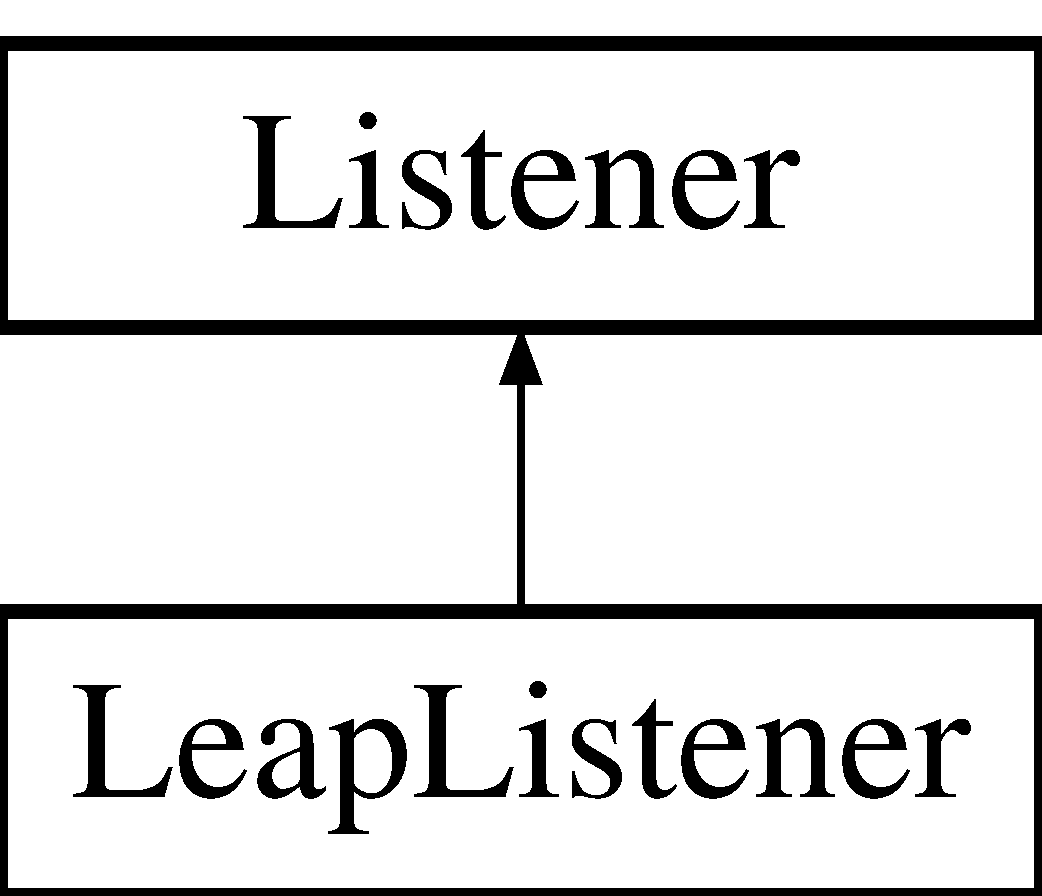
\includegraphics[height=2.000000cm]{classLeapListener}
\end{center}
\end{figure}
\subsection*{Public Member Functions}
\begin{DoxyCompactItemize}
\item 
Leap\+::\+Vector \hyperlink{classLeapListener_ac33a478bf23609d90da987045e6c09a6}{get\+Hand\+Direction} ()
\item 
Leap\+::\+Hand\+List \hyperlink{classLeapListener_a2926ac8cb2f4c2dc609224b72027d943}{get\+Hands\+List} ()
\item 
Leap\+::\+Vector \hyperlink{classLeapListener_ab7984ae05e41da2d31094488fc48d9cc}{get\+Leap\+Translation} ()
\item 
Leap\+::\+Vector \hyperlink{classLeapListener_ab247950ad2d43f8a86e8e1268b944391}{get\+Palm\+Normal} ()
\item 
virtual void \hyperlink{classLeapListener_a7d3131cb9c68b08adbecfa0991ef92f3}{on\+Connect} (const Leap\+::\+Controller \&)
\item 
virtual void \hyperlink{classLeapListener_a5b642ad6f373498b8cec2967d0931391}{on\+Disconnect} (const Leap\+::\+Controller \&)
\item 
virtual void \hyperlink{classLeapListener_a81f0ecbd8f407095abf359c30e8fa19e}{on\+Exit} (const Leap\+::\+Controller \&)
\item 
virtual void \hyperlink{classLeapListener_a63c3c85769306c066207fd00c7dbcf45}{on\+Frame} (const Leap\+::\+Controller \&)
\item 
virtual void \hyperlink{classLeapListener_a4eb09ec0bd5faf4ffd496d360aa7f1a4}{on\+Init} (const Leap\+::\+Controller \&)
\item 
virtual void \hyperlink{classLeapListener_ae4f8be9b6955e1f4ac4710f28dd70bd7}{on\+Service\+Connect} (const Leap\+::\+Controller \&)
\item 
virtual void \hyperlink{classLeapListener_ae63c5043bda6a559fe045c23fad2d58d}{on\+Service\+Disconnect} (const Leap\+::\+Controller \&)
\end{DoxyCompactItemize}
\subsection*{Private Attributes}
\begin{DoxyCompactItemize}
\item 
Leap\+::\+Arm \hyperlink{classLeapListener_adfad4850146dbbf8f098f53e540d2afc}{arm}
\item 
Leap\+::\+Frame \hyperlink{classLeapListener_a64eb85f79e30335bfb863ab0e5e0e524}{current\+Frame}
\item 
Leap\+::\+Finger\+List \hyperlink{classLeapListener_a5a04519bc2603793328375ad5e049773}{fingers}
\item 
Leap\+::\+Gesture\+List \hyperlink{classLeapListener_a724e5b46ff12f8982cbc4c378cfc7323}{gestures}
\item 
Leap\+::\+Vector \hyperlink{classLeapListener_ad8458a1467b2909621a4b1f116a4b5be}{hand\+Direction}
\item 
Leap\+::\+Hand\+List \hyperlink{classLeapListener_ac01cc7c1b36a473a942842b6068a8bc1}{hands}
\item 
Leap\+::\+Vector \hyperlink{classLeapListener_a31f0ee8db7d3954d0b2a7cc7c6cd5670}{leap\+Translation}
\item 
Leap\+::\+Vector \hyperlink{classLeapListener_ae084bdb6078ae06576cc4b6e678ed094}{palm\+Normal}
\item 
Leap\+::\+Frame \hyperlink{classLeapListener_a9182964b8502db776d1125fbb843a2a8}{previous\+Frame}
\end{DoxyCompactItemize}


\subsection{Detailed Description}
To handle Leap Motion events, create an instance of a Listener subclass and assign it to the Controller instance. The Controller calls the relevant Listener callback function when an event occurs, passing in a reference to itself. You do not have to implement callbacks for events you do not want to handle.

The Controller object calls these Listener functions from a thread created by the Leap Motion library, not the thread used to create or set the Listener instance. 

\subsection{Member Function Documentation}
\index{Leap\+Listener@{Leap\+Listener}!get\+Hand\+Direction@{get\+Hand\+Direction}}
\index{get\+Hand\+Direction@{get\+Hand\+Direction}!Leap\+Listener@{Leap\+Listener}}
\subsubsection[{\texorpdfstring{get\+Hand\+Direction()}{getHandDirection()}}]{\setlength{\rightskip}{0pt plus 5cm}Leap\+::\+Vector Leap\+Listener\+::get\+Hand\+Direction (
\begin{DoxyParamCaption}
{}
\end{DoxyParamCaption}
)}\hypertarget{classLeapListener_ac33a478bf23609d90da987045e6c09a6}{}\label{classLeapListener_ac33a478bf23609d90da987045e6c09a6}
Returns the direction from the palm position toward the fingers.

The direction is expressed as a unit vector pointing in the same direction as the directed line from the palm position to the fingers.

You can use the palm direction vector to compute the pitch and and yaw angles of the palm with respect to the horizontal plane. \index{Leap\+Listener@{Leap\+Listener}!get\+Hands\+List@{get\+Hands\+List}}
\index{get\+Hands\+List@{get\+Hands\+List}!Leap\+Listener@{Leap\+Listener}}
\subsubsection[{\texorpdfstring{get\+Hands\+List()}{getHandsList()}}]{\setlength{\rightskip}{0pt plus 5cm}Leap\+::\+Hand\+List Leap\+Listener\+::get\+Hands\+List (
\begin{DoxyParamCaption}
{}
\end{DoxyParamCaption}
)}\hypertarget{classLeapListener_a2926ac8cb2f4c2dc609224b72027d943}{}\label{classLeapListener_a2926ac8cb2f4c2dc609224b72027d943}
Returns the list of Hand objects detected in the frame.

The Hand\+List class acts like a vector-\/style array and supports iterators. You cannot remove or alter the member objects of a hand lists received from the Leap Motion A\+PI, but you can combine lists of the same object type.

The Hand\+List class defines additional functions for getting a member of the list based on its relative position within the Leap coordinate system. These functions include leftmost(), rightmost(), and frontmost(). \index{Leap\+Listener@{Leap\+Listener}!get\+Leap\+Translation@{get\+Leap\+Translation}}
\index{get\+Leap\+Translation@{get\+Leap\+Translation}!Leap\+Listener@{Leap\+Listener}}
\subsubsection[{\texorpdfstring{get\+Leap\+Translation()}{getLeapTranslation()}}]{\setlength{\rightskip}{0pt plus 5cm}Leap\+::\+Vector Leap\+Listener\+::get\+Leap\+Translation (
\begin{DoxyParamCaption}
{}
\end{DoxyParamCaption}
)}\hypertarget{classLeapListener_ab7984ae05e41da2d31094488fc48d9cc}{}\label{classLeapListener_ab7984ae05e41da2d31094488fc48d9cc}
Returns the change of position derived from the overall linear motion between the current frame and the specified frame. The returned translation vector provides the magnitude and direction of the movement in millimeters.

The Leap Motion software derives frame translation from the linear motion of all objects detected in the field of view.

If either the current or the previous frame is an invalid Frame object, then this method returns a zero vector. \index{Leap\+Listener@{Leap\+Listener}!get\+Palm\+Normal@{get\+Palm\+Normal}}
\index{get\+Palm\+Normal@{get\+Palm\+Normal}!Leap\+Listener@{Leap\+Listener}}
\subsubsection[{\texorpdfstring{get\+Palm\+Normal()}{getPalmNormal()}}]{\setlength{\rightskip}{0pt plus 5cm}Leap\+::\+Vector Leap\+Listener\+::get\+Palm\+Normal (
\begin{DoxyParamCaption}
{}
\end{DoxyParamCaption}
)}\hypertarget{classLeapListener_ab247950ad2d43f8a86e8e1268b944391}{}\label{classLeapListener_ab247950ad2d43f8a86e8e1268b944391}
Returns the normal vector to the palm.

If your hand is flat, this vector will point downward, or “out” of the front surface of your palm.

The direction is expressed as a unit vector pointing in the same direction as the palm normal (that is, a vector orthogonal to the palm).

You can use the palm normal vector to compute the roll angle of the palm with respect to the horizontal plane. \index{Leap\+Listener@{Leap\+Listener}!on\+Connect@{on\+Connect}}
\index{on\+Connect@{on\+Connect}!Leap\+Listener@{Leap\+Listener}}
\subsubsection[{\texorpdfstring{on\+Connect(const Leap\+::\+Controller \&)}{onConnect(const Leap::Controller &)}}]{\setlength{\rightskip}{0pt plus 5cm}virtual void Leap\+Listener\+::on\+Connect (
\begin{DoxyParamCaption}
\item[{const Leap\+::\+Controller \&}]{}
\end{DoxyParamCaption}
)\hspace{0.3cm}{\ttfamily [virtual]}}\hypertarget{classLeapListener_a7d3131cb9c68b08adbecfa0991ef92f3}{}\label{classLeapListener_a7d3131cb9c68b08adbecfa0991ef92f3}
Called when the Controller object connects to the Leap Motion software and the Leap Motion hardware device is plugged in, or when this Listener object is added to a Controller that is already connected. \index{Leap\+Listener@{Leap\+Listener}!on\+Disconnect@{on\+Disconnect}}
\index{on\+Disconnect@{on\+Disconnect}!Leap\+Listener@{Leap\+Listener}}
\subsubsection[{\texorpdfstring{on\+Disconnect(const Leap\+::\+Controller \&)}{onDisconnect(const Leap::Controller &)}}]{\setlength{\rightskip}{0pt plus 5cm}virtual void Leap\+Listener\+::on\+Disconnect (
\begin{DoxyParamCaption}
\item[{const Leap\+::\+Controller \&}]{}
\end{DoxyParamCaption}
)\hspace{0.3cm}{\ttfamily [virtual]}}\hypertarget{classLeapListener_a5b642ad6f373498b8cec2967d0931391}{}\label{classLeapListener_a5b642ad6f373498b8cec2967d0931391}
Called when the Controller object disconnects from the Leap Motion software or the Leap Motion hardware is unplugged.

The controller can disconnect when the Leap Motion device is unplugged, the user shuts the Leap Motion software down, or the Leap Motion software encounters an unrecoverable error. \index{Leap\+Listener@{Leap\+Listener}!on\+Exit@{on\+Exit}}
\index{on\+Exit@{on\+Exit}!Leap\+Listener@{Leap\+Listener}}
\subsubsection[{\texorpdfstring{on\+Exit(const Leap\+::\+Controller \&)}{onExit(const Leap::Controller &)}}]{\setlength{\rightskip}{0pt plus 5cm}virtual void Leap\+Listener\+::on\+Exit (
\begin{DoxyParamCaption}
\item[{const Leap\+::\+Controller \&}]{}
\end{DoxyParamCaption}
)\hspace{0.3cm}{\ttfamily [virtual]}}\hypertarget{classLeapListener_a81f0ecbd8f407095abf359c30e8fa19e}{}\label{classLeapListener_a81f0ecbd8f407095abf359c30e8fa19e}
Called when this Listener object is removed from the Controller or the Controller instance is destroyed. \index{Leap\+Listener@{Leap\+Listener}!on\+Frame@{on\+Frame}}
\index{on\+Frame@{on\+Frame}!Leap\+Listener@{Leap\+Listener}}
\subsubsection[{\texorpdfstring{on\+Frame(const Leap\+::\+Controller \&)}{onFrame(const Leap::Controller &)}}]{\setlength{\rightskip}{0pt plus 5cm}virtual void Leap\+Listener\+::on\+Frame (
\begin{DoxyParamCaption}
\item[{const Leap\+::\+Controller \&}]{}
\end{DoxyParamCaption}
)\hspace{0.3cm}{\ttfamily [virtual]}}\hypertarget{classLeapListener_a63c3c85769306c066207fd00c7dbcf45}{}\label{classLeapListener_a63c3c85769306c066207fd00c7dbcf45}
Called when a new frame of hand and finger tracking data is available. Access the new frame data using the Controller\+::frame() function.

Note, the Controller skips any pending on\+Frame events while your on\+Frame handler executes. If your implementation takes too long to return, one or more frames can be skipped. The Controller still inserts the skipped frames into the frame history. You can access recent frames by setting the history parameter when calling the Controller\+::frame() function. You can determine if any pending on\+Frame events were skipped by comparing the ID of the most recent frame with the ID of the last received frame. \index{Leap\+Listener@{Leap\+Listener}!on\+Init@{on\+Init}}
\index{on\+Init@{on\+Init}!Leap\+Listener@{Leap\+Listener}}
\subsubsection[{\texorpdfstring{on\+Init(const Leap\+::\+Controller \&)}{onInit(const Leap::Controller &)}}]{\setlength{\rightskip}{0pt plus 5cm}virtual void Leap\+Listener\+::on\+Init (
\begin{DoxyParamCaption}
\item[{const Leap\+::\+Controller \&}]{}
\end{DoxyParamCaption}
)\hspace{0.3cm}{\ttfamily [virtual]}}\hypertarget{classLeapListener_a4eb09ec0bd5faf4ffd496d360aa7f1a4}{}\label{classLeapListener_a4eb09ec0bd5faf4ffd496d360aa7f1a4}
Called once, when this Listener object is newly added to a Controller. \index{Leap\+Listener@{Leap\+Listener}!on\+Service\+Connect@{on\+Service\+Connect}}
\index{on\+Service\+Connect@{on\+Service\+Connect}!Leap\+Listener@{Leap\+Listener}}
\subsubsection[{\texorpdfstring{on\+Service\+Connect(const Leap\+::\+Controller \&)}{onServiceConnect(const Leap::Controller &)}}]{\setlength{\rightskip}{0pt plus 5cm}virtual void Leap\+Listener\+::on\+Service\+Connect (
\begin{DoxyParamCaption}
\item[{const Leap\+::\+Controller \&}]{}
\end{DoxyParamCaption}
)\hspace{0.3cm}{\ttfamily [virtual]}}\hypertarget{classLeapListener_ae4f8be9b6955e1f4ac4710f28dd70bd7}{}\label{classLeapListener_ae4f8be9b6955e1f4ac4710f28dd70bd7}
Called when the Leap Motion daemon/service connects to your application Controller. \index{Leap\+Listener@{Leap\+Listener}!on\+Service\+Disconnect@{on\+Service\+Disconnect}}
\index{on\+Service\+Disconnect@{on\+Service\+Disconnect}!Leap\+Listener@{Leap\+Listener}}
\subsubsection[{\texorpdfstring{on\+Service\+Disconnect(const Leap\+::\+Controller \&)}{onServiceDisconnect(const Leap::Controller &)}}]{\setlength{\rightskip}{0pt plus 5cm}virtual void Leap\+Listener\+::on\+Service\+Disconnect (
\begin{DoxyParamCaption}
\item[{const Leap\+::\+Controller \&}]{}
\end{DoxyParamCaption}
)\hspace{0.3cm}{\ttfamily [virtual]}}\hypertarget{classLeapListener_ae63c5043bda6a559fe045c23fad2d58d}{}\label{classLeapListener_ae63c5043bda6a559fe045c23fad2d58d}
Called if the Leap Motion daemon/service disconnects from your application Controller.

Normally, this callback is not invoked. It is only called if some external event or problem shuts down the service or otherwise interrupts the connection. 

\subsection{Field Documentation}
\index{Leap\+Listener@{Leap\+Listener}!arm@{arm}}
\index{arm@{arm}!Leap\+Listener@{Leap\+Listener}}
\subsubsection[{\texorpdfstring{arm}{arm}}]{\setlength{\rightskip}{0pt plus 5cm}Leap\+::\+Arm Leap\+Listener\+::arm\hspace{0.3cm}{\ttfamily [private]}}\hypertarget{classLeapListener_adfad4850146dbbf8f098f53e540d2afc}{}\label{classLeapListener_adfad4850146dbbf8f098f53e540d2afc}
The valid Arm object, which represents the forearm, obtained from a Hand object. \index{Leap\+Listener@{Leap\+Listener}!current\+Frame@{current\+Frame}}
\index{current\+Frame@{current\+Frame}!Leap\+Listener@{Leap\+Listener}}
\subsubsection[{\texorpdfstring{current\+Frame}{currentFrame}}]{\setlength{\rightskip}{0pt plus 5cm}Leap\+::\+Frame Leap\+Listener\+::current\+Frame\hspace{0.3cm}{\ttfamily [private]}}\hypertarget{classLeapListener_a64eb85f79e30335bfb863ab0e5e0e524}{}\label{classLeapListener_a64eb85f79e30335bfb863ab0e5e0e524}
The newest frame of tracking data from the Leap Motion software. \index{Leap\+Listener@{Leap\+Listener}!fingers@{fingers}}
\index{fingers@{fingers}!Leap\+Listener@{Leap\+Listener}}
\subsubsection[{\texorpdfstring{fingers}{fingers}}]{\setlength{\rightskip}{0pt plus 5cm}Leap\+::\+Finger\+List Leap\+Listener\+::fingers\hspace{0.3cm}{\ttfamily [private]}}\hypertarget{classLeapListener_a5a04519bc2603793328375ad5e049773}{}\label{classLeapListener_a5a04519bc2603793328375ad5e049773}
The Finger\+List containing all the tracked fingers in the current frame. \index{Leap\+Listener@{Leap\+Listener}!gestures@{gestures}}
\index{gestures@{gestures}!Leap\+Listener@{Leap\+Listener}}
\subsubsection[{\texorpdfstring{gestures}{gestures}}]{\setlength{\rightskip}{0pt plus 5cm}Leap\+::\+Gesture\+List Leap\+Listener\+::gestures\hspace{0.3cm}{\ttfamily [private]}}\hypertarget{classLeapListener_a724e5b46ff12f8982cbc4c378cfc7323}{}\label{classLeapListener_a724e5b46ff12f8982cbc4c378cfc7323}
The Gesture\+List containing all gestures that have occurred since the previous frame. \index{Leap\+Listener@{Leap\+Listener}!hand\+Direction@{hand\+Direction}}
\index{hand\+Direction@{hand\+Direction}!Leap\+Listener@{Leap\+Listener}}
\subsubsection[{\texorpdfstring{hand\+Direction}{handDirection}}]{\setlength{\rightskip}{0pt plus 5cm}Leap\+::\+Vector Leap\+Listener\+::hand\+Direction\hspace{0.3cm}{\ttfamily [private]}}\hypertarget{classLeapListener_ad8458a1467b2909621a4b1f116a4b5be}{}\label{classLeapListener_ad8458a1467b2909621a4b1f116a4b5be}
The direction from the palm position toward the fingers. \index{Leap\+Listener@{Leap\+Listener}!hands@{hands}}
\index{hands@{hands}!Leap\+Listener@{Leap\+Listener}}
\subsubsection[{\texorpdfstring{hands}{hands}}]{\setlength{\rightskip}{0pt plus 5cm}Leap\+::\+Hand\+List Leap\+Listener\+::hands\hspace{0.3cm}{\ttfamily [private]}}\hypertarget{classLeapListener_ac01cc7c1b36a473a942842b6068a8bc1}{}\label{classLeapListener_ac01cc7c1b36a473a942842b6068a8bc1}
The list of Hand objects detected in the frame. \index{Leap\+Listener@{Leap\+Listener}!leap\+Translation@{leap\+Translation}}
\index{leap\+Translation@{leap\+Translation}!Leap\+Listener@{Leap\+Listener}}
\subsubsection[{\texorpdfstring{leap\+Translation}{leapTranslation}}]{\setlength{\rightskip}{0pt plus 5cm}Leap\+::\+Vector Leap\+Listener\+::leap\+Translation\hspace{0.3cm}{\ttfamily [private]}}\hypertarget{classLeapListener_a31f0ee8db7d3954d0b2a7cc7c6cd5670}{}\label{classLeapListener_a31f0ee8db7d3954d0b2a7cc7c6cd5670}
The vector of translations occurred since the previous frame. \index{Leap\+Listener@{Leap\+Listener}!palm\+Normal@{palm\+Normal}}
\index{palm\+Normal@{palm\+Normal}!Leap\+Listener@{Leap\+Listener}}
\subsubsection[{\texorpdfstring{palm\+Normal}{palmNormal}}]{\setlength{\rightskip}{0pt plus 5cm}Leap\+::\+Vector Leap\+Listener\+::palm\+Normal\hspace{0.3cm}{\ttfamily [private]}}\hypertarget{classLeapListener_ae084bdb6078ae06576cc4b6e678ed094}{}\label{classLeapListener_ae084bdb6078ae06576cc4b6e678ed094}
The normal vector to the palm. \index{Leap\+Listener@{Leap\+Listener}!previous\+Frame@{previous\+Frame}}
\index{previous\+Frame@{previous\+Frame}!Leap\+Listener@{Leap\+Listener}}
\subsubsection[{\texorpdfstring{previous\+Frame}{previousFrame}}]{\setlength{\rightskip}{0pt plus 5cm}Leap\+::\+Frame Leap\+Listener\+::previous\+Frame\hspace{0.3cm}{\ttfamily [private]}}\hypertarget{classLeapListener_a9182964b8502db776d1125fbb843a2a8}{}\label{classLeapListener_a9182964b8502db776d1125fbb843a2a8}
The previous frame of tracking data from the Leap Motion software, retrieved in the stored frames by the controller. 

The documentation for this class was generated from the following file\+:\begin{DoxyCompactItemize}
\item 
\hyperlink{LeapListener_8h}{Leap\+Listener.\+h}\end{DoxyCompactItemize}

\hypertarget{classManager}{}\section{Manager Class Reference}
\label{classManager}\index{Manager@{Manager}}


{\ttfamily \#include $<$Manager.\+h$>$}

\subsection*{Public Member Functions}
\begin{DoxyCompactItemize}
\item 
\hyperlink{classManager_a1658ff9f18e38ccd9cb8b0b371b9c20b}{Manager} ()
\end{DoxyCompactItemize}
\subsection*{Private Member Functions}
\begin{DoxyCompactItemize}
\item 
void \hyperlink{classManager_a4c983bfe24e7bbda4126c674ec3b2bb7}{change\+Status} ()
\item 
void \hyperlink{classManager_abaf6f51c102571e1497bb616a10a34fe}{check\+Errors} ()
\item 
void \hyperlink{classManager_a4ddeea31257de952e0808827d777dbf6}{draw\+GL} ()
\item 
void \hyperlink{classManager_ac87bc79103e440a13485b005b09522c8}{draw\+Objects} (vector$<$ Drawable $\ast$ $>$ to\+Draw)
\item 
void \hyperlink{classManager_a5eea80bf7833673735c5287b3d3a41bf}{draw\+On} (vector$<$ Drawable $\ast$ $>$ to\+Draw)
\item 
void \hyperlink{classManager_a5e70b531d3af13c1a6af84dcc84fa225}{init} ()
\item 
void \hyperlink{classManager_aa30c66daa7d2e904f4b0cd2f2e6761a3}{init\+Leap} ()
\item 
void \hyperlink{classManager_a6a9eea3ca980647e117e1c9c7a682b0c}{init\+Myo} ()
\item 
mat4 \hyperlink{classManager_a280a961fb5889169708d838cde76e174}{leap\+Transform} (mat4 model\+Matrix)
\item 
void \hyperlink{classManager_a8abce1582047cb434a87dbe2dbe9c00d}{manage\+Bluetooth} ()
\item 
void \hyperlink{classManager_a366f9a671838a633672bc51f9d258646}{manage\+Games} ()
\item 
void \hyperlink{classManager_a98ffad2b354a12650d074e604edeffa6}{manage\+Menu} ()
\item 
void \hyperlink{classManager_af8645d966523587f7d7853e8a1497ed4}{manage\+Myo} ()
\item 
void \hyperlink{classManager_abaa47fce892b3e7cb91cce4f22f6dc2c}{manage\+Settings} ()
\item 
void \hyperlink{classManager_ad2a81bcf9fe948180aba898f2a177a39}{manage\+ThreeD} ()
\item 
void \hyperlink{classManager_a4c13c8264c0e9e02c9652d1350c69186}{manage\+Videos} ()
\item 
void \hyperlink{classManager_a30e2453a8522192bcf0061491fb0e768}{play\+Video} (sfe\+::\+Movie $\ast$movie)
\item 
void \hyperlink{classManager_af8c67c221068e4e3ccccf1d5f70ba8ee}{run} ()
\item 
void \hyperlink{classManager_ab9652f47f396c929f9b05b3619bd3254}{splash\+Screen} ()
\item 
void \hyperlink{classManager_a23be264535544bde00ce3b9216f5839e}{window\+Events} ()
\end{DoxyCompactItemize}
\subsection*{Private Attributes}
\begin{DoxyCompactItemize}
\item 
float \hyperlink{classManager_ac0797572bb4f1bccef22e3d5d09a7bb5}{angleX}
\item 
float \hyperlink{classManager_a4477aa8adddce16ff4cfb67b4c989ffe}{angleY}
\item 
float \hyperlink{classManager_ae82e575227f9f2fa73492d189fc3f1f0}{angleZ}
\item 
\hyperlink{classBluetooth}{Bluetooth} \hyperlink{classManager_a8ea668a9304bd75db548cb554e1938a0}{bluetooth}
\item 
Clock \hyperlink{classManager_a5a0b1978a70cd9f61dc0992f8d0ff1a7}{c\+Deb}
\item 
\hyperlink{Global_8h_a94049c48a0d77b80bca0fcb5b1281516}{M\+A\+N\+A\+G\+E\+R\+\_\+\+S\+T\+A\+T\+US} \hyperlink{classManager_a85a5040629f23c6cb6d722ff8b82d7d8}{current\+Status}
\item 
bool \hyperlink{classManager_a578fc01b433137173003b232fd5d8b5c}{draw\+With\+GL}
\item 
bool \hyperlink{classManager_a0f72e89b86fbe7d83006e33f3bf65af6}{enter\+Pressed}
\item 
bool \hyperlink{classManager_aa4d6ae86cd8a720763c6a65ec11ee4b2}{escape\+Pressed}
\item 
bool \hyperlink{classManager_a8244d18155248161add39e851a749009}{first\+Myo\+Pose}
\item 
bool \hyperlink{classManager_aa5b7a47a6fbe9ceeb794becfe4b5f783}{fullscreen}
\item 
float \hyperlink{classManager_a993a1557e2721396eec0c996875e7d7a}{height3D}
\item 
Hub $\ast$ \hyperlink{classManager_aa5b648bc7e8a1f5a667b7eaf3aa08152}{hub}
\item 
Leap\+::\+Controller \hyperlink{classManager_a98fbc2dcc62ae1c3f576cb85d5e331f4}{leap\+Controller}
\item 
\hyperlink{classLeapListener}{Leap\+Listener} \hyperlink{classManager_a34352d48738b796043dd3af2a447c5d3}{leap\+Listener}
\item 
bool \hyperlink{classManager_a0b7d7eef1b25676ff98d5cd037aaa9ac}{load\+Check}
\item 
\hyperlink{classMenu}{Menu} \hyperlink{classManager_ae849624e14738867ea9f6fcffef3da24}{menu}
\item 
Myo $\ast$ \hyperlink{classManager_a3764298317afa9f0e59e4366c1aac0a6}{myo\+Armband}
\item 
\hyperlink{classMyoConnector}{Myo\+Connector} \hyperlink{classManager_a8117b9ff0ea4c66e1379e088a6d28c5e}{myo\+Connector}
\item 
string \hyperlink{classManager_a86e49f5468df074459dfb578d1c24cfa}{myo\+Current\+Pose}
\item 
vec3 \hyperlink{classManager_a335d41f08d1075e7622a1caa64df2bdc}{myo\+Directions}
\item 
string \hyperlink{classManager_ac3e8cf065d787b8a79bd631dd54cfbc6}{myo\+Last\+Pose}
\item 
thread \hyperlink{classManager_a2b4f07b099ad6839729bd03bbeea52ad}{myo\+Manager}
\item 
\hyperlink{classSettings}{Settings} \hyperlink{classManager_a1799e8219d94565f72625e6821eda993}{settings}
\item 
Clock \hyperlink{classManager_a99819b2b5c34b66e76762ae20e6c6f55}{t\+Deb}
\item 
\hyperlink{classThreeD}{ThreeD} \hyperlink{classManager_aec79717dcdb413187e068925497eda32}{threeD}
\item 
\hyperlink{classVideo}{Video} \hyperlink{classManager_ab8b44618fbef7c927598d8154a5415de}{video}
\item 
float \hyperlink{classManager_a23e4b935abf9df5d71e5bf9dc89a9062}{V\+I\+E\+W\+\_\+\+D\+I\+M\+E\+N\+S\+I\+ON}
\item 
float \hyperlink{classManager_a835d170601628a807609db4f797c2382}{V\+I\+E\+W\+\_\+\+D\+I\+M\+E\+N\+S\+I\+O\+N\+\_\+X}
\item 
float \hyperlink{classManager_a2d875780ce3f0925ccd4165312600c06}{V\+I\+E\+W\+\_\+\+D\+I\+M\+E\+N\+S\+I\+O\+N\+\_\+Y}
\item 
float \hyperlink{classManager_aa1a80343a56401148926e13111041089}{V\+I\+E\+W\+\_\+\+P\+O\+S\+I\+T\+I\+O\+N\+\_\+\+B\+O\+T\+T\+O\+M\+\_\+X}
\item 
float \hyperlink{classManager_acccc2f78c0d94ca985fc83691daec707}{V\+I\+E\+W\+\_\+\+P\+O\+S\+I\+T\+I\+O\+N\+\_\+\+B\+O\+T\+T\+O\+M\+\_\+Y}
\item 
float \hyperlink{classManager_a48a66a40d7d6f25ca5373c104046e716}{V\+I\+E\+W\+\_\+\+P\+O\+S\+I\+T\+I\+O\+N\+\_\+\+L\+E\+F\+T\+\_\+X}
\item 
float \hyperlink{classManager_a30a44561824762281c6386bc8c395be1}{V\+I\+E\+W\+\_\+\+P\+O\+S\+I\+T\+I\+O\+N\+\_\+\+L\+E\+F\+T\+\_\+Y}
\item 
float \hyperlink{classManager_a186c67951bc370d8abcb7e4015dd8ff0}{V\+I\+E\+W\+\_\+\+P\+O\+S\+I\+T\+I\+O\+N\+\_\+\+R\+I\+G\+H\+T\+\_\+X}
\item 
float \hyperlink{classManager_a48eceb962e4626042d65dee9eb396afa}{V\+I\+E\+W\+\_\+\+P\+O\+S\+I\+T\+I\+O\+N\+\_\+\+R\+I\+G\+H\+T\+\_\+Y}
\item 
float \hyperlink{classManager_a6f253444bbaafa06701fda2d9cee9a29}{V\+I\+E\+W\+\_\+\+P\+O\+S\+I\+T\+I\+O\+N\+\_\+\+T\+O\+P\+\_\+X}
\item 
float \hyperlink{classManager_a5ebf3e78513ad3b4f53dd04554091c11}{V\+I\+E\+W\+\_\+\+P\+O\+S\+I\+T\+I\+O\+N\+\_\+\+T\+O\+P\+\_\+Y}
\item 
View \hyperlink{classManager_a1eeb8ba680636025d7b7c51cf5437bcd}{view\+Bottom}
\item 
float \hyperlink{classManager_aa8c3baaf60f70a4297c4f0dce0d07a7f}{view\+Height}
\item 
View \hyperlink{classManager_a554b1801bd4e3739883d2ab2515bc3bc}{view\+Left}
\item 
View \hyperlink{classManager_a053a04be419dfbf8c6ea09ca82f227b9}{view\+Right}
\item 
View \hyperlink{classManager_a2090b902817e39ca9d41955e6df815c0}{view\+Top}
\item 
float \hyperlink{classManager_a02b2d2ad1700f0791b74ae6b67c03f53}{view\+Width}
\item 
float \hyperlink{classManager_a6135e1c40a71a1bdbbbab15c84614de2}{width3D}
\item 
Render\+Window $\ast$ \hyperlink{classManager_a1ba39cb3b48db43ac88983af62d29ceb}{window}
\item 
float \hyperlink{classManager_a39946012d45458a913d1c1a4604be337}{zoom}
\end{DoxyCompactItemize}


\subsection{Constructor \& Destructor Documentation}
\index{Manager@{Manager}!Manager@{Manager}}
\index{Manager@{Manager}!Manager@{Manager}}
\subsubsection[{\texorpdfstring{Manager()}{Manager()}}]{\setlength{\rightskip}{0pt plus 5cm}Manager\+::\+Manager (
\begin{DoxyParamCaption}
{}
\end{DoxyParamCaption}
)}\hypertarget{classManager_a1658ff9f18e38ccd9cb8b0b371b9c20b}{}\label{classManager_a1658ff9f18e38ccd9cb8b0b371b9c20b}


\subsection{Member Function Documentation}
\index{Manager@{Manager}!change\+Status@{change\+Status}}
\index{change\+Status@{change\+Status}!Manager@{Manager}}
\subsubsection[{\texorpdfstring{change\+Status()}{changeStatus()}}]{\setlength{\rightskip}{0pt plus 5cm}void Manager\+::change\+Status (
\begin{DoxyParamCaption}
{}
\end{DoxyParamCaption}
)\hspace{0.3cm}{\ttfamily [private]}}\hypertarget{classManager_a4c983bfe24e7bbda4126c674ec3b2bb7}{}\label{classManager_a4c983bfe24e7bbda4126c674ec3b2bb7}
\index{Manager@{Manager}!check\+Errors@{check\+Errors}}
\index{check\+Errors@{check\+Errors}!Manager@{Manager}}
\subsubsection[{\texorpdfstring{check\+Errors()}{checkErrors()}}]{\setlength{\rightskip}{0pt plus 5cm}void Manager\+::check\+Errors (
\begin{DoxyParamCaption}
{}
\end{DoxyParamCaption}
)\hspace{0.3cm}{\ttfamily [private]}}\hypertarget{classManager_abaf6f51c102571e1497bb616a10a34fe}{}\label{classManager_abaf6f51c102571e1497bb616a10a34fe}
\index{Manager@{Manager}!draw\+GL@{draw\+GL}}
\index{draw\+GL@{draw\+GL}!Manager@{Manager}}
\subsubsection[{\texorpdfstring{draw\+G\+L()}{drawGL()}}]{\setlength{\rightskip}{0pt plus 5cm}void Manager\+::draw\+GL (
\begin{DoxyParamCaption}
{}
\end{DoxyParamCaption}
)\hspace{0.3cm}{\ttfamily [private]}}\hypertarget{classManager_a4ddeea31257de952e0808827d777dbf6}{}\label{classManager_a4ddeea31257de952e0808827d777dbf6}
\index{Manager@{Manager}!draw\+Objects@{draw\+Objects}}
\index{draw\+Objects@{draw\+Objects}!Manager@{Manager}}
\subsubsection[{\texorpdfstring{draw\+Objects(vector$<$ Drawable $\ast$ $>$ to\+Draw)}{drawObjects(vector< Drawable * > toDraw)}}]{\setlength{\rightskip}{0pt plus 5cm}void Manager\+::draw\+Objects (
\begin{DoxyParamCaption}
\item[{vector$<$ Drawable $\ast$ $>$}]{to\+Draw}
\end{DoxyParamCaption}
)\hspace{0.3cm}{\ttfamily [private]}}\hypertarget{classManager_ac87bc79103e440a13485b005b09522c8}{}\label{classManager_ac87bc79103e440a13485b005b09522c8}
\index{Manager@{Manager}!draw\+On@{draw\+On}}
\index{draw\+On@{draw\+On}!Manager@{Manager}}
\subsubsection[{\texorpdfstring{draw\+On(vector$<$ Drawable $\ast$ $>$ to\+Draw)}{drawOn(vector< Drawable * > toDraw)}}]{\setlength{\rightskip}{0pt plus 5cm}void Manager\+::draw\+On (
\begin{DoxyParamCaption}
\item[{vector$<$ Drawable $\ast$ $>$}]{to\+Draw}
\end{DoxyParamCaption}
)\hspace{0.3cm}{\ttfamily [private]}}\hypertarget{classManager_a5eea80bf7833673735c5287b3d3a41bf}{}\label{classManager_a5eea80bf7833673735c5287b3d3a41bf}
\index{Manager@{Manager}!init@{init}}
\index{init@{init}!Manager@{Manager}}
\subsubsection[{\texorpdfstring{init()}{init()}}]{\setlength{\rightskip}{0pt plus 5cm}void Manager\+::init (
\begin{DoxyParamCaption}
{}
\end{DoxyParamCaption}
)\hspace{0.3cm}{\ttfamily [private]}}\hypertarget{classManager_a5e70b531d3af13c1a6af84dcc84fa225}{}\label{classManager_a5e70b531d3af13c1a6af84dcc84fa225}
\index{Manager@{Manager}!init\+Leap@{init\+Leap}}
\index{init\+Leap@{init\+Leap}!Manager@{Manager}}
\subsubsection[{\texorpdfstring{init\+Leap()}{initLeap()}}]{\setlength{\rightskip}{0pt plus 5cm}void Manager\+::init\+Leap (
\begin{DoxyParamCaption}
{}
\end{DoxyParamCaption}
)\hspace{0.3cm}{\ttfamily [private]}}\hypertarget{classManager_aa30c66daa7d2e904f4b0cd2f2e6761a3}{}\label{classManager_aa30c66daa7d2e904f4b0cd2f2e6761a3}
\index{Manager@{Manager}!init\+Myo@{init\+Myo}}
\index{init\+Myo@{init\+Myo}!Manager@{Manager}}
\subsubsection[{\texorpdfstring{init\+Myo()}{initMyo()}}]{\setlength{\rightskip}{0pt plus 5cm}void Manager\+::init\+Myo (
\begin{DoxyParamCaption}
{}
\end{DoxyParamCaption}
)\hspace{0.3cm}{\ttfamily [private]}}\hypertarget{classManager_a6a9eea3ca980647e117e1c9c7a682b0c}{}\label{classManager_a6a9eea3ca980647e117e1c9c7a682b0c}
\index{Manager@{Manager}!leap\+Transform@{leap\+Transform}}
\index{leap\+Transform@{leap\+Transform}!Manager@{Manager}}
\subsubsection[{\texorpdfstring{leap\+Transform(mat4 model\+Matrix)}{leapTransform(mat4 modelMatrix)}}]{\setlength{\rightskip}{0pt plus 5cm}mat4 Manager\+::leap\+Transform (
\begin{DoxyParamCaption}
\item[{mat4}]{model\+Matrix}
\end{DoxyParamCaption}
)\hspace{0.3cm}{\ttfamily [private]}}\hypertarget{classManager_a280a961fb5889169708d838cde76e174}{}\label{classManager_a280a961fb5889169708d838cde76e174}
\index{Manager@{Manager}!manage\+Bluetooth@{manage\+Bluetooth}}
\index{manage\+Bluetooth@{manage\+Bluetooth}!Manager@{Manager}}
\subsubsection[{\texorpdfstring{manage\+Bluetooth()}{manageBluetooth()}}]{\setlength{\rightskip}{0pt plus 5cm}void Manager\+::manage\+Bluetooth (
\begin{DoxyParamCaption}
{}
\end{DoxyParamCaption}
)\hspace{0.3cm}{\ttfamily [private]}}\hypertarget{classManager_a8abce1582047cb434a87dbe2dbe9c00d}{}\label{classManager_a8abce1582047cb434a87dbe2dbe9c00d}
\index{Manager@{Manager}!manage\+Games@{manage\+Games}}
\index{manage\+Games@{manage\+Games}!Manager@{Manager}}
\subsubsection[{\texorpdfstring{manage\+Games()}{manageGames()}}]{\setlength{\rightskip}{0pt plus 5cm}void Manager\+::manage\+Games (
\begin{DoxyParamCaption}
{}
\end{DoxyParamCaption}
)\hspace{0.3cm}{\ttfamily [private]}}\hypertarget{classManager_a366f9a671838a633672bc51f9d258646}{}\label{classManager_a366f9a671838a633672bc51f9d258646}
\index{Manager@{Manager}!manage\+Menu@{manage\+Menu}}
\index{manage\+Menu@{manage\+Menu}!Manager@{Manager}}
\subsubsection[{\texorpdfstring{manage\+Menu()}{manageMenu()}}]{\setlength{\rightskip}{0pt plus 5cm}void Manager\+::manage\+Menu (
\begin{DoxyParamCaption}
{}
\end{DoxyParamCaption}
)\hspace{0.3cm}{\ttfamily [private]}}\hypertarget{classManager_a98ffad2b354a12650d074e604edeffa6}{}\label{classManager_a98ffad2b354a12650d074e604edeffa6}
\index{Manager@{Manager}!manage\+Myo@{manage\+Myo}}
\index{manage\+Myo@{manage\+Myo}!Manager@{Manager}}
\subsubsection[{\texorpdfstring{manage\+Myo()}{manageMyo()}}]{\setlength{\rightskip}{0pt plus 5cm}void Manager\+::manage\+Myo (
\begin{DoxyParamCaption}
{}
\end{DoxyParamCaption}
)\hspace{0.3cm}{\ttfamily [private]}}\hypertarget{classManager_af8645d966523587f7d7853e8a1497ed4}{}\label{classManager_af8645d966523587f7d7853e8a1497ed4}
\index{Manager@{Manager}!manage\+Settings@{manage\+Settings}}
\index{manage\+Settings@{manage\+Settings}!Manager@{Manager}}
\subsubsection[{\texorpdfstring{manage\+Settings()}{manageSettings()}}]{\setlength{\rightskip}{0pt plus 5cm}void Manager\+::manage\+Settings (
\begin{DoxyParamCaption}
{}
\end{DoxyParamCaption}
)\hspace{0.3cm}{\ttfamily [private]}}\hypertarget{classManager_abaa47fce892b3e7cb91cce4f22f6dc2c}{}\label{classManager_abaa47fce892b3e7cb91cce4f22f6dc2c}
\index{Manager@{Manager}!manage\+ThreeD@{manage\+ThreeD}}
\index{manage\+ThreeD@{manage\+ThreeD}!Manager@{Manager}}
\subsubsection[{\texorpdfstring{manage\+Three\+D()}{manageThreeD()}}]{\setlength{\rightskip}{0pt plus 5cm}void Manager\+::manage\+ThreeD (
\begin{DoxyParamCaption}
{}
\end{DoxyParamCaption}
)\hspace{0.3cm}{\ttfamily [private]}}\hypertarget{classManager_ad2a81bcf9fe948180aba898f2a177a39}{}\label{classManager_ad2a81bcf9fe948180aba898f2a177a39}
\index{Manager@{Manager}!manage\+Videos@{manage\+Videos}}
\index{manage\+Videos@{manage\+Videos}!Manager@{Manager}}
\subsubsection[{\texorpdfstring{manage\+Videos()}{manageVideos()}}]{\setlength{\rightskip}{0pt plus 5cm}void Manager\+::manage\+Videos (
\begin{DoxyParamCaption}
{}
\end{DoxyParamCaption}
)\hspace{0.3cm}{\ttfamily [private]}}\hypertarget{classManager_a4c13c8264c0e9e02c9652d1350c69186}{}\label{classManager_a4c13c8264c0e9e02c9652d1350c69186}
\index{Manager@{Manager}!play\+Video@{play\+Video}}
\index{play\+Video@{play\+Video}!Manager@{Manager}}
\subsubsection[{\texorpdfstring{play\+Video(sfe\+::\+Movie $\ast$movie)}{playVideo(sfe::Movie *movie)}}]{\setlength{\rightskip}{0pt plus 5cm}void Manager\+::play\+Video (
\begin{DoxyParamCaption}
\item[{sfe\+::\+Movie $\ast$}]{movie}
\end{DoxyParamCaption}
)\hspace{0.3cm}{\ttfamily [private]}}\hypertarget{classManager_a30e2453a8522192bcf0061491fb0e768}{}\label{classManager_a30e2453a8522192bcf0061491fb0e768}
\index{Manager@{Manager}!run@{run}}
\index{run@{run}!Manager@{Manager}}
\subsubsection[{\texorpdfstring{run()}{run()}}]{\setlength{\rightskip}{0pt plus 5cm}void Manager\+::run (
\begin{DoxyParamCaption}
{}
\end{DoxyParamCaption}
)\hspace{0.3cm}{\ttfamily [private]}}\hypertarget{classManager_af8c67c221068e4e3ccccf1d5f70ba8ee}{}\label{classManager_af8c67c221068e4e3ccccf1d5f70ba8ee}
\index{Manager@{Manager}!splash\+Screen@{splash\+Screen}}
\index{splash\+Screen@{splash\+Screen}!Manager@{Manager}}
\subsubsection[{\texorpdfstring{splash\+Screen()}{splashScreen()}}]{\setlength{\rightskip}{0pt plus 5cm}void Manager\+::splash\+Screen (
\begin{DoxyParamCaption}
{}
\end{DoxyParamCaption}
)\hspace{0.3cm}{\ttfamily [private]}}\hypertarget{classManager_ab9652f47f396c929f9b05b3619bd3254}{}\label{classManager_ab9652f47f396c929f9b05b3619bd3254}
\index{Manager@{Manager}!window\+Events@{window\+Events}}
\index{window\+Events@{window\+Events}!Manager@{Manager}}
\subsubsection[{\texorpdfstring{window\+Events()}{windowEvents()}}]{\setlength{\rightskip}{0pt plus 5cm}void Manager\+::window\+Events (
\begin{DoxyParamCaption}
{}
\end{DoxyParamCaption}
)\hspace{0.3cm}{\ttfamily [private]}}\hypertarget{classManager_a23be264535544bde00ce3b9216f5839e}{}\label{classManager_a23be264535544bde00ce3b9216f5839e}


\subsection{Field Documentation}
\index{Manager@{Manager}!angleX@{angleX}}
\index{angleX@{angleX}!Manager@{Manager}}
\subsubsection[{\texorpdfstring{angleX}{angleX}}]{\setlength{\rightskip}{0pt plus 5cm}float Manager\+::angleX\hspace{0.3cm}{\ttfamily [private]}}\hypertarget{classManager_ac0797572bb4f1bccef22e3d5d09a7bb5}{}\label{classManager_ac0797572bb4f1bccef22e3d5d09a7bb5}
\index{Manager@{Manager}!angleY@{angleY}}
\index{angleY@{angleY}!Manager@{Manager}}
\subsubsection[{\texorpdfstring{angleY}{angleY}}]{\setlength{\rightskip}{0pt plus 5cm}float Manager\+::angleY\hspace{0.3cm}{\ttfamily [private]}}\hypertarget{classManager_a4477aa8adddce16ff4cfb67b4c989ffe}{}\label{classManager_a4477aa8adddce16ff4cfb67b4c989ffe}
\index{Manager@{Manager}!angleZ@{angleZ}}
\index{angleZ@{angleZ}!Manager@{Manager}}
\subsubsection[{\texorpdfstring{angleZ}{angleZ}}]{\setlength{\rightskip}{0pt plus 5cm}float Manager\+::angleZ\hspace{0.3cm}{\ttfamily [private]}}\hypertarget{classManager_ae82e575227f9f2fa73492d189fc3f1f0}{}\label{classManager_ae82e575227f9f2fa73492d189fc3f1f0}
\index{Manager@{Manager}!bluetooth@{bluetooth}}
\index{bluetooth@{bluetooth}!Manager@{Manager}}
\subsubsection[{\texorpdfstring{bluetooth}{bluetooth}}]{\setlength{\rightskip}{0pt plus 5cm}{\bf Bluetooth} Manager\+::bluetooth\hspace{0.3cm}{\ttfamily [private]}}\hypertarget{classManager_a8ea668a9304bd75db548cb554e1938a0}{}\label{classManager_a8ea668a9304bd75db548cb554e1938a0}
\index{Manager@{Manager}!c\+Deb@{c\+Deb}}
\index{c\+Deb@{c\+Deb}!Manager@{Manager}}
\subsubsection[{\texorpdfstring{c\+Deb}{cDeb}}]{\setlength{\rightskip}{0pt plus 5cm}Clock Manager\+::c\+Deb\hspace{0.3cm}{\ttfamily [private]}}\hypertarget{classManager_a5a0b1978a70cd9f61dc0992f8d0ff1a7}{}\label{classManager_a5a0b1978a70cd9f61dc0992f8d0ff1a7}
\index{Manager@{Manager}!current\+Status@{current\+Status}}
\index{current\+Status@{current\+Status}!Manager@{Manager}}
\subsubsection[{\texorpdfstring{current\+Status}{currentStatus}}]{\setlength{\rightskip}{0pt plus 5cm}{\bf M\+A\+N\+A\+G\+E\+R\+\_\+\+S\+T\+A\+T\+US} Manager\+::current\+Status\hspace{0.3cm}{\ttfamily [private]}}\hypertarget{classManager_a85a5040629f23c6cb6d722ff8b82d7d8}{}\label{classManager_a85a5040629f23c6cb6d722ff8b82d7d8}
\index{Manager@{Manager}!draw\+With\+GL@{draw\+With\+GL}}
\index{draw\+With\+GL@{draw\+With\+GL}!Manager@{Manager}}
\subsubsection[{\texorpdfstring{draw\+With\+GL}{drawWithGL}}]{\setlength{\rightskip}{0pt plus 5cm}bool Manager\+::draw\+With\+GL\hspace{0.3cm}{\ttfamily [private]}}\hypertarget{classManager_a578fc01b433137173003b232fd5d8b5c}{}\label{classManager_a578fc01b433137173003b232fd5d8b5c}
\index{Manager@{Manager}!enter\+Pressed@{enter\+Pressed}}
\index{enter\+Pressed@{enter\+Pressed}!Manager@{Manager}}
\subsubsection[{\texorpdfstring{enter\+Pressed}{enterPressed}}]{\setlength{\rightskip}{0pt plus 5cm}bool Manager\+::enter\+Pressed\hspace{0.3cm}{\ttfamily [private]}}\hypertarget{classManager_a0f72e89b86fbe7d83006e33f3bf65af6}{}\label{classManager_a0f72e89b86fbe7d83006e33f3bf65af6}
\index{Manager@{Manager}!escape\+Pressed@{escape\+Pressed}}
\index{escape\+Pressed@{escape\+Pressed}!Manager@{Manager}}
\subsubsection[{\texorpdfstring{escape\+Pressed}{escapePressed}}]{\setlength{\rightskip}{0pt plus 5cm}bool Manager\+::escape\+Pressed\hspace{0.3cm}{\ttfamily [private]}}\hypertarget{classManager_aa4d6ae86cd8a720763c6a65ec11ee4b2}{}\label{classManager_aa4d6ae86cd8a720763c6a65ec11ee4b2}
\index{Manager@{Manager}!first\+Myo\+Pose@{first\+Myo\+Pose}}
\index{first\+Myo\+Pose@{first\+Myo\+Pose}!Manager@{Manager}}
\subsubsection[{\texorpdfstring{first\+Myo\+Pose}{firstMyoPose}}]{\setlength{\rightskip}{0pt plus 5cm}bool Manager\+::first\+Myo\+Pose\hspace{0.3cm}{\ttfamily [private]}}\hypertarget{classManager_a8244d18155248161add39e851a749009}{}\label{classManager_a8244d18155248161add39e851a749009}
\index{Manager@{Manager}!fullscreen@{fullscreen}}
\index{fullscreen@{fullscreen}!Manager@{Manager}}
\subsubsection[{\texorpdfstring{fullscreen}{fullscreen}}]{\setlength{\rightskip}{0pt plus 5cm}bool Manager\+::fullscreen\hspace{0.3cm}{\ttfamily [private]}}\hypertarget{classManager_aa5b7a47a6fbe9ceeb794becfe4b5f783}{}\label{classManager_aa5b7a47a6fbe9ceeb794becfe4b5f783}
\index{Manager@{Manager}!height3D@{height3D}}
\index{height3D@{height3D}!Manager@{Manager}}
\subsubsection[{\texorpdfstring{height3D}{height3D}}]{\setlength{\rightskip}{0pt plus 5cm}float Manager\+::height3D\hspace{0.3cm}{\ttfamily [private]}}\hypertarget{classManager_a993a1557e2721396eec0c996875e7d7a}{}\label{classManager_a993a1557e2721396eec0c996875e7d7a}
\index{Manager@{Manager}!hub@{hub}}
\index{hub@{hub}!Manager@{Manager}}
\subsubsection[{\texorpdfstring{hub}{hub}}]{\setlength{\rightskip}{0pt plus 5cm}Hub$\ast$ Manager\+::hub\hspace{0.3cm}{\ttfamily [private]}}\hypertarget{classManager_aa5b648bc7e8a1f5a667b7eaf3aa08152}{}\label{classManager_aa5b648bc7e8a1f5a667b7eaf3aa08152}
\index{Manager@{Manager}!leap\+Controller@{leap\+Controller}}
\index{leap\+Controller@{leap\+Controller}!Manager@{Manager}}
\subsubsection[{\texorpdfstring{leap\+Controller}{leapController}}]{\setlength{\rightskip}{0pt plus 5cm}Leap\+::\+Controller Manager\+::leap\+Controller\hspace{0.3cm}{\ttfamily [private]}}\hypertarget{classManager_a98fbc2dcc62ae1c3f576cb85d5e331f4}{}\label{classManager_a98fbc2dcc62ae1c3f576cb85d5e331f4}
\index{Manager@{Manager}!leap\+Listener@{leap\+Listener}}
\index{leap\+Listener@{leap\+Listener}!Manager@{Manager}}
\subsubsection[{\texorpdfstring{leap\+Listener}{leapListener}}]{\setlength{\rightskip}{0pt plus 5cm}{\bf Leap\+Listener} Manager\+::leap\+Listener\hspace{0.3cm}{\ttfamily [private]}}\hypertarget{classManager_a34352d48738b796043dd3af2a447c5d3}{}\label{classManager_a34352d48738b796043dd3af2a447c5d3}
\index{Manager@{Manager}!load\+Check@{load\+Check}}
\index{load\+Check@{load\+Check}!Manager@{Manager}}
\subsubsection[{\texorpdfstring{load\+Check}{loadCheck}}]{\setlength{\rightskip}{0pt plus 5cm}bool Manager\+::load\+Check\hspace{0.3cm}{\ttfamily [private]}}\hypertarget{classManager_a0b7d7eef1b25676ff98d5cd037aaa9ac}{}\label{classManager_a0b7d7eef1b25676ff98d5cd037aaa9ac}
\index{Manager@{Manager}!menu@{menu}}
\index{menu@{menu}!Manager@{Manager}}
\subsubsection[{\texorpdfstring{menu}{menu}}]{\setlength{\rightskip}{0pt plus 5cm}{\bf Menu} Manager\+::menu\hspace{0.3cm}{\ttfamily [private]}}\hypertarget{classManager_ae849624e14738867ea9f6fcffef3da24}{}\label{classManager_ae849624e14738867ea9f6fcffef3da24}
\index{Manager@{Manager}!myo\+Armband@{myo\+Armband}}
\index{myo\+Armband@{myo\+Armband}!Manager@{Manager}}
\subsubsection[{\texorpdfstring{myo\+Armband}{myoArmband}}]{\setlength{\rightskip}{0pt plus 5cm}Myo$\ast$ Manager\+::myo\+Armband\hspace{0.3cm}{\ttfamily [private]}}\hypertarget{classManager_a3764298317afa9f0e59e4366c1aac0a6}{}\label{classManager_a3764298317afa9f0e59e4366c1aac0a6}
\index{Manager@{Manager}!myo\+Connector@{myo\+Connector}}
\index{myo\+Connector@{myo\+Connector}!Manager@{Manager}}
\subsubsection[{\texorpdfstring{myo\+Connector}{myoConnector}}]{\setlength{\rightskip}{0pt plus 5cm}{\bf Myo\+Connector} Manager\+::myo\+Connector\hspace{0.3cm}{\ttfamily [private]}}\hypertarget{classManager_a8117b9ff0ea4c66e1379e088a6d28c5e}{}\label{classManager_a8117b9ff0ea4c66e1379e088a6d28c5e}
\index{Manager@{Manager}!myo\+Current\+Pose@{myo\+Current\+Pose}}
\index{myo\+Current\+Pose@{myo\+Current\+Pose}!Manager@{Manager}}
\subsubsection[{\texorpdfstring{myo\+Current\+Pose}{myoCurrentPose}}]{\setlength{\rightskip}{0pt plus 5cm}string Manager\+::myo\+Current\+Pose\hspace{0.3cm}{\ttfamily [private]}}\hypertarget{classManager_a86e49f5468df074459dfb578d1c24cfa}{}\label{classManager_a86e49f5468df074459dfb578d1c24cfa}
\index{Manager@{Manager}!myo\+Directions@{myo\+Directions}}
\index{myo\+Directions@{myo\+Directions}!Manager@{Manager}}
\subsubsection[{\texorpdfstring{myo\+Directions}{myoDirections}}]{\setlength{\rightskip}{0pt plus 5cm}vec3 Manager\+::myo\+Directions\hspace{0.3cm}{\ttfamily [private]}}\hypertarget{classManager_a335d41f08d1075e7622a1caa64df2bdc}{}\label{classManager_a335d41f08d1075e7622a1caa64df2bdc}
\index{Manager@{Manager}!myo\+Last\+Pose@{myo\+Last\+Pose}}
\index{myo\+Last\+Pose@{myo\+Last\+Pose}!Manager@{Manager}}
\subsubsection[{\texorpdfstring{myo\+Last\+Pose}{myoLastPose}}]{\setlength{\rightskip}{0pt plus 5cm}string Manager\+::myo\+Last\+Pose\hspace{0.3cm}{\ttfamily [private]}}\hypertarget{classManager_ac3e8cf065d787b8a79bd631dd54cfbc6}{}\label{classManager_ac3e8cf065d787b8a79bd631dd54cfbc6}
\index{Manager@{Manager}!myo\+Manager@{myo\+Manager}}
\index{myo\+Manager@{myo\+Manager}!Manager@{Manager}}
\subsubsection[{\texorpdfstring{myo\+Manager}{myoManager}}]{\setlength{\rightskip}{0pt plus 5cm}thread Manager\+::myo\+Manager\hspace{0.3cm}{\ttfamily [private]}}\hypertarget{classManager_a2b4f07b099ad6839729bd03bbeea52ad}{}\label{classManager_a2b4f07b099ad6839729bd03bbeea52ad}
\index{Manager@{Manager}!settings@{settings}}
\index{settings@{settings}!Manager@{Manager}}
\subsubsection[{\texorpdfstring{settings}{settings}}]{\setlength{\rightskip}{0pt plus 5cm}{\bf Settings} Manager\+::settings\hspace{0.3cm}{\ttfamily [private]}}\hypertarget{classManager_a1799e8219d94565f72625e6821eda993}{}\label{classManager_a1799e8219d94565f72625e6821eda993}
\index{Manager@{Manager}!t\+Deb@{t\+Deb}}
\index{t\+Deb@{t\+Deb}!Manager@{Manager}}
\subsubsection[{\texorpdfstring{t\+Deb}{tDeb}}]{\setlength{\rightskip}{0pt plus 5cm}Clock Manager\+::t\+Deb\hspace{0.3cm}{\ttfamily [private]}}\hypertarget{classManager_a99819b2b5c34b66e76762ae20e6c6f55}{}\label{classManager_a99819b2b5c34b66e76762ae20e6c6f55}
\index{Manager@{Manager}!threeD@{threeD}}
\index{threeD@{threeD}!Manager@{Manager}}
\subsubsection[{\texorpdfstring{threeD}{threeD}}]{\setlength{\rightskip}{0pt plus 5cm}{\bf ThreeD} Manager\+::threeD\hspace{0.3cm}{\ttfamily [private]}}\hypertarget{classManager_aec79717dcdb413187e068925497eda32}{}\label{classManager_aec79717dcdb413187e068925497eda32}
\index{Manager@{Manager}!video@{video}}
\index{video@{video}!Manager@{Manager}}
\subsubsection[{\texorpdfstring{video}{video}}]{\setlength{\rightskip}{0pt plus 5cm}{\bf Video} Manager\+::video\hspace{0.3cm}{\ttfamily [private]}}\hypertarget{classManager_ab8b44618fbef7c927598d8154a5415de}{}\label{classManager_ab8b44618fbef7c927598d8154a5415de}
\index{Manager@{Manager}!V\+I\+E\+W\+\_\+\+D\+I\+M\+E\+N\+S\+I\+ON@{V\+I\+E\+W\+\_\+\+D\+I\+M\+E\+N\+S\+I\+ON}}
\index{V\+I\+E\+W\+\_\+\+D\+I\+M\+E\+N\+S\+I\+ON@{V\+I\+E\+W\+\_\+\+D\+I\+M\+E\+N\+S\+I\+ON}!Manager@{Manager}}
\subsubsection[{\texorpdfstring{V\+I\+E\+W\+\_\+\+D\+I\+M\+E\+N\+S\+I\+ON}{VIEW_DIMENSION}}]{\setlength{\rightskip}{0pt plus 5cm}float Manager\+::\+V\+I\+E\+W\+\_\+\+D\+I\+M\+E\+N\+S\+I\+ON\hspace{0.3cm}{\ttfamily [private]}}\hypertarget{classManager_a23e4b935abf9df5d71e5bf9dc89a9062}{}\label{classManager_a23e4b935abf9df5d71e5bf9dc89a9062}
\index{Manager@{Manager}!V\+I\+E\+W\+\_\+\+D\+I\+M\+E\+N\+S\+I\+O\+N\+\_\+X@{V\+I\+E\+W\+\_\+\+D\+I\+M\+E\+N\+S\+I\+O\+N\+\_\+X}}
\index{V\+I\+E\+W\+\_\+\+D\+I\+M\+E\+N\+S\+I\+O\+N\+\_\+X@{V\+I\+E\+W\+\_\+\+D\+I\+M\+E\+N\+S\+I\+O\+N\+\_\+X}!Manager@{Manager}}
\subsubsection[{\texorpdfstring{V\+I\+E\+W\+\_\+\+D\+I\+M\+E\+N\+S\+I\+O\+N\+\_\+X}{VIEW_DIMENSION_X}}]{\setlength{\rightskip}{0pt plus 5cm}float Manager\+::\+V\+I\+E\+W\+\_\+\+D\+I\+M\+E\+N\+S\+I\+O\+N\+\_\+X\hspace{0.3cm}{\ttfamily [private]}}\hypertarget{classManager_a835d170601628a807609db4f797c2382}{}\label{classManager_a835d170601628a807609db4f797c2382}
\index{Manager@{Manager}!V\+I\+E\+W\+\_\+\+D\+I\+M\+E\+N\+S\+I\+O\+N\+\_\+Y@{V\+I\+E\+W\+\_\+\+D\+I\+M\+E\+N\+S\+I\+O\+N\+\_\+Y}}
\index{V\+I\+E\+W\+\_\+\+D\+I\+M\+E\+N\+S\+I\+O\+N\+\_\+Y@{V\+I\+E\+W\+\_\+\+D\+I\+M\+E\+N\+S\+I\+O\+N\+\_\+Y}!Manager@{Manager}}
\subsubsection[{\texorpdfstring{V\+I\+E\+W\+\_\+\+D\+I\+M\+E\+N\+S\+I\+O\+N\+\_\+Y}{VIEW_DIMENSION_Y}}]{\setlength{\rightskip}{0pt plus 5cm}float Manager\+::\+V\+I\+E\+W\+\_\+\+D\+I\+M\+E\+N\+S\+I\+O\+N\+\_\+Y\hspace{0.3cm}{\ttfamily [private]}}\hypertarget{classManager_a2d875780ce3f0925ccd4165312600c06}{}\label{classManager_a2d875780ce3f0925ccd4165312600c06}
\index{Manager@{Manager}!V\+I\+E\+W\+\_\+\+P\+O\+S\+I\+T\+I\+O\+N\+\_\+\+B\+O\+T\+T\+O\+M\+\_\+X@{V\+I\+E\+W\+\_\+\+P\+O\+S\+I\+T\+I\+O\+N\+\_\+\+B\+O\+T\+T\+O\+M\+\_\+X}}
\index{V\+I\+E\+W\+\_\+\+P\+O\+S\+I\+T\+I\+O\+N\+\_\+\+B\+O\+T\+T\+O\+M\+\_\+X@{V\+I\+E\+W\+\_\+\+P\+O\+S\+I\+T\+I\+O\+N\+\_\+\+B\+O\+T\+T\+O\+M\+\_\+X}!Manager@{Manager}}
\subsubsection[{\texorpdfstring{V\+I\+E\+W\+\_\+\+P\+O\+S\+I\+T\+I\+O\+N\+\_\+\+B\+O\+T\+T\+O\+M\+\_\+X}{VIEW_POSITION_BOTTOM_X}}]{\setlength{\rightskip}{0pt plus 5cm}float Manager\+::\+V\+I\+E\+W\+\_\+\+P\+O\+S\+I\+T\+I\+O\+N\+\_\+\+B\+O\+T\+T\+O\+M\+\_\+X\hspace{0.3cm}{\ttfamily [private]}}\hypertarget{classManager_aa1a80343a56401148926e13111041089}{}\label{classManager_aa1a80343a56401148926e13111041089}
\index{Manager@{Manager}!V\+I\+E\+W\+\_\+\+P\+O\+S\+I\+T\+I\+O\+N\+\_\+\+B\+O\+T\+T\+O\+M\+\_\+Y@{V\+I\+E\+W\+\_\+\+P\+O\+S\+I\+T\+I\+O\+N\+\_\+\+B\+O\+T\+T\+O\+M\+\_\+Y}}
\index{V\+I\+E\+W\+\_\+\+P\+O\+S\+I\+T\+I\+O\+N\+\_\+\+B\+O\+T\+T\+O\+M\+\_\+Y@{V\+I\+E\+W\+\_\+\+P\+O\+S\+I\+T\+I\+O\+N\+\_\+\+B\+O\+T\+T\+O\+M\+\_\+Y}!Manager@{Manager}}
\subsubsection[{\texorpdfstring{V\+I\+E\+W\+\_\+\+P\+O\+S\+I\+T\+I\+O\+N\+\_\+\+B\+O\+T\+T\+O\+M\+\_\+Y}{VIEW_POSITION_BOTTOM_Y}}]{\setlength{\rightskip}{0pt plus 5cm}float Manager\+::\+V\+I\+E\+W\+\_\+\+P\+O\+S\+I\+T\+I\+O\+N\+\_\+\+B\+O\+T\+T\+O\+M\+\_\+Y\hspace{0.3cm}{\ttfamily [private]}}\hypertarget{classManager_acccc2f78c0d94ca985fc83691daec707}{}\label{classManager_acccc2f78c0d94ca985fc83691daec707}
\index{Manager@{Manager}!V\+I\+E\+W\+\_\+\+P\+O\+S\+I\+T\+I\+O\+N\+\_\+\+L\+E\+F\+T\+\_\+X@{V\+I\+E\+W\+\_\+\+P\+O\+S\+I\+T\+I\+O\+N\+\_\+\+L\+E\+F\+T\+\_\+X}}
\index{V\+I\+E\+W\+\_\+\+P\+O\+S\+I\+T\+I\+O\+N\+\_\+\+L\+E\+F\+T\+\_\+X@{V\+I\+E\+W\+\_\+\+P\+O\+S\+I\+T\+I\+O\+N\+\_\+\+L\+E\+F\+T\+\_\+X}!Manager@{Manager}}
\subsubsection[{\texorpdfstring{V\+I\+E\+W\+\_\+\+P\+O\+S\+I\+T\+I\+O\+N\+\_\+\+L\+E\+F\+T\+\_\+X}{VIEW_POSITION_LEFT_X}}]{\setlength{\rightskip}{0pt plus 5cm}float Manager\+::\+V\+I\+E\+W\+\_\+\+P\+O\+S\+I\+T\+I\+O\+N\+\_\+\+L\+E\+F\+T\+\_\+X\hspace{0.3cm}{\ttfamily [private]}}\hypertarget{classManager_a48a66a40d7d6f25ca5373c104046e716}{}\label{classManager_a48a66a40d7d6f25ca5373c104046e716}
\index{Manager@{Manager}!V\+I\+E\+W\+\_\+\+P\+O\+S\+I\+T\+I\+O\+N\+\_\+\+L\+E\+F\+T\+\_\+Y@{V\+I\+E\+W\+\_\+\+P\+O\+S\+I\+T\+I\+O\+N\+\_\+\+L\+E\+F\+T\+\_\+Y}}
\index{V\+I\+E\+W\+\_\+\+P\+O\+S\+I\+T\+I\+O\+N\+\_\+\+L\+E\+F\+T\+\_\+Y@{V\+I\+E\+W\+\_\+\+P\+O\+S\+I\+T\+I\+O\+N\+\_\+\+L\+E\+F\+T\+\_\+Y}!Manager@{Manager}}
\subsubsection[{\texorpdfstring{V\+I\+E\+W\+\_\+\+P\+O\+S\+I\+T\+I\+O\+N\+\_\+\+L\+E\+F\+T\+\_\+Y}{VIEW_POSITION_LEFT_Y}}]{\setlength{\rightskip}{0pt plus 5cm}float Manager\+::\+V\+I\+E\+W\+\_\+\+P\+O\+S\+I\+T\+I\+O\+N\+\_\+\+L\+E\+F\+T\+\_\+Y\hspace{0.3cm}{\ttfamily [private]}}\hypertarget{classManager_a30a44561824762281c6386bc8c395be1}{}\label{classManager_a30a44561824762281c6386bc8c395be1}
\index{Manager@{Manager}!V\+I\+E\+W\+\_\+\+P\+O\+S\+I\+T\+I\+O\+N\+\_\+\+R\+I\+G\+H\+T\+\_\+X@{V\+I\+E\+W\+\_\+\+P\+O\+S\+I\+T\+I\+O\+N\+\_\+\+R\+I\+G\+H\+T\+\_\+X}}
\index{V\+I\+E\+W\+\_\+\+P\+O\+S\+I\+T\+I\+O\+N\+\_\+\+R\+I\+G\+H\+T\+\_\+X@{V\+I\+E\+W\+\_\+\+P\+O\+S\+I\+T\+I\+O\+N\+\_\+\+R\+I\+G\+H\+T\+\_\+X}!Manager@{Manager}}
\subsubsection[{\texorpdfstring{V\+I\+E\+W\+\_\+\+P\+O\+S\+I\+T\+I\+O\+N\+\_\+\+R\+I\+G\+H\+T\+\_\+X}{VIEW_POSITION_RIGHT_X}}]{\setlength{\rightskip}{0pt plus 5cm}float Manager\+::\+V\+I\+E\+W\+\_\+\+P\+O\+S\+I\+T\+I\+O\+N\+\_\+\+R\+I\+G\+H\+T\+\_\+X\hspace{0.3cm}{\ttfamily [private]}}\hypertarget{classManager_a186c67951bc370d8abcb7e4015dd8ff0}{}\label{classManager_a186c67951bc370d8abcb7e4015dd8ff0}
\index{Manager@{Manager}!V\+I\+E\+W\+\_\+\+P\+O\+S\+I\+T\+I\+O\+N\+\_\+\+R\+I\+G\+H\+T\+\_\+Y@{V\+I\+E\+W\+\_\+\+P\+O\+S\+I\+T\+I\+O\+N\+\_\+\+R\+I\+G\+H\+T\+\_\+Y}}
\index{V\+I\+E\+W\+\_\+\+P\+O\+S\+I\+T\+I\+O\+N\+\_\+\+R\+I\+G\+H\+T\+\_\+Y@{V\+I\+E\+W\+\_\+\+P\+O\+S\+I\+T\+I\+O\+N\+\_\+\+R\+I\+G\+H\+T\+\_\+Y}!Manager@{Manager}}
\subsubsection[{\texorpdfstring{V\+I\+E\+W\+\_\+\+P\+O\+S\+I\+T\+I\+O\+N\+\_\+\+R\+I\+G\+H\+T\+\_\+Y}{VIEW_POSITION_RIGHT_Y}}]{\setlength{\rightskip}{0pt plus 5cm}float Manager\+::\+V\+I\+E\+W\+\_\+\+P\+O\+S\+I\+T\+I\+O\+N\+\_\+\+R\+I\+G\+H\+T\+\_\+Y\hspace{0.3cm}{\ttfamily [private]}}\hypertarget{classManager_a48eceb962e4626042d65dee9eb396afa}{}\label{classManager_a48eceb962e4626042d65dee9eb396afa}
\index{Manager@{Manager}!V\+I\+E\+W\+\_\+\+P\+O\+S\+I\+T\+I\+O\+N\+\_\+\+T\+O\+P\+\_\+X@{V\+I\+E\+W\+\_\+\+P\+O\+S\+I\+T\+I\+O\+N\+\_\+\+T\+O\+P\+\_\+X}}
\index{V\+I\+E\+W\+\_\+\+P\+O\+S\+I\+T\+I\+O\+N\+\_\+\+T\+O\+P\+\_\+X@{V\+I\+E\+W\+\_\+\+P\+O\+S\+I\+T\+I\+O\+N\+\_\+\+T\+O\+P\+\_\+X}!Manager@{Manager}}
\subsubsection[{\texorpdfstring{V\+I\+E\+W\+\_\+\+P\+O\+S\+I\+T\+I\+O\+N\+\_\+\+T\+O\+P\+\_\+X}{VIEW_POSITION_TOP_X}}]{\setlength{\rightskip}{0pt plus 5cm}float Manager\+::\+V\+I\+E\+W\+\_\+\+P\+O\+S\+I\+T\+I\+O\+N\+\_\+\+T\+O\+P\+\_\+X\hspace{0.3cm}{\ttfamily [private]}}\hypertarget{classManager_a6f253444bbaafa06701fda2d9cee9a29}{}\label{classManager_a6f253444bbaafa06701fda2d9cee9a29}
\index{Manager@{Manager}!V\+I\+E\+W\+\_\+\+P\+O\+S\+I\+T\+I\+O\+N\+\_\+\+T\+O\+P\+\_\+Y@{V\+I\+E\+W\+\_\+\+P\+O\+S\+I\+T\+I\+O\+N\+\_\+\+T\+O\+P\+\_\+Y}}
\index{V\+I\+E\+W\+\_\+\+P\+O\+S\+I\+T\+I\+O\+N\+\_\+\+T\+O\+P\+\_\+Y@{V\+I\+E\+W\+\_\+\+P\+O\+S\+I\+T\+I\+O\+N\+\_\+\+T\+O\+P\+\_\+Y}!Manager@{Manager}}
\subsubsection[{\texorpdfstring{V\+I\+E\+W\+\_\+\+P\+O\+S\+I\+T\+I\+O\+N\+\_\+\+T\+O\+P\+\_\+Y}{VIEW_POSITION_TOP_Y}}]{\setlength{\rightskip}{0pt plus 5cm}float Manager\+::\+V\+I\+E\+W\+\_\+\+P\+O\+S\+I\+T\+I\+O\+N\+\_\+\+T\+O\+P\+\_\+Y\hspace{0.3cm}{\ttfamily [private]}}\hypertarget{classManager_a5ebf3e78513ad3b4f53dd04554091c11}{}\label{classManager_a5ebf3e78513ad3b4f53dd04554091c11}
\index{Manager@{Manager}!view\+Bottom@{view\+Bottom}}
\index{view\+Bottom@{view\+Bottom}!Manager@{Manager}}
\subsubsection[{\texorpdfstring{view\+Bottom}{viewBottom}}]{\setlength{\rightskip}{0pt plus 5cm}View Manager\+::view\+Bottom\hspace{0.3cm}{\ttfamily [private]}}\hypertarget{classManager_a1eeb8ba680636025d7b7c51cf5437bcd}{}\label{classManager_a1eeb8ba680636025d7b7c51cf5437bcd}
\index{Manager@{Manager}!view\+Height@{view\+Height}}
\index{view\+Height@{view\+Height}!Manager@{Manager}}
\subsubsection[{\texorpdfstring{view\+Height}{viewHeight}}]{\setlength{\rightskip}{0pt plus 5cm}float Manager\+::view\+Height\hspace{0.3cm}{\ttfamily [private]}}\hypertarget{classManager_aa8c3baaf60f70a4297c4f0dce0d07a7f}{}\label{classManager_aa8c3baaf60f70a4297c4f0dce0d07a7f}
\index{Manager@{Manager}!view\+Left@{view\+Left}}
\index{view\+Left@{view\+Left}!Manager@{Manager}}
\subsubsection[{\texorpdfstring{view\+Left}{viewLeft}}]{\setlength{\rightskip}{0pt plus 5cm}View Manager\+::view\+Left\hspace{0.3cm}{\ttfamily [private]}}\hypertarget{classManager_a554b1801bd4e3739883d2ab2515bc3bc}{}\label{classManager_a554b1801bd4e3739883d2ab2515bc3bc}
\index{Manager@{Manager}!view\+Right@{view\+Right}}
\index{view\+Right@{view\+Right}!Manager@{Manager}}
\subsubsection[{\texorpdfstring{view\+Right}{viewRight}}]{\setlength{\rightskip}{0pt plus 5cm}View Manager\+::view\+Right\hspace{0.3cm}{\ttfamily [private]}}\hypertarget{classManager_a053a04be419dfbf8c6ea09ca82f227b9}{}\label{classManager_a053a04be419dfbf8c6ea09ca82f227b9}
\index{Manager@{Manager}!view\+Top@{view\+Top}}
\index{view\+Top@{view\+Top}!Manager@{Manager}}
\subsubsection[{\texorpdfstring{view\+Top}{viewTop}}]{\setlength{\rightskip}{0pt plus 5cm}View Manager\+::view\+Top\hspace{0.3cm}{\ttfamily [private]}}\hypertarget{classManager_a2090b902817e39ca9d41955e6df815c0}{}\label{classManager_a2090b902817e39ca9d41955e6df815c0}
\index{Manager@{Manager}!view\+Width@{view\+Width}}
\index{view\+Width@{view\+Width}!Manager@{Manager}}
\subsubsection[{\texorpdfstring{view\+Width}{viewWidth}}]{\setlength{\rightskip}{0pt plus 5cm}float Manager\+::view\+Width\hspace{0.3cm}{\ttfamily [private]}}\hypertarget{classManager_a02b2d2ad1700f0791b74ae6b67c03f53}{}\label{classManager_a02b2d2ad1700f0791b74ae6b67c03f53}
\index{Manager@{Manager}!width3D@{width3D}}
\index{width3D@{width3D}!Manager@{Manager}}
\subsubsection[{\texorpdfstring{width3D}{width3D}}]{\setlength{\rightskip}{0pt plus 5cm}float Manager\+::width3D\hspace{0.3cm}{\ttfamily [private]}}\hypertarget{classManager_a6135e1c40a71a1bdbbbab15c84614de2}{}\label{classManager_a6135e1c40a71a1bdbbbab15c84614de2}
\index{Manager@{Manager}!window@{window}}
\index{window@{window}!Manager@{Manager}}
\subsubsection[{\texorpdfstring{window}{window}}]{\setlength{\rightskip}{0pt plus 5cm}Render\+Window$\ast$ Manager\+::window\hspace{0.3cm}{\ttfamily [private]}}\hypertarget{classManager_a1ba39cb3b48db43ac88983af62d29ceb}{}\label{classManager_a1ba39cb3b48db43ac88983af62d29ceb}
\index{Manager@{Manager}!zoom@{zoom}}
\index{zoom@{zoom}!Manager@{Manager}}
\subsubsection[{\texorpdfstring{zoom}{zoom}}]{\setlength{\rightskip}{0pt plus 5cm}float Manager\+::zoom\hspace{0.3cm}{\ttfamily [private]}}\hypertarget{classManager_a39946012d45458a913d1c1a4604be337}{}\label{classManager_a39946012d45458a913d1c1a4604be337}


The documentation for this class was generated from the following file\+:\begin{DoxyCompactItemize}
\item 
\hyperlink{Manager_8h}{Manager.\+h}\end{DoxyCompactItemize}

\hypertarget{classMenu}{}\section{Menu Class Reference}
\label{classMenu}\index{Menu@{Menu}}


{\ttfamily \#include $<$Menu.\+h$>$}

\subsection*{Public Member Functions}
\begin{DoxyCompactItemize}
\item 
\hyperlink{classMenu_ad466dd83355124a6ed958430450bfe94}{Menu} ()
\item 
void \hyperlink{classMenu_a0ab749d3c073f29d79070c4036aacf9d}{check\+Positions} ()
\item 
\hyperlink{Global_8h_a94049c48a0d77b80bca0fcb5b1281516}{M\+A\+N\+A\+G\+E\+R\+\_\+\+S\+T\+A\+T\+US} \hyperlink{classMenu_a2c11dd9aa1d02b232a2cd7d1b02d4790}{get\+Current\+Status} ()
\item 
bool \hyperlink{classMenu_aca94096321296262fe99d17d01556bad}{get\+Down\+Animation} ()
\item 
bool \hyperlink{classMenu_a2076597bda6ac7fcb654d19abc812a61}{get\+Left\+Animation} ()
\item 
vector$<$ Drawable $\ast$ $>$ \hyperlink{classMenu_a207642b71b3e74c8619f311e73eafffc}{get\+Objects\+Vector} ()
\item 
bool \hyperlink{classMenu_a114842e3e2fe84ca8ec08095dd08a92e}{get\+Right\+Animation} ()
\item 
bool \hyperlink{classMenu_a07c7b5c74648c47803ef1534b35c6584}{get\+Up\+Animation} ()
\item 
void \hyperlink{classMenu_a9a280ff90db10175b24a2d3d6515e3a8}{menu\+Events} ()
\item 
void \hyperlink{classMenu_aeebbcdcb7508e3cafc12ad1a32efc8e4}{set\+Down\+Animation} (bool \hyperlink{classMenu_aed34d6afbe07125d76062a534702cc96}{down\+Animation})
\item 
void \hyperlink{classMenu_a5b19e29c8681f88929c71d22a3327a0c}{set\+Left\+Animation} (bool \hyperlink{classMenu_a03bcd3608c9abd56b93c7ad12ee9a69e}{left\+Animation})
\item 
void \hyperlink{classMenu_aa5cd359d84a0296c42d099878410eeb8}{set\+Right\+Animation} (bool \hyperlink{classMenu_a8ce63316e4f8a2c57ca89e377ea7bb7d}{right\+Animation})
\item 
void \hyperlink{classMenu_ab94e0456a636056b422e4eb4b81aaf21}{set\+Up\+Animation} (bool \hyperlink{classMenu_add7681941b1c69a7ffd83838dfd0b308}{up\+Animation})
\end{DoxyCompactItemize}
\subsection*{Private Member Functions}
\begin{DoxyCompactItemize}
\item 
void \hyperlink{classMenu_a1345c7f2d610b7289e385031ab153c2a}{animate\+Down} ()
\item 
void \hyperlink{classMenu_a68cde302725490afd9e28673a525b48a}{animate\+Left} ()
\item 
void \hyperlink{classMenu_a3d5dd5c71d3985c4744a9147f623e77b}{animate\+Right} ()
\item 
void \hyperlink{classMenu_ad35665dbb77f3cbb1aa5fcdcb92ce39b}{animate\+Up} ()
\item 
void \hyperlink{classMenu_a342d2a526a850dbf2d1aecd830b91287}{init} ()
\item 
void \hyperlink{classMenu_a5b7ec5defefb42f3636ed019e42fd278}{set\+Positions} ()
\end{DoxyCompactItemize}
\subsection*{Private Attributes}
\begin{DoxyCompactItemize}
\item 
float \hyperlink{classMenu_ac2867e5a9ffe9ddc607410485fd0f245}{animation\+Speed}
\item 
float \hyperlink{classMenu_af32e0e46edcdc1003b350e8af243628a}{animation\+Time}
\item 
bool \hyperlink{classMenu_aed34d6afbe07125d76062a534702cc96}{down\+Animation}
\item 
bool \hyperlink{classMenu_a00fb6eae49e90e2d136acc30113a586d}{first}
\item 
int \hyperlink{classMenu_ae4477bba3eedd781a216463d426ccc0d}{first\+Text\+Position}
\item 
bool \hyperlink{classMenu_a03bcd3608c9abd56b93c7ad12ee9a69e}{left\+Animation}
\item 
int \hyperlink{classMenu_ae5530fcf346921fed30a419a162b3b1e}{left\+Position}
\item 
Font \hyperlink{classMenu_a42c864293b5786e44c41825a9f58a4d0}{menu\+Font}
\item 
vector$<$ Text $>$ \hyperlink{classMenu_a1aeea0f0b6990ce000cd25a15b5580fa}{menu\+Texts}
\item 
int \hyperlink{classMenu_af12ee21ad6f9d7f3da9573097eca8a84}{n\+Text}
\item 
int \hyperlink{classMenu_ae88d145e5fa875757702b497f0fc41c5}{out\+Position}
\item 
bool \hyperlink{classMenu_a8ce63316e4f8a2c57ca89e377ea7bb7d}{right\+Animation}
\item 
int \hyperlink{classMenu_ac164eee1fb3453d836d53eb59686ac32}{right\+Position}
\item 
float \hyperlink{classMenu_a3edde1cae9d582ce1521009d1744068d}{scale\+Factor}
\item 
vector$<$ float $>$ \hyperlink{classMenu_aca5731572596b8e5dbd962b41644ae27}{speeds}
\item 
int \hyperlink{classMenu_a7fc5cd2396e512ef71bb7c3d367710d7}{step\+Counter}
\item 
Rectangle\+Shape \hyperlink{classMenu_a56e4febfec0254757193602cabcb88e1}{strip}
\item 
unsigned int \hyperlink{classMenu_af50094c0a9831c625dc16a713652777c}{text\+Size}
\item 
vector$<$ Drawable $\ast$ $>$ \hyperlink{classMenu_ad64e0b08c47706709d3b23a61caf036f}{to\+Draw}
\item 
bool \hyperlink{classMenu_add7681941b1c69a7ffd83838dfd0b308}{up\+Animation}
\end{DoxyCompactItemize}


\subsection{Constructor \& Destructor Documentation}
\index{Menu@{Menu}!Menu@{Menu}}
\index{Menu@{Menu}!Menu@{Menu}}
\subsubsection[{\texorpdfstring{Menu()}{Menu()}}]{\setlength{\rightskip}{0pt plus 5cm}Menu\+::\+Menu (
\begin{DoxyParamCaption}
{}
\end{DoxyParamCaption}
)}\hypertarget{classMenu_ad466dd83355124a6ed958430450bfe94}{}\label{classMenu_ad466dd83355124a6ed958430450bfe94}


\subsection{Member Function Documentation}
\index{Menu@{Menu}!animate\+Down@{animate\+Down}}
\index{animate\+Down@{animate\+Down}!Menu@{Menu}}
\subsubsection[{\texorpdfstring{animate\+Down()}{animateDown()}}]{\setlength{\rightskip}{0pt plus 5cm}void Menu\+::animate\+Down (
\begin{DoxyParamCaption}
{}
\end{DoxyParamCaption}
)\hspace{0.3cm}{\ttfamily [private]}}\hypertarget{classMenu_a1345c7f2d610b7289e385031ab153c2a}{}\label{classMenu_a1345c7f2d610b7289e385031ab153c2a}
\index{Menu@{Menu}!animate\+Left@{animate\+Left}}
\index{animate\+Left@{animate\+Left}!Menu@{Menu}}
\subsubsection[{\texorpdfstring{animate\+Left()}{animateLeft()}}]{\setlength{\rightskip}{0pt plus 5cm}void Menu\+::animate\+Left (
\begin{DoxyParamCaption}
{}
\end{DoxyParamCaption}
)\hspace{0.3cm}{\ttfamily [private]}}\hypertarget{classMenu_a68cde302725490afd9e28673a525b48a}{}\label{classMenu_a68cde302725490afd9e28673a525b48a}
\index{Menu@{Menu}!animate\+Right@{animate\+Right}}
\index{animate\+Right@{animate\+Right}!Menu@{Menu}}
\subsubsection[{\texorpdfstring{animate\+Right()}{animateRight()}}]{\setlength{\rightskip}{0pt plus 5cm}void Menu\+::animate\+Right (
\begin{DoxyParamCaption}
{}
\end{DoxyParamCaption}
)\hspace{0.3cm}{\ttfamily [private]}}\hypertarget{classMenu_a3d5dd5c71d3985c4744a9147f623e77b}{}\label{classMenu_a3d5dd5c71d3985c4744a9147f623e77b}
\index{Menu@{Menu}!animate\+Up@{animate\+Up}}
\index{animate\+Up@{animate\+Up}!Menu@{Menu}}
\subsubsection[{\texorpdfstring{animate\+Up()}{animateUp()}}]{\setlength{\rightskip}{0pt plus 5cm}void Menu\+::animate\+Up (
\begin{DoxyParamCaption}
{}
\end{DoxyParamCaption}
)\hspace{0.3cm}{\ttfamily [private]}}\hypertarget{classMenu_ad35665dbb77f3cbb1aa5fcdcb92ce39b}{}\label{classMenu_ad35665dbb77f3cbb1aa5fcdcb92ce39b}
\index{Menu@{Menu}!check\+Positions@{check\+Positions}}
\index{check\+Positions@{check\+Positions}!Menu@{Menu}}
\subsubsection[{\texorpdfstring{check\+Positions()}{checkPositions()}}]{\setlength{\rightskip}{0pt plus 5cm}void Menu\+::check\+Positions (
\begin{DoxyParamCaption}
{}
\end{DoxyParamCaption}
)}\hypertarget{classMenu_a0ab749d3c073f29d79070c4036aacf9d}{}\label{classMenu_a0ab749d3c073f29d79070c4036aacf9d}
\index{Menu@{Menu}!get\+Current\+Status@{get\+Current\+Status}}
\index{get\+Current\+Status@{get\+Current\+Status}!Menu@{Menu}}
\subsubsection[{\texorpdfstring{get\+Current\+Status()}{getCurrentStatus()}}]{\setlength{\rightskip}{0pt plus 5cm}{\bf M\+A\+N\+A\+G\+E\+R\+\_\+\+S\+T\+A\+T\+US} Menu\+::get\+Current\+Status (
\begin{DoxyParamCaption}
{}
\end{DoxyParamCaption}
)}\hypertarget{classMenu_a2c11dd9aa1d02b232a2cd7d1b02d4790}{}\label{classMenu_a2c11dd9aa1d02b232a2cd7d1b02d4790}
\index{Menu@{Menu}!get\+Down\+Animation@{get\+Down\+Animation}}
\index{get\+Down\+Animation@{get\+Down\+Animation}!Menu@{Menu}}
\subsubsection[{\texorpdfstring{get\+Down\+Animation()}{getDownAnimation()}}]{\setlength{\rightskip}{0pt plus 5cm}bool Menu\+::get\+Down\+Animation (
\begin{DoxyParamCaption}
{}
\end{DoxyParamCaption}
)}\hypertarget{classMenu_aca94096321296262fe99d17d01556bad}{}\label{classMenu_aca94096321296262fe99d17d01556bad}
\index{Menu@{Menu}!get\+Left\+Animation@{get\+Left\+Animation}}
\index{get\+Left\+Animation@{get\+Left\+Animation}!Menu@{Menu}}
\subsubsection[{\texorpdfstring{get\+Left\+Animation()}{getLeftAnimation()}}]{\setlength{\rightskip}{0pt plus 5cm}bool Menu\+::get\+Left\+Animation (
\begin{DoxyParamCaption}
{}
\end{DoxyParamCaption}
)}\hypertarget{classMenu_a2076597bda6ac7fcb654d19abc812a61}{}\label{classMenu_a2076597bda6ac7fcb654d19abc812a61}
\index{Menu@{Menu}!get\+Objects\+Vector@{get\+Objects\+Vector}}
\index{get\+Objects\+Vector@{get\+Objects\+Vector}!Menu@{Menu}}
\subsubsection[{\texorpdfstring{get\+Objects\+Vector()}{getObjectsVector()}}]{\setlength{\rightskip}{0pt plus 5cm}vector$<$Drawable$\ast$$>$ Menu\+::get\+Objects\+Vector (
\begin{DoxyParamCaption}
{}
\end{DoxyParamCaption}
)}\hypertarget{classMenu_a207642b71b3e74c8619f311e73eafffc}{}\label{classMenu_a207642b71b3e74c8619f311e73eafffc}
\index{Menu@{Menu}!get\+Right\+Animation@{get\+Right\+Animation}}
\index{get\+Right\+Animation@{get\+Right\+Animation}!Menu@{Menu}}
\subsubsection[{\texorpdfstring{get\+Right\+Animation()}{getRightAnimation()}}]{\setlength{\rightskip}{0pt plus 5cm}bool Menu\+::get\+Right\+Animation (
\begin{DoxyParamCaption}
{}
\end{DoxyParamCaption}
)}\hypertarget{classMenu_a114842e3e2fe84ca8ec08095dd08a92e}{}\label{classMenu_a114842e3e2fe84ca8ec08095dd08a92e}
\index{Menu@{Menu}!get\+Up\+Animation@{get\+Up\+Animation}}
\index{get\+Up\+Animation@{get\+Up\+Animation}!Menu@{Menu}}
\subsubsection[{\texorpdfstring{get\+Up\+Animation()}{getUpAnimation()}}]{\setlength{\rightskip}{0pt plus 5cm}bool Menu\+::get\+Up\+Animation (
\begin{DoxyParamCaption}
{}
\end{DoxyParamCaption}
)}\hypertarget{classMenu_a07c7b5c74648c47803ef1534b35c6584}{}\label{classMenu_a07c7b5c74648c47803ef1534b35c6584}
\index{Menu@{Menu}!init@{init}}
\index{init@{init}!Menu@{Menu}}
\subsubsection[{\texorpdfstring{init()}{init()}}]{\setlength{\rightskip}{0pt plus 5cm}void Menu\+::init (
\begin{DoxyParamCaption}
{}
\end{DoxyParamCaption}
)\hspace{0.3cm}{\ttfamily [private]}}\hypertarget{classMenu_a342d2a526a850dbf2d1aecd830b91287}{}\label{classMenu_a342d2a526a850dbf2d1aecd830b91287}
\index{Menu@{Menu}!menu\+Events@{menu\+Events}}
\index{menu\+Events@{menu\+Events}!Menu@{Menu}}
\subsubsection[{\texorpdfstring{menu\+Events()}{menuEvents()}}]{\setlength{\rightskip}{0pt plus 5cm}void Menu\+::menu\+Events (
\begin{DoxyParamCaption}
{}
\end{DoxyParamCaption}
)}\hypertarget{classMenu_a9a280ff90db10175b24a2d3d6515e3a8}{}\label{classMenu_a9a280ff90db10175b24a2d3d6515e3a8}
\index{Menu@{Menu}!set\+Down\+Animation@{set\+Down\+Animation}}
\index{set\+Down\+Animation@{set\+Down\+Animation}!Menu@{Menu}}
\subsubsection[{\texorpdfstring{set\+Down\+Animation(bool down\+Animation)}{setDownAnimation(bool downAnimation)}}]{\setlength{\rightskip}{0pt plus 5cm}void Menu\+::set\+Down\+Animation (
\begin{DoxyParamCaption}
\item[{bool}]{down\+Animation}
\end{DoxyParamCaption}
)}\hypertarget{classMenu_aeebbcdcb7508e3cafc12ad1a32efc8e4}{}\label{classMenu_aeebbcdcb7508e3cafc12ad1a32efc8e4}
\index{Menu@{Menu}!set\+Left\+Animation@{set\+Left\+Animation}}
\index{set\+Left\+Animation@{set\+Left\+Animation}!Menu@{Menu}}
\subsubsection[{\texorpdfstring{set\+Left\+Animation(bool left\+Animation)}{setLeftAnimation(bool leftAnimation)}}]{\setlength{\rightskip}{0pt plus 5cm}void Menu\+::set\+Left\+Animation (
\begin{DoxyParamCaption}
\item[{bool}]{left\+Animation}
\end{DoxyParamCaption}
)}\hypertarget{classMenu_a5b19e29c8681f88929c71d22a3327a0c}{}\label{classMenu_a5b19e29c8681f88929c71d22a3327a0c}
\index{Menu@{Menu}!set\+Positions@{set\+Positions}}
\index{set\+Positions@{set\+Positions}!Menu@{Menu}}
\subsubsection[{\texorpdfstring{set\+Positions()}{setPositions()}}]{\setlength{\rightskip}{0pt plus 5cm}void Menu\+::set\+Positions (
\begin{DoxyParamCaption}
{}
\end{DoxyParamCaption}
)\hspace{0.3cm}{\ttfamily [private]}}\hypertarget{classMenu_a5b7ec5defefb42f3636ed019e42fd278}{}\label{classMenu_a5b7ec5defefb42f3636ed019e42fd278}
\index{Menu@{Menu}!set\+Right\+Animation@{set\+Right\+Animation}}
\index{set\+Right\+Animation@{set\+Right\+Animation}!Menu@{Menu}}
\subsubsection[{\texorpdfstring{set\+Right\+Animation(bool right\+Animation)}{setRightAnimation(bool rightAnimation)}}]{\setlength{\rightskip}{0pt plus 5cm}void Menu\+::set\+Right\+Animation (
\begin{DoxyParamCaption}
\item[{bool}]{right\+Animation}
\end{DoxyParamCaption}
)}\hypertarget{classMenu_aa5cd359d84a0296c42d099878410eeb8}{}\label{classMenu_aa5cd359d84a0296c42d099878410eeb8}
\index{Menu@{Menu}!set\+Up\+Animation@{set\+Up\+Animation}}
\index{set\+Up\+Animation@{set\+Up\+Animation}!Menu@{Menu}}
\subsubsection[{\texorpdfstring{set\+Up\+Animation(bool up\+Animation)}{setUpAnimation(bool upAnimation)}}]{\setlength{\rightskip}{0pt plus 5cm}void Menu\+::set\+Up\+Animation (
\begin{DoxyParamCaption}
\item[{bool}]{up\+Animation}
\end{DoxyParamCaption}
)}\hypertarget{classMenu_ab94e0456a636056b422e4eb4b81aaf21}{}\label{classMenu_ab94e0456a636056b422e4eb4b81aaf21}


\subsection{Field Documentation}
\index{Menu@{Menu}!animation\+Speed@{animation\+Speed}}
\index{animation\+Speed@{animation\+Speed}!Menu@{Menu}}
\subsubsection[{\texorpdfstring{animation\+Speed}{animationSpeed}}]{\setlength{\rightskip}{0pt plus 5cm}float Menu\+::animation\+Speed\hspace{0.3cm}{\ttfamily [private]}}\hypertarget{classMenu_ac2867e5a9ffe9ddc607410485fd0f245}{}\label{classMenu_ac2867e5a9ffe9ddc607410485fd0f245}
\index{Menu@{Menu}!animation\+Time@{animation\+Time}}
\index{animation\+Time@{animation\+Time}!Menu@{Menu}}
\subsubsection[{\texorpdfstring{animation\+Time}{animationTime}}]{\setlength{\rightskip}{0pt plus 5cm}float Menu\+::animation\+Time\hspace{0.3cm}{\ttfamily [private]}}\hypertarget{classMenu_af32e0e46edcdc1003b350e8af243628a}{}\label{classMenu_af32e0e46edcdc1003b350e8af243628a}
\index{Menu@{Menu}!down\+Animation@{down\+Animation}}
\index{down\+Animation@{down\+Animation}!Menu@{Menu}}
\subsubsection[{\texorpdfstring{down\+Animation}{downAnimation}}]{\setlength{\rightskip}{0pt plus 5cm}bool Menu\+::down\+Animation\hspace{0.3cm}{\ttfamily [private]}}\hypertarget{classMenu_aed34d6afbe07125d76062a534702cc96}{}\label{classMenu_aed34d6afbe07125d76062a534702cc96}
\index{Menu@{Menu}!first@{first}}
\index{first@{first}!Menu@{Menu}}
\subsubsection[{\texorpdfstring{first}{first}}]{\setlength{\rightskip}{0pt plus 5cm}bool Menu\+::first\hspace{0.3cm}{\ttfamily [private]}}\hypertarget{classMenu_a00fb6eae49e90e2d136acc30113a586d}{}\label{classMenu_a00fb6eae49e90e2d136acc30113a586d}
\index{Menu@{Menu}!first\+Text\+Position@{first\+Text\+Position}}
\index{first\+Text\+Position@{first\+Text\+Position}!Menu@{Menu}}
\subsubsection[{\texorpdfstring{first\+Text\+Position}{firstTextPosition}}]{\setlength{\rightskip}{0pt plus 5cm}int Menu\+::first\+Text\+Position\hspace{0.3cm}{\ttfamily [private]}}\hypertarget{classMenu_ae4477bba3eedd781a216463d426ccc0d}{}\label{classMenu_ae4477bba3eedd781a216463d426ccc0d}
\index{Menu@{Menu}!left\+Animation@{left\+Animation}}
\index{left\+Animation@{left\+Animation}!Menu@{Menu}}
\subsubsection[{\texorpdfstring{left\+Animation}{leftAnimation}}]{\setlength{\rightskip}{0pt plus 5cm}bool Menu\+::left\+Animation\hspace{0.3cm}{\ttfamily [private]}}\hypertarget{classMenu_a03bcd3608c9abd56b93c7ad12ee9a69e}{}\label{classMenu_a03bcd3608c9abd56b93c7ad12ee9a69e}
\index{Menu@{Menu}!left\+Position@{left\+Position}}
\index{left\+Position@{left\+Position}!Menu@{Menu}}
\subsubsection[{\texorpdfstring{left\+Position}{leftPosition}}]{\setlength{\rightskip}{0pt plus 5cm}int Menu\+::left\+Position\hspace{0.3cm}{\ttfamily [private]}}\hypertarget{classMenu_ae5530fcf346921fed30a419a162b3b1e}{}\label{classMenu_ae5530fcf346921fed30a419a162b3b1e}
\index{Menu@{Menu}!menu\+Font@{menu\+Font}}
\index{menu\+Font@{menu\+Font}!Menu@{Menu}}
\subsubsection[{\texorpdfstring{menu\+Font}{menuFont}}]{\setlength{\rightskip}{0pt plus 5cm}Font Menu\+::menu\+Font\hspace{0.3cm}{\ttfamily [private]}}\hypertarget{classMenu_a42c864293b5786e44c41825a9f58a4d0}{}\label{classMenu_a42c864293b5786e44c41825a9f58a4d0}
\index{Menu@{Menu}!menu\+Texts@{menu\+Texts}}
\index{menu\+Texts@{menu\+Texts}!Menu@{Menu}}
\subsubsection[{\texorpdfstring{menu\+Texts}{menuTexts}}]{\setlength{\rightskip}{0pt plus 5cm}vector$<$Text$>$ Menu\+::menu\+Texts\hspace{0.3cm}{\ttfamily [private]}}\hypertarget{classMenu_a1aeea0f0b6990ce000cd25a15b5580fa}{}\label{classMenu_a1aeea0f0b6990ce000cd25a15b5580fa}
\index{Menu@{Menu}!n\+Text@{n\+Text}}
\index{n\+Text@{n\+Text}!Menu@{Menu}}
\subsubsection[{\texorpdfstring{n\+Text}{nText}}]{\setlength{\rightskip}{0pt plus 5cm}int Menu\+::n\+Text\hspace{0.3cm}{\ttfamily [private]}}\hypertarget{classMenu_af12ee21ad6f9d7f3da9573097eca8a84}{}\label{classMenu_af12ee21ad6f9d7f3da9573097eca8a84}
\index{Menu@{Menu}!out\+Position@{out\+Position}}
\index{out\+Position@{out\+Position}!Menu@{Menu}}
\subsubsection[{\texorpdfstring{out\+Position}{outPosition}}]{\setlength{\rightskip}{0pt plus 5cm}int Menu\+::out\+Position\hspace{0.3cm}{\ttfamily [private]}}\hypertarget{classMenu_ae88d145e5fa875757702b497f0fc41c5}{}\label{classMenu_ae88d145e5fa875757702b497f0fc41c5}
\index{Menu@{Menu}!right\+Animation@{right\+Animation}}
\index{right\+Animation@{right\+Animation}!Menu@{Menu}}
\subsubsection[{\texorpdfstring{right\+Animation}{rightAnimation}}]{\setlength{\rightskip}{0pt plus 5cm}bool Menu\+::right\+Animation\hspace{0.3cm}{\ttfamily [private]}}\hypertarget{classMenu_a8ce63316e4f8a2c57ca89e377ea7bb7d}{}\label{classMenu_a8ce63316e4f8a2c57ca89e377ea7bb7d}
\index{Menu@{Menu}!right\+Position@{right\+Position}}
\index{right\+Position@{right\+Position}!Menu@{Menu}}
\subsubsection[{\texorpdfstring{right\+Position}{rightPosition}}]{\setlength{\rightskip}{0pt plus 5cm}int Menu\+::right\+Position\hspace{0.3cm}{\ttfamily [private]}}\hypertarget{classMenu_ac164eee1fb3453d836d53eb59686ac32}{}\label{classMenu_ac164eee1fb3453d836d53eb59686ac32}
\index{Menu@{Menu}!scale\+Factor@{scale\+Factor}}
\index{scale\+Factor@{scale\+Factor}!Menu@{Menu}}
\subsubsection[{\texorpdfstring{scale\+Factor}{scaleFactor}}]{\setlength{\rightskip}{0pt plus 5cm}float Menu\+::scale\+Factor\hspace{0.3cm}{\ttfamily [private]}}\hypertarget{classMenu_a3edde1cae9d582ce1521009d1744068d}{}\label{classMenu_a3edde1cae9d582ce1521009d1744068d}
\index{Menu@{Menu}!speeds@{speeds}}
\index{speeds@{speeds}!Menu@{Menu}}
\subsubsection[{\texorpdfstring{speeds}{speeds}}]{\setlength{\rightskip}{0pt plus 5cm}vector$<$float$>$ Menu\+::speeds\hspace{0.3cm}{\ttfamily [private]}}\hypertarget{classMenu_aca5731572596b8e5dbd962b41644ae27}{}\label{classMenu_aca5731572596b8e5dbd962b41644ae27}
\index{Menu@{Menu}!step\+Counter@{step\+Counter}}
\index{step\+Counter@{step\+Counter}!Menu@{Menu}}
\subsubsection[{\texorpdfstring{step\+Counter}{stepCounter}}]{\setlength{\rightskip}{0pt plus 5cm}int Menu\+::step\+Counter\hspace{0.3cm}{\ttfamily [private]}}\hypertarget{classMenu_a7fc5cd2396e512ef71bb7c3d367710d7}{}\label{classMenu_a7fc5cd2396e512ef71bb7c3d367710d7}
\index{Menu@{Menu}!strip@{strip}}
\index{strip@{strip}!Menu@{Menu}}
\subsubsection[{\texorpdfstring{strip}{strip}}]{\setlength{\rightskip}{0pt plus 5cm}Rectangle\+Shape Menu\+::strip\hspace{0.3cm}{\ttfamily [private]}}\hypertarget{classMenu_a56e4febfec0254757193602cabcb88e1}{}\label{classMenu_a56e4febfec0254757193602cabcb88e1}
\index{Menu@{Menu}!text\+Size@{text\+Size}}
\index{text\+Size@{text\+Size}!Menu@{Menu}}
\subsubsection[{\texorpdfstring{text\+Size}{textSize}}]{\setlength{\rightskip}{0pt plus 5cm}unsigned int Menu\+::text\+Size\hspace{0.3cm}{\ttfamily [private]}}\hypertarget{classMenu_af50094c0a9831c625dc16a713652777c}{}\label{classMenu_af50094c0a9831c625dc16a713652777c}
\index{Menu@{Menu}!to\+Draw@{to\+Draw}}
\index{to\+Draw@{to\+Draw}!Menu@{Menu}}
\subsubsection[{\texorpdfstring{to\+Draw}{toDraw}}]{\setlength{\rightskip}{0pt plus 5cm}vector$<$Drawable$\ast$$>$ Menu\+::to\+Draw\hspace{0.3cm}{\ttfamily [private]}}\hypertarget{classMenu_ad64e0b08c47706709d3b23a61caf036f}{}\label{classMenu_ad64e0b08c47706709d3b23a61caf036f}
\index{Menu@{Menu}!up\+Animation@{up\+Animation}}
\index{up\+Animation@{up\+Animation}!Menu@{Menu}}
\subsubsection[{\texorpdfstring{up\+Animation}{upAnimation}}]{\setlength{\rightskip}{0pt plus 5cm}bool Menu\+::up\+Animation\hspace{0.3cm}{\ttfamily [private]}}\hypertarget{classMenu_add7681941b1c69a7ffd83838dfd0b308}{}\label{classMenu_add7681941b1c69a7ffd83838dfd0b308}


The documentation for this class was generated from the following file\+:\begin{DoxyCompactItemize}
\item 
\hyperlink{Menu_8h}{Menu.\+h}\end{DoxyCompactItemize}

\hypertarget{classMesh}{}\section{Mesh Class Reference}
\label{classMesh}\index{Mesh@{Mesh}}


The \hyperlink{classMesh}{Mesh} class defines each single drawable entity, in a format that Open\+GL uses to render the objects.  




{\ttfamily \#include $<$Mesh.\+h$>$}

\subsection*{Data Structures}
\begin{DoxyCompactItemize}
\item 
struct \hyperlink{structMesh_1_1texture}{texture}
\begin{DoxyCompactList}\small\item\em It is used to organize the material data, in the form of textures. \end{DoxyCompactList}\item 
struct \hyperlink{structMesh_1_1vertex}{vertex}
\begin{DoxyCompactList}\small\item\em It is a set of vectors which contains a position vector, a normal vector and a texture coordinate vector. \end{DoxyCompactList}\end{DoxyCompactItemize}
\subsection*{Public Member Functions}
\begin{DoxyCompactItemize}
\item 
\hyperlink{classMesh_a9c8095febd970ba37c3739091d452f78}{Mesh} (vector$<$ \hyperlink{structMesh_1_1vertex}{vertex} $>$ \hyperlink{classMesh_a57fc8cde81bbaa1317983a29b5647e26}{vertices}, vector$<$ G\+Luint $>$ \hyperlink{classMesh_a233e40975b5ddafda502c8c31b77db2c}{indices}, vector$<$ \hyperlink{structMesh_1_1texture}{texture} $>$ \hyperlink{classMesh_aa154a7fb2e174902c1d2ebf0755261a0}{textures})
\item 
void \hyperlink{classMesh_a2d2ae2eec57107db43d9d01b649acd61}{draw} (\hyperlink{classsh_1_1Shader}{sh\+::\+Shader} shader)
\end{DoxyCompactItemize}
\subsection*{Data Fields}
\begin{DoxyCompactItemize}
\item 
vector$<$ G\+Luint $>$ \hyperlink{classMesh_a233e40975b5ddafda502c8c31b77db2c}{indices}
\item 
vector$<$ \hyperlink{structMesh_1_1texture}{texture} $>$ \hyperlink{classMesh_aa154a7fb2e174902c1d2ebf0755261a0}{textures}
\item 
vector$<$ \hyperlink{structMesh_1_1vertex}{vertex} $>$ \hyperlink{classMesh_a57fc8cde81bbaa1317983a29b5647e26}{vertices}
\end{DoxyCompactItemize}
\subsection*{Private Member Functions}
\begin{DoxyCompactItemize}
\item 
void \hyperlink{classMesh_ab5df5ad9aabcb888d69fbdef9de7305b}{init} ()
\end{DoxyCompactItemize}
\subsection*{Private Attributes}
\begin{DoxyCompactItemize}
\item 
G\+Luint \hyperlink{classMesh_a894c6723c0172f4e38b2509582abfa6c}{E\+BO}
\item 
G\+Luint \hyperlink{classMesh_a09b989b9d4df8ae595d7e80e091a4a5b}{V\+AO}
\item 
G\+Luint \hyperlink{classMesh_a0d28b2c6fee628a13f43cae3f858569b}{V\+BO}
\end{DoxyCompactItemize}


\subsection{Constructor \& Destructor Documentation}
\index{Mesh@{Mesh}!Mesh@{Mesh}}
\index{Mesh@{Mesh}!Mesh@{Mesh}}
\subsubsection[{\texorpdfstring{Mesh(vector$<$ vertex $>$ vertices, vector$<$ G\+Luint $>$ indices, vector$<$ texture $>$ textures)}{Mesh(vector< vertex > vertices, vector< GLuint > indices, vector< texture > textures)}}]{\setlength{\rightskip}{0pt plus 5cm}Mesh\+::\+Mesh (
\begin{DoxyParamCaption}
\item[{vector$<$ {\bf vertex} $>$}]{vertices, }
\item[{vector$<$ G\+Luint $>$}]{indices, }
\item[{vector$<$ {\bf texture} $>$}]{textures}
\end{DoxyParamCaption}
)}\hypertarget{classMesh_a9c8095febd970ba37c3739091d452f78}{}\label{classMesh_a9c8095febd970ba37c3739091d452f78}
The constructor loads Assimp\textquotesingle{}s data structures and transforms that data to a format that Open\+GL understands. 

\subsection{Member Function Documentation}
\index{Mesh@{Mesh}!draw@{draw}}
\index{draw@{draw}!Mesh@{Mesh}}
\subsubsection[{\texorpdfstring{draw(sh\+::\+Shader shader)}{draw(sh::Shader shader)}}]{\setlength{\rightskip}{0pt plus 5cm}void Mesh\+::draw (
\begin{DoxyParamCaption}
\item[{{\bf sh\+::\+Shader}}]{shader}
\end{DoxyParamCaption}
)}\hypertarget{classMesh_a2d2ae2eec57107db43d9d01b649acd61}{}\label{classMesh_a2d2ae2eec57107db43d9d01b649acd61}
It renders the mesh, after binding the appropriate textures. \index{Mesh@{Mesh}!init@{init}}
\index{init@{init}!Mesh@{Mesh}}
\subsubsection[{\texorpdfstring{init()}{init()}}]{\setlength{\rightskip}{0pt plus 5cm}void Mesh\+::init (
\begin{DoxyParamCaption}
{}
\end{DoxyParamCaption}
)\hspace{0.3cm}{\ttfamily [private]}}\hypertarget{classMesh_ab5df5ad9aabcb888d69fbdef9de7305b}{}\label{classMesh_ab5df5ad9aabcb888d69fbdef9de7305b}
This initialization function is used to setup the appropriate buffers and specify the vertex shader layout via vertex attribute pointers.

It is called after the constructor, which provides us large lists of mesh data that we can use for rendering. 

\subsection{Field Documentation}
\index{Mesh@{Mesh}!E\+BO@{E\+BO}}
\index{E\+BO@{E\+BO}!Mesh@{Mesh}}
\subsubsection[{\texorpdfstring{E\+BO}{EBO}}]{\setlength{\rightskip}{0pt plus 5cm}G\+Luint Mesh\+::\+E\+BO\hspace{0.3cm}{\ttfamily [private]}}\hypertarget{classMesh_a894c6723c0172f4e38b2509582abfa6c}{}\label{classMesh_a894c6723c0172f4e38b2509582abfa6c}
An E\+BO is a buffer, just like a vertex buffer object, that stores indices that Open\+GL uses to decide what vertices to draw. \index{Mesh@{Mesh}!indices@{indices}}
\index{indices@{indices}!Mesh@{Mesh}}
\subsubsection[{\texorpdfstring{indices}{indices}}]{\setlength{\rightskip}{0pt plus 5cm}vector$<$G\+Luint$>$ Mesh\+::indices}\hypertarget{classMesh_a233e40975b5ddafda502c8c31b77db2c}{}\label{classMesh_a233e40975b5ddafda502c8c31b77db2c}
The set of indices which defines a particular mesh. \index{Mesh@{Mesh}!textures@{textures}}
\index{textures@{textures}!Mesh@{Mesh}}
\subsubsection[{\texorpdfstring{textures}{textures}}]{\setlength{\rightskip}{0pt plus 5cm}vector$<${\bf texture}$>$ Mesh\+::textures}\hypertarget{classMesh_aa154a7fb2e174902c1d2ebf0755261a0}{}\label{classMesh_aa154a7fb2e174902c1d2ebf0755261a0}
The set of textures which defines a particular mesh. \index{Mesh@{Mesh}!V\+AO@{V\+AO}}
\index{V\+AO@{V\+AO}!Mesh@{Mesh}}
\subsubsection[{\texorpdfstring{V\+AO}{VAO}}]{\setlength{\rightskip}{0pt plus 5cm}G\+Luint Mesh\+::\+V\+AO\hspace{0.3cm}{\ttfamily [private]}}\hypertarget{classMesh_a09b989b9d4df8ae595d7e80e091a4a5b}{}\label{classMesh_a09b989b9d4df8ae595d7e80e091a4a5b}
The so called vertex array object (V\+AO) can be bound just like a vertex buffer object and any subsequent vertex attribute calls from that point on will be stored inside the V\+AO.

This has the advantage that when configuring vertex attribute pointers you only have to make those calls once and whenever we want to draw the object, we can just bind the corresponding V\+AO. This makes switching between different vertex data and attribute configurations as easy as binding a different V\+AO.

{\bfseries Core Open\+GL requires that we use a V\+AO so it knows what to do with our vertex inputs. If we fail to bind a V\+AO, Open\+GL will most likely refuse to draw anything.}

A vertex array object stores the following\+:


\begin{DoxyItemize}
\item Calls to gl\+Enable\+Vertex\+Attrib\+Array or gl\+Disable\+Vertex\+Attrib\+Array.
\item Vertex attribute configurations via gl\+Vertex\+Attrib\+Pointer.
\item Vertex buffer objects associated with vertex attributes by calls to gl\+Vertex\+Attrib\+Pointer. 
\end{DoxyItemize}\index{Mesh@{Mesh}!V\+BO@{V\+BO}}
\index{V\+BO@{V\+BO}!Mesh@{Mesh}}
\subsubsection[{\texorpdfstring{V\+BO}{VBO}}]{\setlength{\rightskip}{0pt plus 5cm}G\+Luint Mesh\+::\+V\+BO\hspace{0.3cm}{\ttfamily [private]}}\hypertarget{classMesh_a0d28b2c6fee628a13f43cae3f858569b}{}\label{classMesh_a0d28b2c6fee628a13f43cae3f858569b}
The so called vertex buffer objects (V\+BO) can store a large number of vertices in the G\+PU\textquotesingle{}s memory.

The advantage of using those buffer objects is that we can send large batches of data all at once to the graphics card, without having to send data a vertex a time. Sending data to the graphics card from the C\+PU is relatively slow, so wherever we can we try to send as much data as possible at once. Once the data is in the graphics card\textquotesingle{}s memory the vertex shader has almost instant access to the vertices making it extremely fast. \index{Mesh@{Mesh}!vertices@{vertices}}
\index{vertices@{vertices}!Mesh@{Mesh}}
\subsubsection[{\texorpdfstring{vertices}{vertices}}]{\setlength{\rightskip}{0pt plus 5cm}vector$<${\bf vertex}$>$ Mesh\+::vertices}\hypertarget{classMesh_a57fc8cde81bbaa1317983a29b5647e26}{}\label{classMesh_a57fc8cde81bbaa1317983a29b5647e26}
The set of vertices which defines a particular mesh. 

The documentation for this class was generated from the following file\+:\begin{DoxyCompactItemize}
\item 
\hyperlink{Mesh_8h}{Mesh.\+h}\end{DoxyCompactItemize}

\hypertarget{structMesh_1_1texture}{}\section{Mesh\+:\+:texture Struct Reference}
\label{structMesh_1_1texture}\index{Mesh\+::texture@{Mesh\+::texture}}


It is used to organize the material data, in the form of textures.  




{\ttfamily \#include $<$Mesh.\+h$>$}

\subsection*{Data Fields}
\begin{DoxyCompactItemize}
\item 
G\+Luint \hyperlink{structMesh_1_1texture_a8947122a24792f43ea672f3cacba799a}{id}
\item 
ai\+String \hyperlink{structMesh_1_1texture_afbfb718aba12dfdb4996d9dc10ec4a2a}{path}
\item 
string \hyperlink{structMesh_1_1texture_a69224b22e2c2d7f180c333adbe163655}{type}
\end{DoxyCompactItemize}


\subsection{Field Documentation}
\index{Mesh\+::texture@{Mesh\+::texture}!id@{id}}
\index{id@{id}!Mesh\+::texture@{Mesh\+::texture}}
\subsubsection[{\texorpdfstring{id}{id}}]{\setlength{\rightskip}{0pt plus 5cm}G\+Luint Mesh\+::texture\+::id}\hypertarget{structMesh_1_1texture_a8947122a24792f43ea672f3cacba799a}{}\label{structMesh_1_1texture_a8947122a24792f43ea672f3cacba799a}
The id of the texture, which is just an incremental identifier. \index{Mesh\+::texture@{Mesh\+::texture}!path@{path}}
\index{path@{path}!Mesh\+::texture@{Mesh\+::texture}}
\subsubsection[{\texorpdfstring{path}{path}}]{\setlength{\rightskip}{0pt plus 5cm}ai\+String Mesh\+::texture\+::path}\hypertarget{structMesh_1_1texture_afbfb718aba12dfdb4996d9dc10ec4a2a}{}\label{structMesh_1_1texture_afbfb718aba12dfdb4996d9dc10ec4a2a}
The actual path of a particular texture. \index{Mesh\+::texture@{Mesh\+::texture}!type@{type}}
\index{type@{type}!Mesh\+::texture@{Mesh\+::texture}}
\subsubsection[{\texorpdfstring{type}{type}}]{\setlength{\rightskip}{0pt plus 5cm}string Mesh\+::texture\+::type}\hypertarget{structMesh_1_1texture_a69224b22e2c2d7f180c333adbe163655}{}\label{structMesh_1_1texture_a69224b22e2c2d7f180c333adbe163655}
The type of the texture (e.\+g. a diffuse texture or a specular texture). 

The documentation for this struct was generated from the following file\+:\begin{DoxyCompactItemize}
\item 
\hyperlink{Mesh_8h}{Mesh.\+h}\end{DoxyCompactItemize}

\hypertarget{structMesh_1_1vertex}{}\section{Mesh\+:\+:vertex Struct Reference}
\label{structMesh_1_1vertex}\index{Mesh\+::vertex@{Mesh\+::vertex}}


It is a set of vectors which contains a position vector, a normal vector and a texture coordinate vector.  




{\ttfamily \#include $<$Mesh.\+h$>$}

\subsection*{Data Fields}
\begin{DoxyCompactItemize}
\item 
vec3 \hyperlink{structMesh_1_1vertex_a680fbbb01fb5382bc43b6553040f5559}{normal}
\item 
vec3 \hyperlink{structMesh_1_1vertex_a2c2b574a9ecd906c361da07eaf124c5d}{position}
\item 
vec2 \hyperlink{structMesh_1_1vertex_a62bc25534c13023dc785c8a45d8432c6}{tex\+Coords}
\end{DoxyCompactItemize}


\subsection{Field Documentation}
\index{Mesh\+::vertex@{Mesh\+::vertex}!normal@{normal}}
\index{normal@{normal}!Mesh\+::vertex@{Mesh\+::vertex}}
\subsubsection[{\texorpdfstring{normal}{normal}}]{\setlength{\rightskip}{0pt plus 5cm}vec3 Mesh\+::vertex\+::normal}\hypertarget{structMesh_1_1vertex_a680fbbb01fb5382bc43b6553040f5559}{}\label{structMesh_1_1vertex_a680fbbb01fb5382bc43b6553040f5559}
When lighting is enabled in Open\+GL, the normal vectors are used to determine how much light is received at the specified vertex or surface.

This lighting processing is performed at eye coordinate space, therefore, normal vectors in object coordinates are also transformed to eye coordinates with G\+L\+\_\+\+M\+O\+D\+E\+L\+V\+I\+EW matrix, but in a different way as vertices do. \index{Mesh\+::vertex@{Mesh\+::vertex}!position@{position}}
\index{position@{position}!Mesh\+::vertex@{Mesh\+::vertex}}
\subsubsection[{\texorpdfstring{position}{position}}]{\setlength{\rightskip}{0pt plus 5cm}vec3 Mesh\+::vertex\+::position}\hypertarget{structMesh_1_1vertex_a2c2b574a9ecd906c361da07eaf124c5d}{}\label{structMesh_1_1vertex_a2c2b574a9ecd906c361da07eaf124c5d}
The actual point represented in the tridimensional space (x, y, z). \index{Mesh\+::vertex@{Mesh\+::vertex}!tex\+Coords@{tex\+Coords}}
\index{tex\+Coords@{tex\+Coords}!Mesh\+::vertex@{Mesh\+::vertex}}
\subsubsection[{\texorpdfstring{tex\+Coords}{texCoords}}]{\setlength{\rightskip}{0pt plus 5cm}vec2 Mesh\+::vertex\+::tex\+Coords}\hypertarget{structMesh_1_1vertex_a62bc25534c13023dc785c8a45d8432c6}{}\label{structMesh_1_1vertex_a62bc25534c13023dc785c8a45d8432c6}
Texture coordinates specify the point in the texture image that will correspond to the vertex you are specifying them for. 

The documentation for this struct was generated from the following file\+:\begin{DoxyCompactItemize}
\item 
\hyperlink{Mesh_8h}{Mesh.\+h}\end{DoxyCompactItemize}

\hypertarget{classModel}{}\section{Model Class Reference}
\label{classModel}\index{Model@{Model}}


{\ttfamily \#include $<$Model.\+h$>$}

\subsection*{Public Member Functions}
\begin{DoxyCompactItemize}
\item 
\hyperlink{classModel_ae3b375de5f6df4faf74a95d64748e048}{Model} ()
\item 
\hyperlink{classModel_ac1aaf3ae95e438c200eb3dfcb4a22073}{Model} (G\+Lchar $\ast$path)
\item 
void \hyperlink{classModel_aeb5a81fc1282f805ebbc591c2b03aa0a}{draw} (\hyperlink{classsh_1_1Shader}{sh\+::\+Shader} shader)
\end{DoxyCompactItemize}
\subsection*{Data Fields}
\begin{DoxyCompactItemize}
\item 
float \hyperlink{classModel_a887214a8f563973cb0372e2208434604}{X\+M\+AX}
\item 
float \hyperlink{classModel_aa82ab530b0a822fbaadb1261e6aee6da}{X\+M\+IN}
\item 
float \hyperlink{classModel_a53e3a94533cc9161cdfd9c4a689d167f}{Y\+M\+AX}
\item 
float \hyperlink{classModel_a8cebe48c5f510c12e78d6f343ad78834}{Y\+M\+IN}
\item 
float \hyperlink{classModel_a85b8f4656dc00fabded57052410979c1}{Z\+M\+AX}
\item 
float \hyperlink{classModel_abaee6b7a00cb309bf646b5aaaa39f7d5}{Z\+M\+IN}
\end{DoxyCompactItemize}
\subsection*{Private Member Functions}
\begin{DoxyCompactItemize}
\item 
vector$<$ \hyperlink{structMesh_1_1texture}{Mesh\+::texture} $>$ \hyperlink{classModel_ad25cf1e26af4969d5ed8435ed6807bb8}{load\+Material\+Textures} (ai\+Material $\ast$mat, ai\+Texture\+Type type, string type\+Name)
\item 
void \hyperlink{classModel_a293cf3e4b03935164fbee0fab62c78cd}{load\+Model} (string path)
\item 
\hyperlink{classMesh}{Mesh} \hyperlink{classModel_a95ae1a9980ded3d98b1c8785cb889d96}{process\+Mesh} (ai\+Mesh $\ast$mesh, const ai\+Scene $\ast$scene)
\item 
void \hyperlink{classModel_a23b167ce0d33f7e6ab5693cd5e81a9a5}{process\+Node} (ai\+Node $\ast$node, const ai\+Scene $\ast$scene)
\item 
G\+Lint \hyperlink{classModel_a8923f8b12798b321e385d4796325f1cb}{texture\+From\+File} (const char $\ast$path)
\end{DoxyCompactItemize}
\subsection*{Private Attributes}
\begin{DoxyCompactItemize}
\item 
string \hyperlink{classModel_a5d77b67392e10756ca9c5075b2abedea}{directory}
\item 
vector$<$ \hyperlink{structMesh_1_1texture}{Mesh\+::texture} $>$ \hyperlink{classModel_ab1af6f7b29babed36a2922ab47a31929}{loaded\+Textures}
\item 
vector$<$ \hyperlink{classMesh}{Mesh} $>$ \hyperlink{classModel_a8ff9e88cc08d20ac95168a6a61458d98}{meshes}
\end{DoxyCompactItemize}


\subsection{Constructor \& Destructor Documentation}
\index{Model@{Model}!Model@{Model}}
\index{Model@{Model}!Model@{Model}}
\subsubsection[{\texorpdfstring{Model()}{Model()}}]{\setlength{\rightskip}{0pt plus 5cm}Model\+::\+Model (
\begin{DoxyParamCaption}
{}
\end{DoxyParamCaption}
)}\hypertarget{classModel_ae3b375de5f6df4faf74a95d64748e048}{}\label{classModel_ae3b375de5f6df4faf74a95d64748e048}
\index{Model@{Model}!Model@{Model}}
\index{Model@{Model}!Model@{Model}}
\subsubsection[{\texorpdfstring{Model(\+G\+Lchar $\ast$path)}{Model(GLchar *path)}}]{\setlength{\rightskip}{0pt plus 5cm}Model\+::\+Model (
\begin{DoxyParamCaption}
\item[{G\+Lchar $\ast$}]{path}
\end{DoxyParamCaption}
)}\hypertarget{classModel_ac1aaf3ae95e438c200eb3dfcb4a22073}{}\label{classModel_ac1aaf3ae95e438c200eb3dfcb4a22073}


\subsection{Member Function Documentation}
\index{Model@{Model}!draw@{draw}}
\index{draw@{draw}!Model@{Model}}
\subsubsection[{\texorpdfstring{draw(sh\+::\+Shader shader)}{draw(sh::Shader shader)}}]{\setlength{\rightskip}{0pt plus 5cm}void Model\+::draw (
\begin{DoxyParamCaption}
\item[{{\bf sh\+::\+Shader}}]{shader}
\end{DoxyParamCaption}
)}\hypertarget{classModel_aeb5a81fc1282f805ebbc591c2b03aa0a}{}\label{classModel_aeb5a81fc1282f805ebbc591c2b03aa0a}
\index{Model@{Model}!load\+Material\+Textures@{load\+Material\+Textures}}
\index{load\+Material\+Textures@{load\+Material\+Textures}!Model@{Model}}
\subsubsection[{\texorpdfstring{load\+Material\+Textures(ai\+Material $\ast$mat, ai\+Texture\+Type type, string type\+Name)}{loadMaterialTextures(aiMaterial *mat, aiTextureType type, string typeName)}}]{\setlength{\rightskip}{0pt plus 5cm}vector$<${\bf Mesh\+::texture}$>$ Model\+::load\+Material\+Textures (
\begin{DoxyParamCaption}
\item[{ai\+Material $\ast$}]{mat, }
\item[{ai\+Texture\+Type}]{type, }
\item[{string}]{type\+Name}
\end{DoxyParamCaption}
)\hspace{0.3cm}{\ttfamily [private]}}\hypertarget{classModel_ad25cf1e26af4969d5ed8435ed6807bb8}{}\label{classModel_ad25cf1e26af4969d5ed8435ed6807bb8}
\index{Model@{Model}!load\+Model@{load\+Model}}
\index{load\+Model@{load\+Model}!Model@{Model}}
\subsubsection[{\texorpdfstring{load\+Model(string path)}{loadModel(string path)}}]{\setlength{\rightskip}{0pt plus 5cm}void Model\+::load\+Model (
\begin{DoxyParamCaption}
\item[{string}]{path}
\end{DoxyParamCaption}
)\hspace{0.3cm}{\ttfamily [private]}}\hypertarget{classModel_a293cf3e4b03935164fbee0fab62c78cd}{}\label{classModel_a293cf3e4b03935164fbee0fab62c78cd}
\index{Model@{Model}!process\+Mesh@{process\+Mesh}}
\index{process\+Mesh@{process\+Mesh}!Model@{Model}}
\subsubsection[{\texorpdfstring{process\+Mesh(ai\+Mesh $\ast$mesh, const ai\+Scene $\ast$scene)}{processMesh(aiMesh *mesh, const aiScene *scene)}}]{\setlength{\rightskip}{0pt plus 5cm}{\bf Mesh} Model\+::process\+Mesh (
\begin{DoxyParamCaption}
\item[{ai\+Mesh $\ast$}]{mesh, }
\item[{const ai\+Scene $\ast$}]{scene}
\end{DoxyParamCaption}
)\hspace{0.3cm}{\ttfamily [private]}}\hypertarget{classModel_a95ae1a9980ded3d98b1c8785cb889d96}{}\label{classModel_a95ae1a9980ded3d98b1c8785cb889d96}
\index{Model@{Model}!process\+Node@{process\+Node}}
\index{process\+Node@{process\+Node}!Model@{Model}}
\subsubsection[{\texorpdfstring{process\+Node(ai\+Node $\ast$node, const ai\+Scene $\ast$scene)}{processNode(aiNode *node, const aiScene *scene)}}]{\setlength{\rightskip}{0pt plus 5cm}void Model\+::process\+Node (
\begin{DoxyParamCaption}
\item[{ai\+Node $\ast$}]{node, }
\item[{const ai\+Scene $\ast$}]{scene}
\end{DoxyParamCaption}
)\hspace{0.3cm}{\ttfamily [private]}}\hypertarget{classModel_a23b167ce0d33f7e6ab5693cd5e81a9a5}{}\label{classModel_a23b167ce0d33f7e6ab5693cd5e81a9a5}
\index{Model@{Model}!texture\+From\+File@{texture\+From\+File}}
\index{texture\+From\+File@{texture\+From\+File}!Model@{Model}}
\subsubsection[{\texorpdfstring{texture\+From\+File(const char $\ast$path)}{textureFromFile(const char *path)}}]{\setlength{\rightskip}{0pt plus 5cm}G\+Lint Model\+::texture\+From\+File (
\begin{DoxyParamCaption}
\item[{const char $\ast$}]{path}
\end{DoxyParamCaption}
)\hspace{0.3cm}{\ttfamily [private]}}\hypertarget{classModel_a8923f8b12798b321e385d4796325f1cb}{}\label{classModel_a8923f8b12798b321e385d4796325f1cb}


\subsection{Field Documentation}
\index{Model@{Model}!directory@{directory}}
\index{directory@{directory}!Model@{Model}}
\subsubsection[{\texorpdfstring{directory}{directory}}]{\setlength{\rightskip}{0pt plus 5cm}string Model\+::directory\hspace{0.3cm}{\ttfamily [private]}}\hypertarget{classModel_a5d77b67392e10756ca9c5075b2abedea}{}\label{classModel_a5d77b67392e10756ca9c5075b2abedea}
\index{Model@{Model}!loaded\+Textures@{loaded\+Textures}}
\index{loaded\+Textures@{loaded\+Textures}!Model@{Model}}
\subsubsection[{\texorpdfstring{loaded\+Textures}{loadedTextures}}]{\setlength{\rightskip}{0pt plus 5cm}vector$<${\bf Mesh\+::texture}$>$ Model\+::loaded\+Textures\hspace{0.3cm}{\ttfamily [private]}}\hypertarget{classModel_ab1af6f7b29babed36a2922ab47a31929}{}\label{classModel_ab1af6f7b29babed36a2922ab47a31929}
\index{Model@{Model}!meshes@{meshes}}
\index{meshes@{meshes}!Model@{Model}}
\subsubsection[{\texorpdfstring{meshes}{meshes}}]{\setlength{\rightskip}{0pt plus 5cm}vector$<${\bf Mesh}$>$ Model\+::meshes\hspace{0.3cm}{\ttfamily [private]}}\hypertarget{classModel_a8ff9e88cc08d20ac95168a6a61458d98}{}\label{classModel_a8ff9e88cc08d20ac95168a6a61458d98}
\index{Model@{Model}!X\+M\+AX@{X\+M\+AX}}
\index{X\+M\+AX@{X\+M\+AX}!Model@{Model}}
\subsubsection[{\texorpdfstring{X\+M\+AX}{XMAX}}]{\setlength{\rightskip}{0pt plus 5cm}float Model\+::\+X\+M\+AX}\hypertarget{classModel_a887214a8f563973cb0372e2208434604}{}\label{classModel_a887214a8f563973cb0372e2208434604}
\index{Model@{Model}!X\+M\+IN@{X\+M\+IN}}
\index{X\+M\+IN@{X\+M\+IN}!Model@{Model}}
\subsubsection[{\texorpdfstring{X\+M\+IN}{XMIN}}]{\setlength{\rightskip}{0pt plus 5cm}float Model\+::\+X\+M\+IN}\hypertarget{classModel_aa82ab530b0a822fbaadb1261e6aee6da}{}\label{classModel_aa82ab530b0a822fbaadb1261e6aee6da}
\index{Model@{Model}!Y\+M\+AX@{Y\+M\+AX}}
\index{Y\+M\+AX@{Y\+M\+AX}!Model@{Model}}
\subsubsection[{\texorpdfstring{Y\+M\+AX}{YMAX}}]{\setlength{\rightskip}{0pt plus 5cm}float Model\+::\+Y\+M\+AX}\hypertarget{classModel_a53e3a94533cc9161cdfd9c4a689d167f}{}\label{classModel_a53e3a94533cc9161cdfd9c4a689d167f}
\index{Model@{Model}!Y\+M\+IN@{Y\+M\+IN}}
\index{Y\+M\+IN@{Y\+M\+IN}!Model@{Model}}
\subsubsection[{\texorpdfstring{Y\+M\+IN}{YMIN}}]{\setlength{\rightskip}{0pt plus 5cm}float Model\+::\+Y\+M\+IN}\hypertarget{classModel_a8cebe48c5f510c12e78d6f343ad78834}{}\label{classModel_a8cebe48c5f510c12e78d6f343ad78834}
\index{Model@{Model}!Z\+M\+AX@{Z\+M\+AX}}
\index{Z\+M\+AX@{Z\+M\+AX}!Model@{Model}}
\subsubsection[{\texorpdfstring{Z\+M\+AX}{ZMAX}}]{\setlength{\rightskip}{0pt plus 5cm}float Model\+::\+Z\+M\+AX}\hypertarget{classModel_a85b8f4656dc00fabded57052410979c1}{}\label{classModel_a85b8f4656dc00fabded57052410979c1}
\index{Model@{Model}!Z\+M\+IN@{Z\+M\+IN}}
\index{Z\+M\+IN@{Z\+M\+IN}!Model@{Model}}
\subsubsection[{\texorpdfstring{Z\+M\+IN}{ZMIN}}]{\setlength{\rightskip}{0pt plus 5cm}float Model\+::\+Z\+M\+IN}\hypertarget{classModel_abaee6b7a00cb309bf646b5aaaa39f7d5}{}\label{classModel_abaee6b7a00cb309bf646b5aaaa39f7d5}


The documentation for this class was generated from the following file\+:\begin{DoxyCompactItemize}
\item 
\hyperlink{Model_8h}{Model.\+h}\end{DoxyCompactItemize}

\hypertarget{classMyoConnector}{}\section{Myo\+Connector Class Reference}
\label{classMyoConnector}\index{Myo\+Connector@{Myo\+Connector}}


A \hyperlink{classMyoConnector}{Myo\+Connector} object receives and processes events about a Myo.  




{\ttfamily \#include $<$Myo\+Connector.\+h$>$}

Inheritance diagram for Myo\+Connector\+:\begin{figure}[H]
\begin{center}
\leavevmode
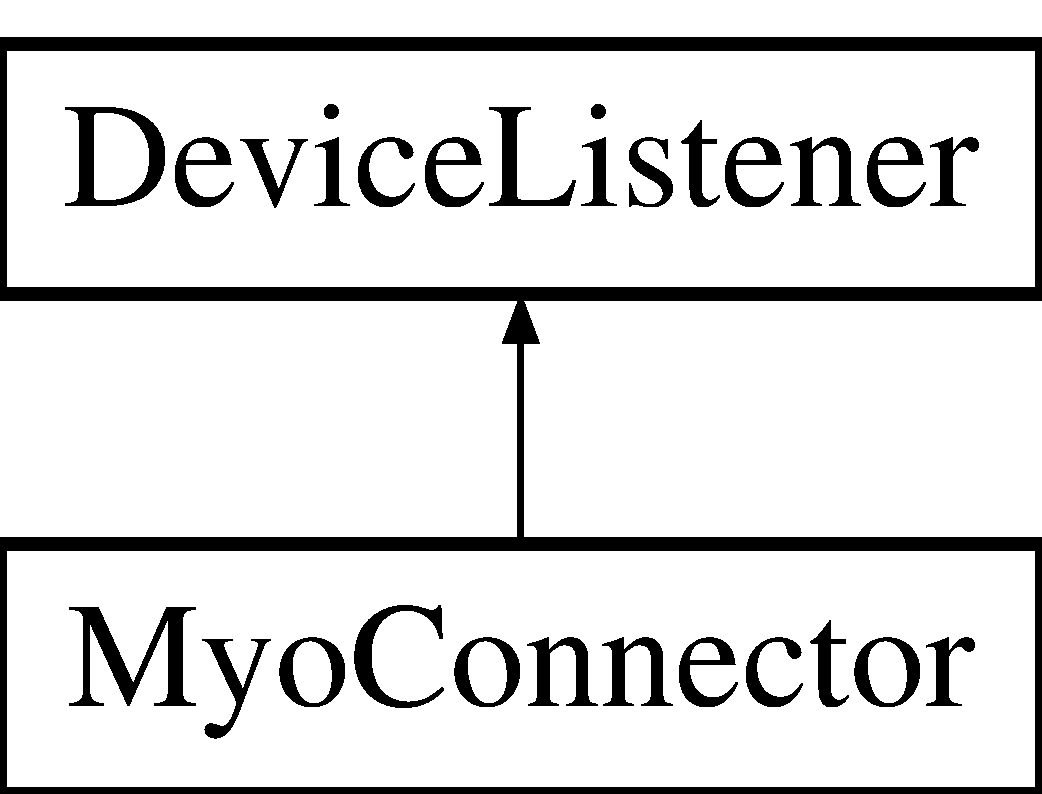
\includegraphics[height=2.000000cm]{classMyoConnector}
\end{center}
\end{figure}
\subsection*{Public Member Functions}
\begin{DoxyCompactItemize}
\item 
\hyperlink{classMyoConnector_a42308102b85259c441d806f94bd4caf1}{Myo\+Connector} ()
\item 
string \hyperlink{classMyoConnector_a3e5f18609811079ff25846d9b48c30b3}{get\+Current\+Pose} ()
\item 
vec3 \hyperlink{classMyoConnector_aa43b05a1bf5e27001464f2d70fcbf37e}{get\+Directions} ()
\item 
void \hyperlink{classMyoConnector_a9969e82f11eed7319a830f1cc9c7150c}{on\+Arm\+Sync} (Myo $\ast$myo, uint64\+\_\+t timestamp, Arm arm, X\+Direction x\+Direction, float rotation, Warmup\+State warmup\+State)
\item 
void \hyperlink{classMyoConnector_a3619d2595bc4e7585932aca0756d03dd}{on\+Arm\+Unsync} (Myo $\ast$myo, uint64\+\_\+t timestamp)
\item 
void \hyperlink{classMyoConnector_a64e4ea6befbf348461fe34998729da01}{on\+Lock} (Myo $\ast$myo, uint64\+\_\+t timestamp)
\item 
void \hyperlink{classMyoConnector_ae38c04a23931c6b8f789c28cdede6a08}{on\+Orientation\+Data} (Myo $\ast$myo, uint64\+\_\+t timestamp, const Quaternion$<$ float $>$ \&quat)
\item 
void \hyperlink{classMyoConnector_ab72e7aff6230ae3926c226172d1d5b7c}{on\+Pose} (Myo $\ast$myo, uint64\+\_\+t timestamp, Pose pose)
\item 
void \hyperlink{classMyoConnector_a35c2bda2592781885efdae984acfd92e}{on\+Unlock} (Myo $\ast$myo, uint64\+\_\+t timestamp)
\item 
void \hyperlink{classMyoConnector_a63c5e27ece98d6d24b2d8ff7ad230c1c}{on\+Unpair} (Myo $\ast$myo, uint64\+\_\+t timestamp)
\item 
void \hyperlink{classMyoConnector_a5c9a4a90f78daed7b7cac82cf4ea59f0}{print} ()
\end{DoxyCompactItemize}
\subsection*{Private Attributes}
\begin{DoxyCompactItemize}
\item 
Pose \hyperlink{classMyoConnector_a2146661def24d826ce3b42cef102be9b}{current\+Pose}
\item 
bool \hyperlink{classMyoConnector_a5df170788264f552feffe6a4eee54be8}{is\+Unlocked}
\item 
bool \hyperlink{classMyoConnector_a16bb4ab235d7e2c4b2d00554f8cda899}{on\+Arm}
\item 
int \hyperlink{classMyoConnector_a9005025e75f04acef5f587b2315b0f5c}{pitch\+\_\+w}
\item 
int \hyperlink{classMyoConnector_a373d10d0e950eeed40e9f31299c92dac}{roll\+\_\+w}
\item 
Arm \hyperlink{classMyoConnector_aa4054bb7438f07bf8109d54fc8be3f58}{which\+Arm}
\item 
int \hyperlink{classMyoConnector_a1ed4453c60238a7eca696500cb1d2c4e}{yaw\+\_\+w}
\end{DoxyCompactItemize}


\subsection{Detailed Description}
Classes that inherit from myo\+::\+Device\+Listener can be used to receive events from Myo devices. Device\+Listener provides several virtual functions for handling different kinds of events. If you do not override an event, the default behavior is to do nothing. 

\subsection{Constructor \& Destructor Documentation}
\index{Myo\+Connector@{Myo\+Connector}!Myo\+Connector@{Myo\+Connector}}
\index{Myo\+Connector@{Myo\+Connector}!Myo\+Connector@{Myo\+Connector}}
\subsubsection[{\texorpdfstring{Myo\+Connector()}{MyoConnector()}}]{\setlength{\rightskip}{0pt plus 5cm}Myo\+Connector\+::\+Myo\+Connector (
\begin{DoxyParamCaption}
{}
\end{DoxyParamCaption}
)}\hypertarget{classMyoConnector_a42308102b85259c441d806f94bd4caf1}{}\label{classMyoConnector_a42308102b85259c441d806f94bd4caf1}
It is used to generate an instance of the \hyperlink{classMyoConnector}{Myo\+Connector} class and link it to the already created Hub object. 

\subsection{Member Function Documentation}
\index{Myo\+Connector@{Myo\+Connector}!get\+Current\+Pose@{get\+Current\+Pose}}
\index{get\+Current\+Pose@{get\+Current\+Pose}!Myo\+Connector@{Myo\+Connector}}
\subsubsection[{\texorpdfstring{get\+Current\+Pose()}{getCurrentPose()}}]{\setlength{\rightskip}{0pt plus 5cm}string Myo\+Connector\+::get\+Current\+Pose (
\begin{DoxyParamCaption}
{}
\end{DoxyParamCaption}
)}\hypertarget{classMyoConnector_a3e5f18609811079ff25846d9b48c30b3}{}\label{classMyoConnector_a3e5f18609811079ff25846d9b48c30b3}
It returns the current pose, read by the on\+Pose function whenever the Myo detects that the person wearing it has changed their pose. \index{Myo\+Connector@{Myo\+Connector}!get\+Directions@{get\+Directions}}
\index{get\+Directions@{get\+Directions}!Myo\+Connector@{Myo\+Connector}}
\subsubsection[{\texorpdfstring{get\+Directions()}{getDirections()}}]{\setlength{\rightskip}{0pt plus 5cm}vec3 Myo\+Connector\+::get\+Directions (
\begin{DoxyParamCaption}
{}
\end{DoxyParamCaption}
)}\hypertarget{classMyoConnector_aa43b05a1bf5e27001464f2d70fcbf37e}{}\label{classMyoConnector_aa43b05a1bf5e27001464f2d70fcbf37e}
It returns the current pitch, roll and yaw values. \index{Myo\+Connector@{Myo\+Connector}!on\+Arm\+Sync@{on\+Arm\+Sync}}
\index{on\+Arm\+Sync@{on\+Arm\+Sync}!Myo\+Connector@{Myo\+Connector}}
\subsubsection[{\texorpdfstring{on\+Arm\+Sync(\+Myo $\ast$myo, uint64\+\_\+t timestamp, Arm arm, X\+Direction x\+Direction, float rotation, Warmup\+State warmup\+State)}{onArmSync(Myo *myo, uint64_t timestamp, Arm arm, XDirection xDirection, float rotation, WarmupState warmupState)}}]{\setlength{\rightskip}{0pt plus 5cm}void Myo\+Connector\+::on\+Arm\+Sync (
\begin{DoxyParamCaption}
\item[{Myo $\ast$}]{myo, }
\item[{uint64\+\_\+t}]{timestamp, }
\item[{Arm}]{arm, }
\item[{X\+Direction}]{x\+Direction, }
\item[{float}]{rotation, }
\item[{Warmup\+State}]{warmup\+State}
\end{DoxyParamCaption}
)}\hypertarget{classMyoConnector_a9969e82f11eed7319a830f1cc9c7150c}{}\label{classMyoConnector_a9969e82f11eed7319a830f1cc9c7150c}
Called when a paired Myo recognizes that it is on an arm. \index{Myo\+Connector@{Myo\+Connector}!on\+Arm\+Unsync@{on\+Arm\+Unsync}}
\index{on\+Arm\+Unsync@{on\+Arm\+Unsync}!Myo\+Connector@{Myo\+Connector}}
\subsubsection[{\texorpdfstring{on\+Arm\+Unsync(\+Myo $\ast$myo, uint64\+\_\+t timestamp)}{onArmUnsync(Myo *myo, uint64_t timestamp)}}]{\setlength{\rightskip}{0pt plus 5cm}void Myo\+Connector\+::on\+Arm\+Unsync (
\begin{DoxyParamCaption}
\item[{Myo $\ast$}]{myo, }
\item[{uint64\+\_\+t}]{timestamp}
\end{DoxyParamCaption}
)}\hypertarget{classMyoConnector_a3619d2595bc4e7585932aca0756d03dd}{}\label{classMyoConnector_a3619d2595bc4e7585932aca0756d03dd}
Called when a paired Myo is moved or removed from the arm. \index{Myo\+Connector@{Myo\+Connector}!on\+Lock@{on\+Lock}}
\index{on\+Lock@{on\+Lock}!Myo\+Connector@{Myo\+Connector}}
\subsubsection[{\texorpdfstring{on\+Lock(\+Myo $\ast$myo, uint64\+\_\+t timestamp)}{onLock(Myo *myo, uint64_t timestamp)}}]{\setlength{\rightskip}{0pt plus 5cm}void Myo\+Connector\+::on\+Lock (
\begin{DoxyParamCaption}
\item[{Myo $\ast$}]{myo, }
\item[{uint64\+\_\+t}]{timestamp}
\end{DoxyParamCaption}
)}\hypertarget{classMyoConnector_a64e4ea6befbf348461fe34998729da01}{}\label{classMyoConnector_a64e4ea6befbf348461fe34998729da01}
Called when a paired Myo becomes locked. \index{Myo\+Connector@{Myo\+Connector}!on\+Orientation\+Data@{on\+Orientation\+Data}}
\index{on\+Orientation\+Data@{on\+Orientation\+Data}!Myo\+Connector@{Myo\+Connector}}
\subsubsection[{\texorpdfstring{on\+Orientation\+Data(\+Myo $\ast$myo, uint64\+\_\+t timestamp, const Quaternion$<$ float $>$ \&quat)}{onOrientationData(Myo *myo, uint64_t timestamp, const Quaternion< float > &quat)}}]{\setlength{\rightskip}{0pt plus 5cm}void Myo\+Connector\+::on\+Orientation\+Data (
\begin{DoxyParamCaption}
\item[{Myo $\ast$}]{myo, }
\item[{uint64\+\_\+t}]{timestamp, }
\item[{const Quaternion$<$ float $>$ \&}]{quat}
\end{DoxyParamCaption}
)}\hypertarget{classMyoConnector_ae38c04a23931c6b8f789c28cdede6a08}{}\label{classMyoConnector_ae38c04a23931c6b8f789c28cdede6a08}
Called when a paired Myo has provided new orientation data. \index{Myo\+Connector@{Myo\+Connector}!on\+Pose@{on\+Pose}}
\index{on\+Pose@{on\+Pose}!Myo\+Connector@{Myo\+Connector}}
\subsubsection[{\texorpdfstring{on\+Pose(\+Myo $\ast$myo, uint64\+\_\+t timestamp, Pose pose)}{onPose(Myo *myo, uint64_t timestamp, Pose pose)}}]{\setlength{\rightskip}{0pt plus 5cm}void Myo\+Connector\+::on\+Pose (
\begin{DoxyParamCaption}
\item[{Myo $\ast$}]{myo, }
\item[{uint64\+\_\+t}]{timestamp, }
\item[{Pose}]{pose}
\end{DoxyParamCaption}
)}\hypertarget{classMyoConnector_ab72e7aff6230ae3926c226172d1d5b7c}{}\label{classMyoConnector_ab72e7aff6230ae3926c226172d1d5b7c}
Called when a paired Myo has provided a new pose. \index{Myo\+Connector@{Myo\+Connector}!on\+Unlock@{on\+Unlock}}
\index{on\+Unlock@{on\+Unlock}!Myo\+Connector@{Myo\+Connector}}
\subsubsection[{\texorpdfstring{on\+Unlock(\+Myo $\ast$myo, uint64\+\_\+t timestamp)}{onUnlock(Myo *myo, uint64_t timestamp)}}]{\setlength{\rightskip}{0pt plus 5cm}void Myo\+Connector\+::on\+Unlock (
\begin{DoxyParamCaption}
\item[{Myo $\ast$}]{myo, }
\item[{uint64\+\_\+t}]{timestamp}
\end{DoxyParamCaption}
)}\hypertarget{classMyoConnector_a35c2bda2592781885efdae984acfd92e}{}\label{classMyoConnector_a35c2bda2592781885efdae984acfd92e}
Called when a paired Myo becomes unlocked. \index{Myo\+Connector@{Myo\+Connector}!on\+Unpair@{on\+Unpair}}
\index{on\+Unpair@{on\+Unpair}!Myo\+Connector@{Myo\+Connector}}
\subsubsection[{\texorpdfstring{on\+Unpair(\+Myo $\ast$myo, uint64\+\_\+t timestamp)}{onUnpair(Myo *myo, uint64_t timestamp)}}]{\setlength{\rightskip}{0pt plus 5cm}void Myo\+Connector\+::on\+Unpair (
\begin{DoxyParamCaption}
\item[{Myo $\ast$}]{myo, }
\item[{uint64\+\_\+t}]{timestamp}
\end{DoxyParamCaption}
)}\hypertarget{classMyoConnector_a63c5e27ece98d6d24b2d8ff7ad230c1c}{}\label{classMyoConnector_a63c5e27ece98d6d24b2d8ff7ad230c1c}
Called when a Myo has been unpaired. \index{Myo\+Connector@{Myo\+Connector}!print@{print}}
\index{print@{print}!Myo\+Connector@{Myo\+Connector}}
\subsubsection[{\texorpdfstring{print()}{print()}}]{\setlength{\rightskip}{0pt plus 5cm}void Myo\+Connector\+::print (
\begin{DoxyParamCaption}
{}
\end{DoxyParamCaption}
)}\hypertarget{classMyoConnector_a5c9a4a90f78daed7b7cac82cf4ea59f0}{}\label{classMyoConnector_a5c9a4a90f78daed7b7cac82cf4ea59f0}
It prints the current values that were updated by the overriden virtual functions. 

\subsection{Field Documentation}
\index{Myo\+Connector@{Myo\+Connector}!current\+Pose@{current\+Pose}}
\index{current\+Pose@{current\+Pose}!Myo\+Connector@{Myo\+Connector}}
\subsubsection[{\texorpdfstring{current\+Pose}{currentPose}}]{\setlength{\rightskip}{0pt plus 5cm}Pose Myo\+Connector\+::current\+Pose\hspace{0.3cm}{\ttfamily [private]}}\hypertarget{classMyoConnector_a2146661def24d826ce3b42cef102be9b}{}\label{classMyoConnector_a2146661def24d826ce3b42cef102be9b}
It stores the value returned by the on\+Pose funtion, which represents the pose detected in the current frame. \index{Myo\+Connector@{Myo\+Connector}!is\+Unlocked@{is\+Unlocked}}
\index{is\+Unlocked@{is\+Unlocked}!Myo\+Connector@{Myo\+Connector}}
\subsubsection[{\texorpdfstring{is\+Unlocked}{isUnlocked}}]{\setlength{\rightskip}{0pt plus 5cm}bool Myo\+Connector\+::is\+Unlocked\hspace{0.3cm}{\ttfamily [private]}}\hypertarget{classMyoConnector_a5df170788264f552feffe6a4eee54be8}{}\label{classMyoConnector_a5df170788264f552feffe6a4eee54be8}
It stores the value returned by the on\+Lock and on\+Unlock funtions, which represents wheter or not the user has unlocked the paired Myo armband. \index{Myo\+Connector@{Myo\+Connector}!on\+Arm@{on\+Arm}}
\index{on\+Arm@{on\+Arm}!Myo\+Connector@{Myo\+Connector}}
\subsubsection[{\texorpdfstring{on\+Arm}{onArm}}]{\setlength{\rightskip}{0pt plus 5cm}bool Myo\+Connector\+::on\+Arm\hspace{0.3cm}{\ttfamily [private]}}\hypertarget{classMyoConnector_a16bb4ab235d7e2c4b2d00554f8cda899}{}\label{classMyoConnector_a16bb4ab235d7e2c4b2d00554f8cda899}
It stores the value returned by the on\+Arm\+Sync and on\+Arm\+Unsync funtions, which represents wheter or not the user is wearing the paired Myo armband. \index{Myo\+Connector@{Myo\+Connector}!pitch\+\_\+w@{pitch\+\_\+w}}
\index{pitch\+\_\+w@{pitch\+\_\+w}!Myo\+Connector@{Myo\+Connector}}
\subsubsection[{\texorpdfstring{pitch\+\_\+w}{pitch_w}}]{\setlength{\rightskip}{0pt plus 5cm}int Myo\+Connector\+::pitch\+\_\+w\hspace{0.3cm}{\ttfamily [private]}}\hypertarget{classMyoConnector_a9005025e75f04acef5f587b2315b0f5c}{}\label{classMyoConnector_a9005025e75f04acef5f587b2315b0f5c}
It stores the value returned by the on\+Orientation\+Data funtion, which represents the pitch Euler angle, obtained from the unit quaternion. \index{Myo\+Connector@{Myo\+Connector}!roll\+\_\+w@{roll\+\_\+w}}
\index{roll\+\_\+w@{roll\+\_\+w}!Myo\+Connector@{Myo\+Connector}}
\subsubsection[{\texorpdfstring{roll\+\_\+w}{roll_w}}]{\setlength{\rightskip}{0pt plus 5cm}int Myo\+Connector\+::roll\+\_\+w\hspace{0.3cm}{\ttfamily [private]}}\hypertarget{classMyoConnector_a373d10d0e950eeed40e9f31299c92dac}{}\label{classMyoConnector_a373d10d0e950eeed40e9f31299c92dac}
It stores the value returned by the on\+Orientation\+Data funtion, which represents the roll Euler angle, obtained from the unit quaternion. \index{Myo\+Connector@{Myo\+Connector}!which\+Arm@{which\+Arm}}
\index{which\+Arm@{which\+Arm}!Myo\+Connector@{Myo\+Connector}}
\subsubsection[{\texorpdfstring{which\+Arm}{whichArm}}]{\setlength{\rightskip}{0pt plus 5cm}Arm Myo\+Connector\+::which\+Arm\hspace{0.3cm}{\ttfamily [private]}}\hypertarget{classMyoConnector_aa4054bb7438f07bf8109d54fc8be3f58}{}\label{classMyoConnector_aa4054bb7438f07bf8109d54fc8be3f58}
It stores the value returned by the on\+Arm\+Sync and on\+Arm\+Unsync funtions, which represents on which arm the user is wearing the paired Myo armband. \index{Myo\+Connector@{Myo\+Connector}!yaw\+\_\+w@{yaw\+\_\+w}}
\index{yaw\+\_\+w@{yaw\+\_\+w}!Myo\+Connector@{Myo\+Connector}}
\subsubsection[{\texorpdfstring{yaw\+\_\+w}{yaw_w}}]{\setlength{\rightskip}{0pt plus 5cm}int Myo\+Connector\+::yaw\+\_\+w\hspace{0.3cm}{\ttfamily [private]}}\hypertarget{classMyoConnector_a1ed4453c60238a7eca696500cb1d2c4e}{}\label{classMyoConnector_a1ed4453c60238a7eca696500cb1d2c4e}
It stores the value returned by the on\+Orientation\+Data funtion, which represents the yaw Euler angle, obtained from the unit quaternion. 

The documentation for this class was generated from the following file\+:\begin{DoxyCompactItemize}
\item 
\hyperlink{MyoConnector_8h}{Myo\+Connector.\+h}\end{DoxyCompactItemize}

\hypertarget{classSettings}{}\section{Settings Class Reference}
\label{classSettings}\index{Settings@{Settings}}


{\ttfamily \#include $<$Settings.\+h$>$}

\subsection*{Public Member Functions}
\begin{DoxyCompactItemize}
\item 
\hyperlink{classSettings_ab7169a6eefce79566dd07db3b1e5e967}{Settings} ()
\item 
bool \hyperlink{classSettings_ac9ecd28f72588f8481840c83de4f9905}{get\+Down\+Animation} ()
\item 
bool \hyperlink{classSettings_ab111ded63b457ef62ba4d3c2b5fd505f}{get\+Fade\+Left\+Animation} ()
\item 
bool \hyperlink{classSettings_aac9a6dcb72f803ed1a8c60815a57d120}{get\+Fade\+Right\+Animation} ()
\item 
vector$<$ Drawable $\ast$ $>$ \hyperlink{classSettings_a3f4a91c18915f999622a98b88d815007}{get\+Objects\+Vector} ()
\item 
bool \hyperlink{classSettings_ac66a0a23351662d86679addd4b058e1a}{get\+Scroll\+Down\+Animation} ()
\item 
bool \hyperlink{classSettings_a6681474ab3a4d082a1ccafb0015393db}{get\+Scroll\+Up\+Animation} ()
\item 
bool \hyperlink{classSettings_a01ae940ebfaa263e7178d38740bdd332}{get\+Up\+Animation} ()
\item 
void \hyperlink{classSettings_a38d541933e0786f211e6296b03d9f002}{set\+Down\+Animation} (bool \hyperlink{classSettings_a3ca98c2832652c799e4156c2cd9870b8}{down\+Animation})
\item 
void \hyperlink{classSettings_abd4b4ba65f26dc0f542c74dd977404a6}{set\+Fade\+Left\+Animation} (bool \hyperlink{classSettings_a9fc3029b2d7ea3627cfb337963e5e517}{fade\+Left\+Animation})
\item 
void \hyperlink{classSettings_aef8cac960c79056f81bcc62d58332555}{set\+Fade\+Right\+Animation} (bool \hyperlink{classSettings_a361d40b16e3a783d7ac48008a825da86}{fade\+Right\+Animation})
\item 
void \hyperlink{classSettings_a4b512ec5f1d7a5440c5aa81ebb93dd63}{set\+Scroll\+Down\+Animation} (bool \hyperlink{classSettings_ae02e88347857994296383bea194f3fdf}{scroll\+Down\+Animation})
\item 
void \hyperlink{classSettings_a3527753c47290e4a3de380cc62abe353}{set\+Scroll\+Up\+Animation} (bool \hyperlink{classSettings_acef41c3ecdc8d54ae52e9dacf6a47bec}{scroll\+Up\+Animation})
\item 
void \hyperlink{classSettings_a3976a636038110c89e23506cfd980707}{settings\+Events} ()
\item 
void \hyperlink{classSettings_a176dc32eec32d3e22a2cb49a59f4f279}{set\+Up\+Animation} (bool \hyperlink{classSettings_a67a1520a803f8cd6c45d236f0be4796f}{up\+Animation})
\item 
void \hyperlink{classSettings_a042d54c37551fb94fc180557bb0b845f}{test} ()
\end{DoxyCompactItemize}
\subsection*{Private Member Functions}
\begin{DoxyCompactItemize}
\item 
void \hyperlink{classSettings_a57496310fa30eb01c0cf2d5c5a0b1119}{animate\+Down} ()
\item 
void \hyperlink{classSettings_aaf7aa8eba2a6e9cf3c69d417bfac45e3}{animate\+Up} ()
\item 
void \hyperlink{classSettings_aadfdd9d712f92c22f3bf7ea219df51fb}{fade\+Left} ()
\item 
void \hyperlink{classSettings_aea96eb70c9a38159ae38f514e6f598d2}{fade\+Right} ()
\item 
void \hyperlink{classSettings_ad47a8d3f696dcb0d38c1dc5088008885}{init} ()
\item 
void \hyperlink{classSettings_a5990c74e2a9622a466a69a45052eabed}{page\+Down} ()
\item 
void \hyperlink{classSettings_abd533093c1ebef5545eba511e95c5d65}{page\+Up} ()
\item 
void \hyperlink{classSettings_a455628093679d8ff5661f0cf17c45ea9}{scroll\+Down} ()
\item 
void \hyperlink{classSettings_aae74a0b5718c3a2c47725e12e96f634a}{scroll\+Up} ()
\end{DoxyCompactItemize}
\subsection*{Private Attributes}
\begin{DoxyCompactItemize}
\item 
float \hyperlink{classSettings_ad4ed30795fceb42b02937d87bac50213}{alpha}
\item 
float \hyperlink{classSettings_ae0dc78ef4c9a43cfd7d0a1b7fc2c1576}{animation\+Speed}
\item 
float \hyperlink{classSettings_ac8d966b3fddad984eb3448c82da52766}{animation\+Time}
\item 
Rectangle\+Shape \hyperlink{classSettings_adfb55e6a4950331071235bdf71e70635}{background}
\item 
bool \hyperlink{classSettings_a3ca98c2832652c799e4156c2cd9870b8}{down\+Animation}
\item 
bool \hyperlink{classSettings_a9fc3029b2d7ea3627cfb337963e5e517}{fade\+Left\+Animation}
\item 
bool \hyperlink{classSettings_a361d40b16e3a783d7ac48008a825da86}{fade\+Right\+Animation}
\item 
float \hyperlink{classSettings_ae8d4f4e2e7ff6fe49ae1fde8d5d60e3d}{fade\+Speed}
\item 
float \hyperlink{classSettings_af99154745965d7887d876893cb728d68}{fade\+Time}
\item 
int \hyperlink{classSettings_ac3d8cbf9380fd8b725e8ebd1b37b5ee6}{n\+Settings}
\item 
vector$<$ int $>$ \hyperlink{classSettings_ae35f4a510650ec63a9ef68c983b5c5f2}{options\+Positions}
\item 
vector$<$ vector$<$ Text $>$ $>$ \hyperlink{classSettings_a112aa156eec22f1984ff6f98afcec7bb}{options\+Texts}
\item 
bool \hyperlink{classSettings_a503fc01d9f2c446eb665f73f4b0bdb84}{page\+Down\+Animation}
\item 
int \hyperlink{classSettings_a57913d133488d8cd62688bfcc483b0a4}{page\+Header\+Position}
\item 
bool \hyperlink{classSettings_a382d15210e0204c9fe59a54577b25eee}{page\+Up\+Animation}
\item 
bool \hyperlink{classSettings_ae02e88347857994296383bea194f3fdf}{scroll\+Down\+Animation}
\item 
bool \hyperlink{classSettings_acef41c3ecdc8d54ae52e9dacf6a47bec}{scroll\+Up\+Animation}
\item 
bool \hyperlink{classSettings_af2fdd4e36866cd1e773749e4d3c8e36b}{second\+Fade}
\item 
Rectangle\+Shape \hyperlink{classSettings_ad13324ea78b1a08300d96d84a7a37428}{selector}
\item 
int \hyperlink{classSettings_a7c479137ff0b1327f7ba30f5d0d07536}{selector\+Position}
\item 
Font \hyperlink{classSettings_a92b2a2888b774616737fa42418049bd1}{settings\+Font}
\item 
vector$<$ Text $>$ \hyperlink{classSettings_a7bbaff0d17c72a260f549c66d216d6dd}{settings\+Texts}
\item 
int \hyperlink{classSettings_a28d934a64de46650bfb0d238dbd6ee60}{step\+Counter}
\item 
float \hyperlink{classSettings_ae5a8d76a1a6cdd6d75944bbbdde48d43}{text\+Margin}
\item 
unsigned int \hyperlink{classSettings_abea7382c4fbb098421588012e1d1461b}{text\+Size}
\item 
float \hyperlink{classSettings_a16af6d82edc8cea82f4c5642fd9d2245}{thickness}
\item 
vector$<$ Drawable $\ast$ $>$ \hyperlink{classSettings_a53bcf11bcc5148c0bfd512deb7d45fb3}{to\+Draw}
\item 
float \hyperlink{classSettings_a3fbbf163b14eb206150c9fd83b054562}{ud\+Animation\+Speed}
\item 
bool \hyperlink{classSettings_a67a1520a803f8cd6c45d236f0be4796f}{up\+Animation}
\end{DoxyCompactItemize}


\subsection{Constructor \& Destructor Documentation}
\index{Settings@{Settings}!Settings@{Settings}}
\index{Settings@{Settings}!Settings@{Settings}}
\subsubsection[{\texorpdfstring{Settings()}{Settings()}}]{\setlength{\rightskip}{0pt plus 5cm}Settings\+::\+Settings (
\begin{DoxyParamCaption}
{}
\end{DoxyParamCaption}
)}\hypertarget{classSettings_ab7169a6eefce79566dd07db3b1e5e967}{}\label{classSettings_ab7169a6eefce79566dd07db3b1e5e967}


\subsection{Member Function Documentation}
\index{Settings@{Settings}!animate\+Down@{animate\+Down}}
\index{animate\+Down@{animate\+Down}!Settings@{Settings}}
\subsubsection[{\texorpdfstring{animate\+Down()}{animateDown()}}]{\setlength{\rightskip}{0pt plus 5cm}void Settings\+::animate\+Down (
\begin{DoxyParamCaption}
{}
\end{DoxyParamCaption}
)\hspace{0.3cm}{\ttfamily [private]}}\hypertarget{classSettings_a57496310fa30eb01c0cf2d5c5a0b1119}{}\label{classSettings_a57496310fa30eb01c0cf2d5c5a0b1119}
\index{Settings@{Settings}!animate\+Up@{animate\+Up}}
\index{animate\+Up@{animate\+Up}!Settings@{Settings}}
\subsubsection[{\texorpdfstring{animate\+Up()}{animateUp()}}]{\setlength{\rightskip}{0pt plus 5cm}void Settings\+::animate\+Up (
\begin{DoxyParamCaption}
{}
\end{DoxyParamCaption}
)\hspace{0.3cm}{\ttfamily [private]}}\hypertarget{classSettings_aaf7aa8eba2a6e9cf3c69d417bfac45e3}{}\label{classSettings_aaf7aa8eba2a6e9cf3c69d417bfac45e3}
\index{Settings@{Settings}!fade\+Left@{fade\+Left}}
\index{fade\+Left@{fade\+Left}!Settings@{Settings}}
\subsubsection[{\texorpdfstring{fade\+Left()}{fadeLeft()}}]{\setlength{\rightskip}{0pt plus 5cm}void Settings\+::fade\+Left (
\begin{DoxyParamCaption}
{}
\end{DoxyParamCaption}
)\hspace{0.3cm}{\ttfamily [private]}}\hypertarget{classSettings_aadfdd9d712f92c22f3bf7ea219df51fb}{}\label{classSettings_aadfdd9d712f92c22f3bf7ea219df51fb}
\index{Settings@{Settings}!fade\+Right@{fade\+Right}}
\index{fade\+Right@{fade\+Right}!Settings@{Settings}}
\subsubsection[{\texorpdfstring{fade\+Right()}{fadeRight()}}]{\setlength{\rightskip}{0pt plus 5cm}void Settings\+::fade\+Right (
\begin{DoxyParamCaption}
{}
\end{DoxyParamCaption}
)\hspace{0.3cm}{\ttfamily [private]}}\hypertarget{classSettings_aea96eb70c9a38159ae38f514e6f598d2}{}\label{classSettings_aea96eb70c9a38159ae38f514e6f598d2}
\index{Settings@{Settings}!get\+Down\+Animation@{get\+Down\+Animation}}
\index{get\+Down\+Animation@{get\+Down\+Animation}!Settings@{Settings}}
\subsubsection[{\texorpdfstring{get\+Down\+Animation()}{getDownAnimation()}}]{\setlength{\rightskip}{0pt plus 5cm}bool Settings\+::get\+Down\+Animation (
\begin{DoxyParamCaption}
{}
\end{DoxyParamCaption}
)}\hypertarget{classSettings_ac9ecd28f72588f8481840c83de4f9905}{}\label{classSettings_ac9ecd28f72588f8481840c83de4f9905}
\index{Settings@{Settings}!get\+Fade\+Left\+Animation@{get\+Fade\+Left\+Animation}}
\index{get\+Fade\+Left\+Animation@{get\+Fade\+Left\+Animation}!Settings@{Settings}}
\subsubsection[{\texorpdfstring{get\+Fade\+Left\+Animation()}{getFadeLeftAnimation()}}]{\setlength{\rightskip}{0pt plus 5cm}bool Settings\+::get\+Fade\+Left\+Animation (
\begin{DoxyParamCaption}
{}
\end{DoxyParamCaption}
)}\hypertarget{classSettings_ab111ded63b457ef62ba4d3c2b5fd505f}{}\label{classSettings_ab111ded63b457ef62ba4d3c2b5fd505f}
\index{Settings@{Settings}!get\+Fade\+Right\+Animation@{get\+Fade\+Right\+Animation}}
\index{get\+Fade\+Right\+Animation@{get\+Fade\+Right\+Animation}!Settings@{Settings}}
\subsubsection[{\texorpdfstring{get\+Fade\+Right\+Animation()}{getFadeRightAnimation()}}]{\setlength{\rightskip}{0pt plus 5cm}bool Settings\+::get\+Fade\+Right\+Animation (
\begin{DoxyParamCaption}
{}
\end{DoxyParamCaption}
)}\hypertarget{classSettings_aac9a6dcb72f803ed1a8c60815a57d120}{}\label{classSettings_aac9a6dcb72f803ed1a8c60815a57d120}
\index{Settings@{Settings}!get\+Objects\+Vector@{get\+Objects\+Vector}}
\index{get\+Objects\+Vector@{get\+Objects\+Vector}!Settings@{Settings}}
\subsubsection[{\texorpdfstring{get\+Objects\+Vector()}{getObjectsVector()}}]{\setlength{\rightskip}{0pt plus 5cm}vector$<$Drawable$\ast$$>$ Settings\+::get\+Objects\+Vector (
\begin{DoxyParamCaption}
{}
\end{DoxyParamCaption}
)}\hypertarget{classSettings_a3f4a91c18915f999622a98b88d815007}{}\label{classSettings_a3f4a91c18915f999622a98b88d815007}
\index{Settings@{Settings}!get\+Scroll\+Down\+Animation@{get\+Scroll\+Down\+Animation}}
\index{get\+Scroll\+Down\+Animation@{get\+Scroll\+Down\+Animation}!Settings@{Settings}}
\subsubsection[{\texorpdfstring{get\+Scroll\+Down\+Animation()}{getScrollDownAnimation()}}]{\setlength{\rightskip}{0pt plus 5cm}bool Settings\+::get\+Scroll\+Down\+Animation (
\begin{DoxyParamCaption}
{}
\end{DoxyParamCaption}
)}\hypertarget{classSettings_ac66a0a23351662d86679addd4b058e1a}{}\label{classSettings_ac66a0a23351662d86679addd4b058e1a}
\index{Settings@{Settings}!get\+Scroll\+Up\+Animation@{get\+Scroll\+Up\+Animation}}
\index{get\+Scroll\+Up\+Animation@{get\+Scroll\+Up\+Animation}!Settings@{Settings}}
\subsubsection[{\texorpdfstring{get\+Scroll\+Up\+Animation()}{getScrollUpAnimation()}}]{\setlength{\rightskip}{0pt plus 5cm}bool Settings\+::get\+Scroll\+Up\+Animation (
\begin{DoxyParamCaption}
{}
\end{DoxyParamCaption}
)}\hypertarget{classSettings_a6681474ab3a4d082a1ccafb0015393db}{}\label{classSettings_a6681474ab3a4d082a1ccafb0015393db}
\index{Settings@{Settings}!get\+Up\+Animation@{get\+Up\+Animation}}
\index{get\+Up\+Animation@{get\+Up\+Animation}!Settings@{Settings}}
\subsubsection[{\texorpdfstring{get\+Up\+Animation()}{getUpAnimation()}}]{\setlength{\rightskip}{0pt plus 5cm}bool Settings\+::get\+Up\+Animation (
\begin{DoxyParamCaption}
{}
\end{DoxyParamCaption}
)}\hypertarget{classSettings_a01ae940ebfaa263e7178d38740bdd332}{}\label{classSettings_a01ae940ebfaa263e7178d38740bdd332}
\index{Settings@{Settings}!init@{init}}
\index{init@{init}!Settings@{Settings}}
\subsubsection[{\texorpdfstring{init()}{init()}}]{\setlength{\rightskip}{0pt plus 5cm}void Settings\+::init (
\begin{DoxyParamCaption}
{}
\end{DoxyParamCaption}
)\hspace{0.3cm}{\ttfamily [private]}}\hypertarget{classSettings_ad47a8d3f696dcb0d38c1dc5088008885}{}\label{classSettings_ad47a8d3f696dcb0d38c1dc5088008885}
\index{Settings@{Settings}!page\+Down@{page\+Down}}
\index{page\+Down@{page\+Down}!Settings@{Settings}}
\subsubsection[{\texorpdfstring{page\+Down()}{pageDown()}}]{\setlength{\rightskip}{0pt plus 5cm}void Settings\+::page\+Down (
\begin{DoxyParamCaption}
{}
\end{DoxyParamCaption}
)\hspace{0.3cm}{\ttfamily [private]}}\hypertarget{classSettings_a5990c74e2a9622a466a69a45052eabed}{}\label{classSettings_a5990c74e2a9622a466a69a45052eabed}
\index{Settings@{Settings}!page\+Up@{page\+Up}}
\index{page\+Up@{page\+Up}!Settings@{Settings}}
\subsubsection[{\texorpdfstring{page\+Up()}{pageUp()}}]{\setlength{\rightskip}{0pt plus 5cm}void Settings\+::page\+Up (
\begin{DoxyParamCaption}
{}
\end{DoxyParamCaption}
)\hspace{0.3cm}{\ttfamily [private]}}\hypertarget{classSettings_abd533093c1ebef5545eba511e95c5d65}{}\label{classSettings_abd533093c1ebef5545eba511e95c5d65}
\index{Settings@{Settings}!scroll\+Down@{scroll\+Down}}
\index{scroll\+Down@{scroll\+Down}!Settings@{Settings}}
\subsubsection[{\texorpdfstring{scroll\+Down()}{scrollDown()}}]{\setlength{\rightskip}{0pt plus 5cm}void Settings\+::scroll\+Down (
\begin{DoxyParamCaption}
{}
\end{DoxyParamCaption}
)\hspace{0.3cm}{\ttfamily [private]}}\hypertarget{classSettings_a455628093679d8ff5661f0cf17c45ea9}{}\label{classSettings_a455628093679d8ff5661f0cf17c45ea9}
\index{Settings@{Settings}!scroll\+Up@{scroll\+Up}}
\index{scroll\+Up@{scroll\+Up}!Settings@{Settings}}
\subsubsection[{\texorpdfstring{scroll\+Up()}{scrollUp()}}]{\setlength{\rightskip}{0pt plus 5cm}void Settings\+::scroll\+Up (
\begin{DoxyParamCaption}
{}
\end{DoxyParamCaption}
)\hspace{0.3cm}{\ttfamily [private]}}\hypertarget{classSettings_aae74a0b5718c3a2c47725e12e96f634a}{}\label{classSettings_aae74a0b5718c3a2c47725e12e96f634a}
\index{Settings@{Settings}!set\+Down\+Animation@{set\+Down\+Animation}}
\index{set\+Down\+Animation@{set\+Down\+Animation}!Settings@{Settings}}
\subsubsection[{\texorpdfstring{set\+Down\+Animation(bool down\+Animation)}{setDownAnimation(bool downAnimation)}}]{\setlength{\rightskip}{0pt plus 5cm}void Settings\+::set\+Down\+Animation (
\begin{DoxyParamCaption}
\item[{bool}]{down\+Animation}
\end{DoxyParamCaption}
)}\hypertarget{classSettings_a38d541933e0786f211e6296b03d9f002}{}\label{classSettings_a38d541933e0786f211e6296b03d9f002}
\index{Settings@{Settings}!set\+Fade\+Left\+Animation@{set\+Fade\+Left\+Animation}}
\index{set\+Fade\+Left\+Animation@{set\+Fade\+Left\+Animation}!Settings@{Settings}}
\subsubsection[{\texorpdfstring{set\+Fade\+Left\+Animation(bool fade\+Left\+Animation)}{setFadeLeftAnimation(bool fadeLeftAnimation)}}]{\setlength{\rightskip}{0pt plus 5cm}void Settings\+::set\+Fade\+Left\+Animation (
\begin{DoxyParamCaption}
\item[{bool}]{fade\+Left\+Animation}
\end{DoxyParamCaption}
)}\hypertarget{classSettings_abd4b4ba65f26dc0f542c74dd977404a6}{}\label{classSettings_abd4b4ba65f26dc0f542c74dd977404a6}
\index{Settings@{Settings}!set\+Fade\+Right\+Animation@{set\+Fade\+Right\+Animation}}
\index{set\+Fade\+Right\+Animation@{set\+Fade\+Right\+Animation}!Settings@{Settings}}
\subsubsection[{\texorpdfstring{set\+Fade\+Right\+Animation(bool fade\+Right\+Animation)}{setFadeRightAnimation(bool fadeRightAnimation)}}]{\setlength{\rightskip}{0pt plus 5cm}void Settings\+::set\+Fade\+Right\+Animation (
\begin{DoxyParamCaption}
\item[{bool}]{fade\+Right\+Animation}
\end{DoxyParamCaption}
)}\hypertarget{classSettings_aef8cac960c79056f81bcc62d58332555}{}\label{classSettings_aef8cac960c79056f81bcc62d58332555}
\index{Settings@{Settings}!set\+Scroll\+Down\+Animation@{set\+Scroll\+Down\+Animation}}
\index{set\+Scroll\+Down\+Animation@{set\+Scroll\+Down\+Animation}!Settings@{Settings}}
\subsubsection[{\texorpdfstring{set\+Scroll\+Down\+Animation(bool scroll\+Down\+Animation)}{setScrollDownAnimation(bool scrollDownAnimation)}}]{\setlength{\rightskip}{0pt plus 5cm}void Settings\+::set\+Scroll\+Down\+Animation (
\begin{DoxyParamCaption}
\item[{bool}]{scroll\+Down\+Animation}
\end{DoxyParamCaption}
)}\hypertarget{classSettings_a4b512ec5f1d7a5440c5aa81ebb93dd63}{}\label{classSettings_a4b512ec5f1d7a5440c5aa81ebb93dd63}
\index{Settings@{Settings}!set\+Scroll\+Up\+Animation@{set\+Scroll\+Up\+Animation}}
\index{set\+Scroll\+Up\+Animation@{set\+Scroll\+Up\+Animation}!Settings@{Settings}}
\subsubsection[{\texorpdfstring{set\+Scroll\+Up\+Animation(bool scroll\+Up\+Animation)}{setScrollUpAnimation(bool scrollUpAnimation)}}]{\setlength{\rightskip}{0pt plus 5cm}void Settings\+::set\+Scroll\+Up\+Animation (
\begin{DoxyParamCaption}
\item[{bool}]{scroll\+Up\+Animation}
\end{DoxyParamCaption}
)}\hypertarget{classSettings_a3527753c47290e4a3de380cc62abe353}{}\label{classSettings_a3527753c47290e4a3de380cc62abe353}
\index{Settings@{Settings}!settings\+Events@{settings\+Events}}
\index{settings\+Events@{settings\+Events}!Settings@{Settings}}
\subsubsection[{\texorpdfstring{settings\+Events()}{settingsEvents()}}]{\setlength{\rightskip}{0pt plus 5cm}void Settings\+::settings\+Events (
\begin{DoxyParamCaption}
{}
\end{DoxyParamCaption}
)}\hypertarget{classSettings_a3976a636038110c89e23506cfd980707}{}\label{classSettings_a3976a636038110c89e23506cfd980707}
\index{Settings@{Settings}!set\+Up\+Animation@{set\+Up\+Animation}}
\index{set\+Up\+Animation@{set\+Up\+Animation}!Settings@{Settings}}
\subsubsection[{\texorpdfstring{set\+Up\+Animation(bool up\+Animation)}{setUpAnimation(bool upAnimation)}}]{\setlength{\rightskip}{0pt plus 5cm}void Settings\+::set\+Up\+Animation (
\begin{DoxyParamCaption}
\item[{bool}]{up\+Animation}
\end{DoxyParamCaption}
)}\hypertarget{classSettings_a176dc32eec32d3e22a2cb49a59f4f279}{}\label{classSettings_a176dc32eec32d3e22a2cb49a59f4f279}
\index{Settings@{Settings}!test@{test}}
\index{test@{test}!Settings@{Settings}}
\subsubsection[{\texorpdfstring{test()}{test()}}]{\setlength{\rightskip}{0pt plus 5cm}void Settings\+::test (
\begin{DoxyParamCaption}
{}
\end{DoxyParamCaption}
)}\hypertarget{classSettings_a042d54c37551fb94fc180557bb0b845f}{}\label{classSettings_a042d54c37551fb94fc180557bb0b845f}


\subsection{Field Documentation}
\index{Settings@{Settings}!alpha@{alpha}}
\index{alpha@{alpha}!Settings@{Settings}}
\subsubsection[{\texorpdfstring{alpha}{alpha}}]{\setlength{\rightskip}{0pt plus 5cm}float Settings\+::alpha\hspace{0.3cm}{\ttfamily [private]}}\hypertarget{classSettings_ad4ed30795fceb42b02937d87bac50213}{}\label{classSettings_ad4ed30795fceb42b02937d87bac50213}
\index{Settings@{Settings}!animation\+Speed@{animation\+Speed}}
\index{animation\+Speed@{animation\+Speed}!Settings@{Settings}}
\subsubsection[{\texorpdfstring{animation\+Speed}{animationSpeed}}]{\setlength{\rightskip}{0pt plus 5cm}float Settings\+::animation\+Speed\hspace{0.3cm}{\ttfamily [private]}}\hypertarget{classSettings_ae0dc78ef4c9a43cfd7d0a1b7fc2c1576}{}\label{classSettings_ae0dc78ef4c9a43cfd7d0a1b7fc2c1576}
\index{Settings@{Settings}!animation\+Time@{animation\+Time}}
\index{animation\+Time@{animation\+Time}!Settings@{Settings}}
\subsubsection[{\texorpdfstring{animation\+Time}{animationTime}}]{\setlength{\rightskip}{0pt plus 5cm}float Settings\+::animation\+Time\hspace{0.3cm}{\ttfamily [private]}}\hypertarget{classSettings_ac8d966b3fddad984eb3448c82da52766}{}\label{classSettings_ac8d966b3fddad984eb3448c82da52766}
\index{Settings@{Settings}!background@{background}}
\index{background@{background}!Settings@{Settings}}
\subsubsection[{\texorpdfstring{background}{background}}]{\setlength{\rightskip}{0pt plus 5cm}Rectangle\+Shape Settings\+::background\hspace{0.3cm}{\ttfamily [private]}}\hypertarget{classSettings_adfb55e6a4950331071235bdf71e70635}{}\label{classSettings_adfb55e6a4950331071235bdf71e70635}
\index{Settings@{Settings}!down\+Animation@{down\+Animation}}
\index{down\+Animation@{down\+Animation}!Settings@{Settings}}
\subsubsection[{\texorpdfstring{down\+Animation}{downAnimation}}]{\setlength{\rightskip}{0pt plus 5cm}bool Settings\+::down\+Animation\hspace{0.3cm}{\ttfamily [private]}}\hypertarget{classSettings_a3ca98c2832652c799e4156c2cd9870b8}{}\label{classSettings_a3ca98c2832652c799e4156c2cd9870b8}
\index{Settings@{Settings}!fade\+Left\+Animation@{fade\+Left\+Animation}}
\index{fade\+Left\+Animation@{fade\+Left\+Animation}!Settings@{Settings}}
\subsubsection[{\texorpdfstring{fade\+Left\+Animation}{fadeLeftAnimation}}]{\setlength{\rightskip}{0pt plus 5cm}bool Settings\+::fade\+Left\+Animation\hspace{0.3cm}{\ttfamily [private]}}\hypertarget{classSettings_a9fc3029b2d7ea3627cfb337963e5e517}{}\label{classSettings_a9fc3029b2d7ea3627cfb337963e5e517}
\index{Settings@{Settings}!fade\+Right\+Animation@{fade\+Right\+Animation}}
\index{fade\+Right\+Animation@{fade\+Right\+Animation}!Settings@{Settings}}
\subsubsection[{\texorpdfstring{fade\+Right\+Animation}{fadeRightAnimation}}]{\setlength{\rightskip}{0pt plus 5cm}bool Settings\+::fade\+Right\+Animation\hspace{0.3cm}{\ttfamily [private]}}\hypertarget{classSettings_a361d40b16e3a783d7ac48008a825da86}{}\label{classSettings_a361d40b16e3a783d7ac48008a825da86}
\index{Settings@{Settings}!fade\+Speed@{fade\+Speed}}
\index{fade\+Speed@{fade\+Speed}!Settings@{Settings}}
\subsubsection[{\texorpdfstring{fade\+Speed}{fadeSpeed}}]{\setlength{\rightskip}{0pt plus 5cm}float Settings\+::fade\+Speed\hspace{0.3cm}{\ttfamily [private]}}\hypertarget{classSettings_ae8d4f4e2e7ff6fe49ae1fde8d5d60e3d}{}\label{classSettings_ae8d4f4e2e7ff6fe49ae1fde8d5d60e3d}
\index{Settings@{Settings}!fade\+Time@{fade\+Time}}
\index{fade\+Time@{fade\+Time}!Settings@{Settings}}
\subsubsection[{\texorpdfstring{fade\+Time}{fadeTime}}]{\setlength{\rightskip}{0pt plus 5cm}float Settings\+::fade\+Time\hspace{0.3cm}{\ttfamily [private]}}\hypertarget{classSettings_af99154745965d7887d876893cb728d68}{}\label{classSettings_af99154745965d7887d876893cb728d68}
\index{Settings@{Settings}!n\+Settings@{n\+Settings}}
\index{n\+Settings@{n\+Settings}!Settings@{Settings}}
\subsubsection[{\texorpdfstring{n\+Settings}{nSettings}}]{\setlength{\rightskip}{0pt plus 5cm}int Settings\+::n\+Settings\hspace{0.3cm}{\ttfamily [private]}}\hypertarget{classSettings_ac3d8cbf9380fd8b725e8ebd1b37b5ee6}{}\label{classSettings_ac3d8cbf9380fd8b725e8ebd1b37b5ee6}
\index{Settings@{Settings}!options\+Positions@{options\+Positions}}
\index{options\+Positions@{options\+Positions}!Settings@{Settings}}
\subsubsection[{\texorpdfstring{options\+Positions}{optionsPositions}}]{\setlength{\rightskip}{0pt plus 5cm}vector$<$int$>$ Settings\+::options\+Positions\hspace{0.3cm}{\ttfamily [private]}}\hypertarget{classSettings_ae35f4a510650ec63a9ef68c983b5c5f2}{}\label{classSettings_ae35f4a510650ec63a9ef68c983b5c5f2}
\index{Settings@{Settings}!options\+Texts@{options\+Texts}}
\index{options\+Texts@{options\+Texts}!Settings@{Settings}}
\subsubsection[{\texorpdfstring{options\+Texts}{optionsTexts}}]{\setlength{\rightskip}{0pt plus 5cm}vector$<$vector$<$Text$>$ $>$ Settings\+::options\+Texts\hspace{0.3cm}{\ttfamily [private]}}\hypertarget{classSettings_a112aa156eec22f1984ff6f98afcec7bb}{}\label{classSettings_a112aa156eec22f1984ff6f98afcec7bb}
\index{Settings@{Settings}!page\+Down\+Animation@{page\+Down\+Animation}}
\index{page\+Down\+Animation@{page\+Down\+Animation}!Settings@{Settings}}
\subsubsection[{\texorpdfstring{page\+Down\+Animation}{pageDownAnimation}}]{\setlength{\rightskip}{0pt plus 5cm}bool Settings\+::page\+Down\+Animation\hspace{0.3cm}{\ttfamily [private]}}\hypertarget{classSettings_a503fc01d9f2c446eb665f73f4b0bdb84}{}\label{classSettings_a503fc01d9f2c446eb665f73f4b0bdb84}
\index{Settings@{Settings}!page\+Header\+Position@{page\+Header\+Position}}
\index{page\+Header\+Position@{page\+Header\+Position}!Settings@{Settings}}
\subsubsection[{\texorpdfstring{page\+Header\+Position}{pageHeaderPosition}}]{\setlength{\rightskip}{0pt plus 5cm}int Settings\+::page\+Header\+Position\hspace{0.3cm}{\ttfamily [private]}}\hypertarget{classSettings_a57913d133488d8cd62688bfcc483b0a4}{}\label{classSettings_a57913d133488d8cd62688bfcc483b0a4}
\index{Settings@{Settings}!page\+Up\+Animation@{page\+Up\+Animation}}
\index{page\+Up\+Animation@{page\+Up\+Animation}!Settings@{Settings}}
\subsubsection[{\texorpdfstring{page\+Up\+Animation}{pageUpAnimation}}]{\setlength{\rightskip}{0pt plus 5cm}bool Settings\+::page\+Up\+Animation\hspace{0.3cm}{\ttfamily [private]}}\hypertarget{classSettings_a382d15210e0204c9fe59a54577b25eee}{}\label{classSettings_a382d15210e0204c9fe59a54577b25eee}
\index{Settings@{Settings}!scroll\+Down\+Animation@{scroll\+Down\+Animation}}
\index{scroll\+Down\+Animation@{scroll\+Down\+Animation}!Settings@{Settings}}
\subsubsection[{\texorpdfstring{scroll\+Down\+Animation}{scrollDownAnimation}}]{\setlength{\rightskip}{0pt plus 5cm}bool Settings\+::scroll\+Down\+Animation\hspace{0.3cm}{\ttfamily [private]}}\hypertarget{classSettings_ae02e88347857994296383bea194f3fdf}{}\label{classSettings_ae02e88347857994296383bea194f3fdf}
\index{Settings@{Settings}!scroll\+Up\+Animation@{scroll\+Up\+Animation}}
\index{scroll\+Up\+Animation@{scroll\+Up\+Animation}!Settings@{Settings}}
\subsubsection[{\texorpdfstring{scroll\+Up\+Animation}{scrollUpAnimation}}]{\setlength{\rightskip}{0pt plus 5cm}bool Settings\+::scroll\+Up\+Animation\hspace{0.3cm}{\ttfamily [private]}}\hypertarget{classSettings_acef41c3ecdc8d54ae52e9dacf6a47bec}{}\label{classSettings_acef41c3ecdc8d54ae52e9dacf6a47bec}
\index{Settings@{Settings}!second\+Fade@{second\+Fade}}
\index{second\+Fade@{second\+Fade}!Settings@{Settings}}
\subsubsection[{\texorpdfstring{second\+Fade}{secondFade}}]{\setlength{\rightskip}{0pt plus 5cm}bool Settings\+::second\+Fade\hspace{0.3cm}{\ttfamily [private]}}\hypertarget{classSettings_af2fdd4e36866cd1e773749e4d3c8e36b}{}\label{classSettings_af2fdd4e36866cd1e773749e4d3c8e36b}
\index{Settings@{Settings}!selector@{selector}}
\index{selector@{selector}!Settings@{Settings}}
\subsubsection[{\texorpdfstring{selector}{selector}}]{\setlength{\rightskip}{0pt plus 5cm}Rectangle\+Shape Settings\+::selector\hspace{0.3cm}{\ttfamily [private]}}\hypertarget{classSettings_ad13324ea78b1a08300d96d84a7a37428}{}\label{classSettings_ad13324ea78b1a08300d96d84a7a37428}
\index{Settings@{Settings}!selector\+Position@{selector\+Position}}
\index{selector\+Position@{selector\+Position}!Settings@{Settings}}
\subsubsection[{\texorpdfstring{selector\+Position}{selectorPosition}}]{\setlength{\rightskip}{0pt plus 5cm}int Settings\+::selector\+Position\hspace{0.3cm}{\ttfamily [private]}}\hypertarget{classSettings_a7c479137ff0b1327f7ba30f5d0d07536}{}\label{classSettings_a7c479137ff0b1327f7ba30f5d0d07536}
\index{Settings@{Settings}!settings\+Font@{settings\+Font}}
\index{settings\+Font@{settings\+Font}!Settings@{Settings}}
\subsubsection[{\texorpdfstring{settings\+Font}{settingsFont}}]{\setlength{\rightskip}{0pt plus 5cm}Font Settings\+::settings\+Font\hspace{0.3cm}{\ttfamily [private]}}\hypertarget{classSettings_a92b2a2888b774616737fa42418049bd1}{}\label{classSettings_a92b2a2888b774616737fa42418049bd1}
\index{Settings@{Settings}!settings\+Texts@{settings\+Texts}}
\index{settings\+Texts@{settings\+Texts}!Settings@{Settings}}
\subsubsection[{\texorpdfstring{settings\+Texts}{settingsTexts}}]{\setlength{\rightskip}{0pt plus 5cm}vector$<$Text$>$ Settings\+::settings\+Texts\hspace{0.3cm}{\ttfamily [private]}}\hypertarget{classSettings_a7bbaff0d17c72a260f549c66d216d6dd}{}\label{classSettings_a7bbaff0d17c72a260f549c66d216d6dd}
\index{Settings@{Settings}!step\+Counter@{step\+Counter}}
\index{step\+Counter@{step\+Counter}!Settings@{Settings}}
\subsubsection[{\texorpdfstring{step\+Counter}{stepCounter}}]{\setlength{\rightskip}{0pt plus 5cm}int Settings\+::step\+Counter\hspace{0.3cm}{\ttfamily [private]}}\hypertarget{classSettings_a28d934a64de46650bfb0d238dbd6ee60}{}\label{classSettings_a28d934a64de46650bfb0d238dbd6ee60}
\index{Settings@{Settings}!text\+Margin@{text\+Margin}}
\index{text\+Margin@{text\+Margin}!Settings@{Settings}}
\subsubsection[{\texorpdfstring{text\+Margin}{textMargin}}]{\setlength{\rightskip}{0pt plus 5cm}float Settings\+::text\+Margin\hspace{0.3cm}{\ttfamily [private]}}\hypertarget{classSettings_ae5a8d76a1a6cdd6d75944bbbdde48d43}{}\label{classSettings_ae5a8d76a1a6cdd6d75944bbbdde48d43}
\index{Settings@{Settings}!text\+Size@{text\+Size}}
\index{text\+Size@{text\+Size}!Settings@{Settings}}
\subsubsection[{\texorpdfstring{text\+Size}{textSize}}]{\setlength{\rightskip}{0pt plus 5cm}unsigned int Settings\+::text\+Size\hspace{0.3cm}{\ttfamily [private]}}\hypertarget{classSettings_abea7382c4fbb098421588012e1d1461b}{}\label{classSettings_abea7382c4fbb098421588012e1d1461b}
\index{Settings@{Settings}!thickness@{thickness}}
\index{thickness@{thickness}!Settings@{Settings}}
\subsubsection[{\texorpdfstring{thickness}{thickness}}]{\setlength{\rightskip}{0pt plus 5cm}float Settings\+::thickness\hspace{0.3cm}{\ttfamily [private]}}\hypertarget{classSettings_a16af6d82edc8cea82f4c5642fd9d2245}{}\label{classSettings_a16af6d82edc8cea82f4c5642fd9d2245}
\index{Settings@{Settings}!to\+Draw@{to\+Draw}}
\index{to\+Draw@{to\+Draw}!Settings@{Settings}}
\subsubsection[{\texorpdfstring{to\+Draw}{toDraw}}]{\setlength{\rightskip}{0pt plus 5cm}vector$<$Drawable$\ast$$>$ Settings\+::to\+Draw\hspace{0.3cm}{\ttfamily [private]}}\hypertarget{classSettings_a53bcf11bcc5148c0bfd512deb7d45fb3}{}\label{classSettings_a53bcf11bcc5148c0bfd512deb7d45fb3}
\index{Settings@{Settings}!ud\+Animation\+Speed@{ud\+Animation\+Speed}}
\index{ud\+Animation\+Speed@{ud\+Animation\+Speed}!Settings@{Settings}}
\subsubsection[{\texorpdfstring{ud\+Animation\+Speed}{udAnimationSpeed}}]{\setlength{\rightskip}{0pt plus 5cm}float Settings\+::ud\+Animation\+Speed\hspace{0.3cm}{\ttfamily [private]}}\hypertarget{classSettings_a3fbbf163b14eb206150c9fd83b054562}{}\label{classSettings_a3fbbf163b14eb206150c9fd83b054562}
\index{Settings@{Settings}!up\+Animation@{up\+Animation}}
\index{up\+Animation@{up\+Animation}!Settings@{Settings}}
\subsubsection[{\texorpdfstring{up\+Animation}{upAnimation}}]{\setlength{\rightskip}{0pt plus 5cm}bool Settings\+::up\+Animation\hspace{0.3cm}{\ttfamily [private]}}\hypertarget{classSettings_a67a1520a803f8cd6c45d236f0be4796f}{}\label{classSettings_a67a1520a803f8cd6c45d236f0be4796f}


The documentation for this class was generated from the following file\+:\begin{DoxyCompactItemize}
\item 
\hyperlink{Settings_8h}{Settings.\+h}\end{DoxyCompactItemize}

\hypertarget{classsh_1_1Shader}{}\section{sh\+:\+:Shader Class Reference}
\label{classsh_1_1Shader}\index{sh\+::\+Shader@{sh\+::\+Shader}}


The \hyperlink{classsh_1_1Shader}{Shader} class describes the little programs, which rest on the G\+PU, used in the rendering operation next to an Open\+GL drawing command execution.  




{\ttfamily \#include $<$Shader.\+h$>$}

\subsection*{Public Member Functions}
\begin{DoxyCompactItemize}
\item 
\hyperlink{classsh_1_1Shader_a838e67f15e8d0dd6e58844ef3dca25ab}{Shader} ()
\item 
\hyperlink{classsh_1_1Shader_a83bb368ad9001eb054d036a1991102dc}{Shader} (const G\+Lchar $\ast$\hyperlink{classsh_1_1Shader_ab895a8404ad72cdf2af7a596f47a1cd8}{vertex\+Path}, const G\+Lchar $\ast$\hyperlink{classsh_1_1Shader_a51f875ab763628c644a27bb4fce30bc9}{fragment\+Path})
\item 
void \hyperlink{classsh_1_1Shader_a4551228c3ee9186390295024c9a376d4}{init} ()
\item 
void \hyperlink{classsh_1_1Shader_a31480c10d6492f4b9ac3bf6cad347acf}{use} ()
\end{DoxyCompactItemize}
\subsection*{Data Fields}
\begin{DoxyCompactItemize}
\item 
const G\+Lchar $\ast$ \hyperlink{classsh_1_1Shader_a51f875ab763628c644a27bb4fce30bc9}{fragment\+Path}
\item 
G\+Luint \hyperlink{classsh_1_1Shader_a190d971a6a71eeeb9b186226d87000af}{program}
\item 
const G\+Lchar $\ast$ \hyperlink{classsh_1_1Shader_ab895a8404ad72cdf2af7a596f47a1cd8}{vertex\+Path}
\end{DoxyCompactItemize}


\subsection{Detailed Description}
A \hyperlink{classsh_1_1Shader}{Shader} is a user-\/defined program designed to run on some stage of a graphics processor. Its purpose is to execute one of the programmable stages of the rendering pipeline and it represents compiled G\+L\+SL code. In a basic sense, shaders are nothing more than programs transforming inputs to outputs. Shaders are also very isolated programs in that they are not allowed to communicate with each other\+: the only communication they have is via their inputs and outputs. The \hyperlink{classsh_1_1Shader}{Shader} class handles both the vertex and the fragment shaders. 

\subsection{Constructor \& Destructor Documentation}
\index{sh\+::\+Shader@{sh\+::\+Shader}!Shader@{Shader}}
\index{Shader@{Shader}!sh\+::\+Shader@{sh\+::\+Shader}}
\subsubsection[{\texorpdfstring{Shader()}{Shader()}}]{\setlength{\rightskip}{0pt plus 5cm}sh\+::\+Shader\+::\+Shader (
\begin{DoxyParamCaption}
{}
\end{DoxyParamCaption}
)}\hypertarget{classsh_1_1Shader_a838e67f15e8d0dd6e58844ef3dca25ab}{}\label{classsh_1_1Shader_a838e67f15e8d0dd6e58844ef3dca25ab}
Constructs a \hyperlink{classsh_1_1Shader}{Shader} object, without setting any parameter. \index{sh\+::\+Shader@{sh\+::\+Shader}!Shader@{Shader}}
\index{Shader@{Shader}!sh\+::\+Shader@{sh\+::\+Shader}}
\subsubsection[{\texorpdfstring{Shader(const G\+Lchar $\ast$vertex\+Path, const G\+Lchar $\ast$fragment\+Path)}{Shader(const GLchar *vertexPath, const GLchar *fragmentPath)}}]{\setlength{\rightskip}{0pt plus 5cm}sh\+::\+Shader\+::\+Shader (
\begin{DoxyParamCaption}
\item[{const G\+Lchar $\ast$}]{vertex\+Path, }
\item[{const G\+Lchar $\ast$}]{fragment\+Path}
\end{DoxyParamCaption}
)}\hypertarget{classsh_1_1Shader_a83bb368ad9001eb054d036a1991102dc}{}\label{classsh_1_1Shader_a83bb368ad9001eb054d036a1991102dc}
Constructs a \hyperlink{classsh_1_1Shader}{Shader} object, by setting the vertex\+Path and fragment\+Path variables to the given values. 

\subsection{Member Function Documentation}
\index{sh\+::\+Shader@{sh\+::\+Shader}!init@{init}}
\index{init@{init}!sh\+::\+Shader@{sh\+::\+Shader}}
\subsubsection[{\texorpdfstring{init()}{init()}}]{\setlength{\rightskip}{0pt plus 5cm}void sh\+::\+Shader\+::init (
\begin{DoxyParamCaption}
{}
\end{DoxyParamCaption}
)}\hypertarget{classsh_1_1Shader_a4551228c3ee9186390295024c9a376d4}{}\label{classsh_1_1Shader_a4551228c3ee9186390295024c9a376d4}
Called by the constructor, it opens the data stream to the G\+L\+SL source files, creates the shader objects, compiles the obtained G\+L\+SL source code and links it to the newly generated shader objects. It also attachs both the G\+L\+\_\+\+V\+E\+R\+T\+E\+X\+\_\+\+S\+H\+A\+D\+ER and the G\+L\+\_\+\+F\+R\+A\+G\+M\+E\+N\+T\+\_\+\+S\+H\+A\+D\+ER to the program object. \index{sh\+::\+Shader@{sh\+::\+Shader}!use@{use}}
\index{use@{use}!sh\+::\+Shader@{sh\+::\+Shader}}
\subsubsection[{\texorpdfstring{use()}{use()}}]{\setlength{\rightskip}{0pt plus 5cm}void sh\+::\+Shader\+::use (
\begin{DoxyParamCaption}
{}
\end{DoxyParamCaption}
)}\hypertarget{classsh_1_1Shader_a31480c10d6492f4b9ac3bf6cad347acf}{}\label{classsh_1_1Shader_a31480c10d6492f4b9ac3bf6cad347acf}
Called to use the defined shaders program object, which is needed by the Open\+GL drawing functions. 

\subsection{Field Documentation}
\index{sh\+::\+Shader@{sh\+::\+Shader}!fragment\+Path@{fragment\+Path}}
\index{fragment\+Path@{fragment\+Path}!sh\+::\+Shader@{sh\+::\+Shader}}
\subsubsection[{\texorpdfstring{fragment\+Path}{fragmentPath}}]{\setlength{\rightskip}{0pt plus 5cm}const G\+Lchar$\ast$ sh\+::\+Shader\+::fragment\+Path}\hypertarget{classsh_1_1Shader_a51f875ab763628c644a27bb4fce30bc9}{}\label{classsh_1_1Shader_a51f875ab763628c644a27bb4fce30bc9}
It contains the path to a G\+L\+SL source file, filled with a set of strings, which represents the core of the G\+L\+\_\+\+F\+R\+A\+G\+M\+E\+N\+T\+\_\+\+S\+H\+A\+D\+ER stage. \index{sh\+::\+Shader@{sh\+::\+Shader}!program@{program}}
\index{program@{program}!sh\+::\+Shader@{sh\+::\+Shader}}
\subsubsection[{\texorpdfstring{program}{program}}]{\setlength{\rightskip}{0pt plus 5cm}G\+Luint sh\+::\+Shader\+::program}\hypertarget{classsh_1_1Shader_a190d971a6a71eeeb9b186226d87000af}{}\label{classsh_1_1Shader_a190d971a6a71eeeb9b186226d87000af}
A program object represents fully processed executable code, in the Open\+GL Shading Language (G\+L\+SL), for one or more \hyperlink{classsh_1_1Shader}{Shader} stages. Empty program objects must be filled in by compiling and linking shaders into the program itself. \index{sh\+::\+Shader@{sh\+::\+Shader}!vertex\+Path@{vertex\+Path}}
\index{vertex\+Path@{vertex\+Path}!sh\+::\+Shader@{sh\+::\+Shader}}
\subsubsection[{\texorpdfstring{vertex\+Path}{vertexPath}}]{\setlength{\rightskip}{0pt plus 5cm}const G\+Lchar$\ast$ sh\+::\+Shader\+::vertex\+Path}\hypertarget{classsh_1_1Shader_ab895a8404ad72cdf2af7a596f47a1cd8}{}\label{classsh_1_1Shader_ab895a8404ad72cdf2af7a596f47a1cd8}
It contains the path to a G\+L\+SL source file, filled with a set of strings, which represents the core of the G\+L\+\_\+\+V\+E\+R\+T\+E\+X\+\_\+\+S\+H\+A\+D\+ER stage. 

The documentation for this class was generated from the following file\+:\begin{DoxyCompactItemize}
\item 
\hyperlink{Shader_8h}{Shader.\+h}\end{DoxyCompactItemize}

\hypertarget{classThreeD}{}\section{ThreeD Class Reference}
\label{classThreeD}\index{ThreeD@{ThreeD}}


{\ttfamily \#include $<$Three\+D.\+h$>$}

\subsection*{Public Member Functions}
\begin{DoxyCompactItemize}
\item 
\hyperlink{classThreeD_ad79fb958b989b2c1358e33a0a823cf8a}{ThreeD} ()
\item 
void \hyperlink{classThreeD_a5e5f226858ce49041844422d83ad19b3}{check\+Positions} ()
\item 
float \hyperlink{classThreeD_aff67affc775619000703802fe516b8e7}{get\+Camera\+Distance} ()
\item 
bool \hyperlink{classThreeD_a44b5aaeed06e609bd522618b84fef9d5}{get\+Down\+Animation} ()
\item 
float \hyperlink{classThreeD_a1db0bd4d8c8e545661bd82600ebcbdcd}{get\+HorizontalK} ()
\item 
bool \hyperlink{classThreeD_ad148b4894dccdb057883fe3b2d42387f}{get\+Left\+Animation} ()
\item 
\hyperlink{classModel}{Model} $\ast$ \hyperlink{classThreeD_acf94ccdd1282a0f7fcb129013ef8eb22}{get\+Model} ()
\item 
float \hyperlink{classThreeD_af6012e8fd642ebbc5aec91373b7fd97c}{get\+Model\+Depth\+Offset} ()
\item 
float \hyperlink{classThreeD_aeda2b7fe09f9270ee1a35edf452ec8ad}{get\+Model\+Horizontal\+Offset} ()
\item 
float \hyperlink{classThreeD_a95759f6b213d70fc0fe102daa4c6488b}{get\+Model\+Vertical\+Offset} ()
\item 
vector$<$ Drawable $\ast$ $>$ \hyperlink{classThreeD_a0712cb34196c20ea0a9f0896901c44f0}{get\+Objects\+Vector} ()
\item 
bool \hyperlink{classThreeD_a2ba006aadb8e3e328c697529f73bab17}{get\+Right\+Animation} ()
\item 
\hyperlink{classsh_1_1Shader}{sh\+::\+Shader} \hyperlink{classThreeD_a91c01d4795244bf16a5c2a978faeb2d2}{get\+Shader} ()
\item 
bool \hyperlink{classThreeD_a1c5e018b1430fe75b979d62a88bc3a7c}{get\+Up\+Animation} ()
\item 
float \hyperlink{classThreeD_a74821e7c91af85568683304e80ccc9c0}{get\+VerticalK} ()
\item 
void \hyperlink{classThreeD_aa316c4fce37636fd97bef3667ef17ea4}{load\+Model} ()
\item 
void \hyperlink{classThreeD_a0ce89ac20ecb8f1082cdf600e5f6e5ae}{set\+Down\+Animation} (bool \hyperlink{classThreeD_ad0852e7fce074e4bd6fbe6ea59d1fdd0}{down\+Animation})
\item 
void \hyperlink{classThreeD_a136f44c031431eb378b46d0807f141c7}{set\+Left\+Animation} (bool \hyperlink{classThreeD_a93f3dd02240c35bd5f55fc3660ceb53b}{left\+Animation})
\item 
void \hyperlink{classThreeD_a681915094facd4f2be2825ffe3a18c24}{set\+Right\+Animation} (bool \hyperlink{classThreeD_a9fd46e1b3cd60888cfe0506f937ef55b}{right\+Animation})
\item 
void \hyperlink{classThreeD_a715a9ef2706849b06ab647db18ddd263}{set\+Up\+Animation} (bool \hyperlink{classThreeD_a94906891c06e47023741a95039a74454}{up\+Animation})
\item 
\hyperlink{Global_8h_a94049c48a0d77b80bca0fcb5b1281516}{M\+A\+N\+A\+G\+E\+R\+\_\+\+S\+T\+A\+T\+US} \hyperlink{classThreeD_a58be5f1ca95e67bf3d12288ec03e8965}{three\+D\+Events} ()
\end{DoxyCompactItemize}
\subsection*{Private Member Functions}
\begin{DoxyCompactItemize}
\item 
void \hyperlink{classThreeD_adcffb8f499342872638329da9cbb4254}{animate\+Down} ()
\item 
void \hyperlink{classThreeD_a61250e4f3656d4a641f4cdc6e5d56e2a}{animate\+Left} ()
\item 
void \hyperlink{classThreeD_a7e019fc338c273b0393e51b76f149e71}{animate\+Right} ()
\item 
void \hyperlink{classThreeD_af1ac9f112fd22e091e4f8edee2b402e9}{animate\+Up} ()
\item 
bool \hyperlink{classThreeD_a5e1ac5bc4d6dfdce40bd8e0a70c436d5}{check\+Extension} (string model\+Name, int model\+Name\+Len)
\item 
void \hyperlink{classThreeD_a7b7f6a67430d8adea226c469ae550ede}{init} ()
\item 
void \hyperlink{classThreeD_a77f141ee72cfd90b713081bc77be3ac5}{load\+Files} ()
\end{DoxyCompactItemize}
\subsection*{Private Attributes}
\begin{DoxyCompactItemize}
\item 
float \hyperlink{classThreeD_a163b3d056baf55e06ac10cf06afd8a19}{animation\+Speed}
\item 
float \hyperlink{classThreeD_a22ff8a649bc0c6bfeb901bf4e5ad58f0}{animation\+Time}
\item 
bool \hyperlink{classThreeD_ad0852e7fce074e4bd6fbe6ea59d1fdd0}{down\+Animation}
\item 
bool \hyperlink{classThreeD_a0c77a57282a44dda09d831baa75d8d2f}{first}
\item 
int \hyperlink{classThreeD_a430fa8b4d8d04de359a6422d7bb533c1}{first\+Model\+Position}
\item 
string \hyperlink{classThreeD_a53baa9e879782cda613dfc831ee48281}{fragment\+Shader\+Path} = \hyperlink{Global_8h_a28e2efd443bc60075ab13410d1702148}{working\+Path} + \char`\"{}3\+D/\+Shaders/\+Mac\+O\+S/fragment\+Shader.\+frag\char`\"{}
\item 
bool \hyperlink{classThreeD_a93f3dd02240c35bd5f55fc3660ceb53b}{left\+Animation}
\item 
int \hyperlink{classThreeD_a0926126096803cba6bac20ef37e05c88}{left\+Position}
\item 
\hyperlink{classModel}{Model} \hyperlink{classThreeD_a037d4aa7448d209ecce1782c83175d67}{model}
\item 
vector$<$ \hyperlink{classFile}{File} $>$ \hyperlink{classThreeD_ae5c9c865a765d578eb69a6505197aa9e}{model\+Files}
\item 
G\+Lchar $\ast$ \hyperlink{classThreeD_a13ca3a88683c98b655e033062eadb159}{model\+Path}
\item 
int \hyperlink{classThreeD_a39dd42df2f25fa5b03d32407569ac800}{n\+Model}
\item 
int \hyperlink{classThreeD_a1fed81253f5a23655c93a6774f246b48}{out\+Position}
\item 
bool \hyperlink{classThreeD_a9fd46e1b3cd60888cfe0506f937ef55b}{right\+Animation}
\item 
int \hyperlink{classThreeD_ab805f9f7e12a4f2fefa4a702627db957}{right\+Position}
\item 
float \hyperlink{classThreeD_a32999a5a3b2863ec63f835955ac3f826}{scale\+Factor}
\item 
\hyperlink{classsh_1_1Shader}{sh\+::\+Shader} \hyperlink{classThreeD_ad62aea7e5f504913746c5eecf1071ae2}{shader}
\item 
int \hyperlink{classThreeD_a19f237923a6e43527f9daaa211a0e799}{step\+Counter}
\item 
vector$<$ Drawable $\ast$ $>$ \hyperlink{classThreeD_afb93e5ef811c19cb5c37af054ffea094}{to\+Draw}
\item 
bool \hyperlink{classThreeD_a94906891c06e47023741a95039a74454}{up\+Animation}
\item 
string \hyperlink{classThreeD_ad9906a3d16b91484c8920147f6cbe46e}{vertex\+Shader\+Path} = \hyperlink{Global_8h_a28e2efd443bc60075ab13410d1702148}{working\+Path} + \char`\"{}3\+D/\+Shaders/\+Mac\+O\+S/vertex\+Shader.\+vert\char`\"{}
\item 
float \hyperlink{classThreeD_ad1d42243a8752a3cabe7fdd2fa72d18e}{verticalK} = 4.\+8f / (3.\+7f $\ast$ vertical\+Aspect\+Ratio)
\item 
float \hyperlink{classThreeD_a79ec8e0ca613b8900a61b5ee91802641}{x\+AxisK} = 4.\+8f / 3.\+7f
\item 
float \hyperlink{classThreeD_a5c1e6590e023b722f328c40c7c332907}{y\+AxisK} = 4.\+8f / 2.\+f
\item 
float \hyperlink{classThreeD_a243c98ad206c311825280b150ae14ba3}{z\+AxisK} = 4.\+8f / 0.\+78f
\end{DoxyCompactItemize}


\subsection{Constructor \& Destructor Documentation}
\index{ThreeD@{ThreeD}!ThreeD@{ThreeD}}
\index{ThreeD@{ThreeD}!ThreeD@{ThreeD}}
\subsubsection[{\texorpdfstring{Three\+D()}{ThreeD()}}]{\setlength{\rightskip}{0pt plus 5cm}Three\+D\+::\+ThreeD (
\begin{DoxyParamCaption}
{}
\end{DoxyParamCaption}
)}\hypertarget{classThreeD_ad79fb958b989b2c1358e33a0a823cf8a}{}\label{classThreeD_ad79fb958b989b2c1358e33a0a823cf8a}


\subsection{Member Function Documentation}
\index{ThreeD@{ThreeD}!animate\+Down@{animate\+Down}}
\index{animate\+Down@{animate\+Down}!ThreeD@{ThreeD}}
\subsubsection[{\texorpdfstring{animate\+Down()}{animateDown()}}]{\setlength{\rightskip}{0pt plus 5cm}void Three\+D\+::animate\+Down (
\begin{DoxyParamCaption}
{}
\end{DoxyParamCaption}
)\hspace{0.3cm}{\ttfamily [private]}}\hypertarget{classThreeD_adcffb8f499342872638329da9cbb4254}{}\label{classThreeD_adcffb8f499342872638329da9cbb4254}
\index{ThreeD@{ThreeD}!animate\+Left@{animate\+Left}}
\index{animate\+Left@{animate\+Left}!ThreeD@{ThreeD}}
\subsubsection[{\texorpdfstring{animate\+Left()}{animateLeft()}}]{\setlength{\rightskip}{0pt plus 5cm}void Three\+D\+::animate\+Left (
\begin{DoxyParamCaption}
{}
\end{DoxyParamCaption}
)\hspace{0.3cm}{\ttfamily [private]}}\hypertarget{classThreeD_a61250e4f3656d4a641f4cdc6e5d56e2a}{}\label{classThreeD_a61250e4f3656d4a641f4cdc6e5d56e2a}
\index{ThreeD@{ThreeD}!animate\+Right@{animate\+Right}}
\index{animate\+Right@{animate\+Right}!ThreeD@{ThreeD}}
\subsubsection[{\texorpdfstring{animate\+Right()}{animateRight()}}]{\setlength{\rightskip}{0pt plus 5cm}void Three\+D\+::animate\+Right (
\begin{DoxyParamCaption}
{}
\end{DoxyParamCaption}
)\hspace{0.3cm}{\ttfamily [private]}}\hypertarget{classThreeD_a7e019fc338c273b0393e51b76f149e71}{}\label{classThreeD_a7e019fc338c273b0393e51b76f149e71}
\index{ThreeD@{ThreeD}!animate\+Up@{animate\+Up}}
\index{animate\+Up@{animate\+Up}!ThreeD@{ThreeD}}
\subsubsection[{\texorpdfstring{animate\+Up()}{animateUp()}}]{\setlength{\rightskip}{0pt plus 5cm}void Three\+D\+::animate\+Up (
\begin{DoxyParamCaption}
{}
\end{DoxyParamCaption}
)\hspace{0.3cm}{\ttfamily [private]}}\hypertarget{classThreeD_af1ac9f112fd22e091e4f8edee2b402e9}{}\label{classThreeD_af1ac9f112fd22e091e4f8edee2b402e9}
\index{ThreeD@{ThreeD}!check\+Extension@{check\+Extension}}
\index{check\+Extension@{check\+Extension}!ThreeD@{ThreeD}}
\subsubsection[{\texorpdfstring{check\+Extension(string model\+Name, int model\+Name\+Len)}{checkExtension(string modelName, int modelNameLen)}}]{\setlength{\rightskip}{0pt plus 5cm}bool Three\+D\+::check\+Extension (
\begin{DoxyParamCaption}
\item[{string}]{model\+Name, }
\item[{int}]{model\+Name\+Len}
\end{DoxyParamCaption}
)\hspace{0.3cm}{\ttfamily [private]}}\hypertarget{classThreeD_a5e1ac5bc4d6dfdce40bd8e0a70c436d5}{}\label{classThreeD_a5e1ac5bc4d6dfdce40bd8e0a70c436d5}
\index{ThreeD@{ThreeD}!check\+Positions@{check\+Positions}}
\index{check\+Positions@{check\+Positions}!ThreeD@{ThreeD}}
\subsubsection[{\texorpdfstring{check\+Positions()}{checkPositions()}}]{\setlength{\rightskip}{0pt plus 5cm}void Three\+D\+::check\+Positions (
\begin{DoxyParamCaption}
{}
\end{DoxyParamCaption}
)}\hypertarget{classThreeD_a5e5f226858ce49041844422d83ad19b3}{}\label{classThreeD_a5e5f226858ce49041844422d83ad19b3}
\index{ThreeD@{ThreeD}!get\+Camera\+Distance@{get\+Camera\+Distance}}
\index{get\+Camera\+Distance@{get\+Camera\+Distance}!ThreeD@{ThreeD}}
\subsubsection[{\texorpdfstring{get\+Camera\+Distance()}{getCameraDistance()}}]{\setlength{\rightskip}{0pt plus 5cm}float Three\+D\+::get\+Camera\+Distance (
\begin{DoxyParamCaption}
{}
\end{DoxyParamCaption}
)}\hypertarget{classThreeD_aff67affc775619000703802fe516b8e7}{}\label{classThreeD_aff67affc775619000703802fe516b8e7}
\index{ThreeD@{ThreeD}!get\+Down\+Animation@{get\+Down\+Animation}}
\index{get\+Down\+Animation@{get\+Down\+Animation}!ThreeD@{ThreeD}}
\subsubsection[{\texorpdfstring{get\+Down\+Animation()}{getDownAnimation()}}]{\setlength{\rightskip}{0pt plus 5cm}bool Three\+D\+::get\+Down\+Animation (
\begin{DoxyParamCaption}
{}
\end{DoxyParamCaption}
)}\hypertarget{classThreeD_a44b5aaeed06e609bd522618b84fef9d5}{}\label{classThreeD_a44b5aaeed06e609bd522618b84fef9d5}
\index{ThreeD@{ThreeD}!get\+HorizontalK@{get\+HorizontalK}}
\index{get\+HorizontalK@{get\+HorizontalK}!ThreeD@{ThreeD}}
\subsubsection[{\texorpdfstring{get\+Horizontal\+K()}{getHorizontalK()}}]{\setlength{\rightskip}{0pt plus 5cm}float Three\+D\+::get\+HorizontalK (
\begin{DoxyParamCaption}
{}
\end{DoxyParamCaption}
)}\hypertarget{classThreeD_a1db0bd4d8c8e545661bd82600ebcbdcd}{}\label{classThreeD_a1db0bd4d8c8e545661bd82600ebcbdcd}
\index{ThreeD@{ThreeD}!get\+Left\+Animation@{get\+Left\+Animation}}
\index{get\+Left\+Animation@{get\+Left\+Animation}!ThreeD@{ThreeD}}
\subsubsection[{\texorpdfstring{get\+Left\+Animation()}{getLeftAnimation()}}]{\setlength{\rightskip}{0pt plus 5cm}bool Three\+D\+::get\+Left\+Animation (
\begin{DoxyParamCaption}
{}
\end{DoxyParamCaption}
)}\hypertarget{classThreeD_ad148b4894dccdb057883fe3b2d42387f}{}\label{classThreeD_ad148b4894dccdb057883fe3b2d42387f}
\index{ThreeD@{ThreeD}!get\+Model@{get\+Model}}
\index{get\+Model@{get\+Model}!ThreeD@{ThreeD}}
\subsubsection[{\texorpdfstring{get\+Model()}{getModel()}}]{\setlength{\rightskip}{0pt plus 5cm}{\bf Model}$\ast$ Three\+D\+::get\+Model (
\begin{DoxyParamCaption}
{}
\end{DoxyParamCaption}
)}\hypertarget{classThreeD_acf94ccdd1282a0f7fcb129013ef8eb22}{}\label{classThreeD_acf94ccdd1282a0f7fcb129013ef8eb22}
\index{ThreeD@{ThreeD}!get\+Model\+Depth\+Offset@{get\+Model\+Depth\+Offset}}
\index{get\+Model\+Depth\+Offset@{get\+Model\+Depth\+Offset}!ThreeD@{ThreeD}}
\subsubsection[{\texorpdfstring{get\+Model\+Depth\+Offset()}{getModelDepthOffset()}}]{\setlength{\rightskip}{0pt plus 5cm}float Three\+D\+::get\+Model\+Depth\+Offset (
\begin{DoxyParamCaption}
{}
\end{DoxyParamCaption}
)}\hypertarget{classThreeD_af6012e8fd642ebbc5aec91373b7fd97c}{}\label{classThreeD_af6012e8fd642ebbc5aec91373b7fd97c}
\index{ThreeD@{ThreeD}!get\+Model\+Horizontal\+Offset@{get\+Model\+Horizontal\+Offset}}
\index{get\+Model\+Horizontal\+Offset@{get\+Model\+Horizontal\+Offset}!ThreeD@{ThreeD}}
\subsubsection[{\texorpdfstring{get\+Model\+Horizontal\+Offset()}{getModelHorizontalOffset()}}]{\setlength{\rightskip}{0pt plus 5cm}float Three\+D\+::get\+Model\+Horizontal\+Offset (
\begin{DoxyParamCaption}
{}
\end{DoxyParamCaption}
)}\hypertarget{classThreeD_aeda2b7fe09f9270ee1a35edf452ec8ad}{}\label{classThreeD_aeda2b7fe09f9270ee1a35edf452ec8ad}
\index{ThreeD@{ThreeD}!get\+Model\+Vertical\+Offset@{get\+Model\+Vertical\+Offset}}
\index{get\+Model\+Vertical\+Offset@{get\+Model\+Vertical\+Offset}!ThreeD@{ThreeD}}
\subsubsection[{\texorpdfstring{get\+Model\+Vertical\+Offset()}{getModelVerticalOffset()}}]{\setlength{\rightskip}{0pt plus 5cm}float Three\+D\+::get\+Model\+Vertical\+Offset (
\begin{DoxyParamCaption}
{}
\end{DoxyParamCaption}
)}\hypertarget{classThreeD_a95759f6b213d70fc0fe102daa4c6488b}{}\label{classThreeD_a95759f6b213d70fc0fe102daa4c6488b}
\index{ThreeD@{ThreeD}!get\+Objects\+Vector@{get\+Objects\+Vector}}
\index{get\+Objects\+Vector@{get\+Objects\+Vector}!ThreeD@{ThreeD}}
\subsubsection[{\texorpdfstring{get\+Objects\+Vector()}{getObjectsVector()}}]{\setlength{\rightskip}{0pt plus 5cm}vector$<$Drawable$\ast$$>$ Three\+D\+::get\+Objects\+Vector (
\begin{DoxyParamCaption}
{}
\end{DoxyParamCaption}
)}\hypertarget{classThreeD_a0712cb34196c20ea0a9f0896901c44f0}{}\label{classThreeD_a0712cb34196c20ea0a9f0896901c44f0}
\index{ThreeD@{ThreeD}!get\+Right\+Animation@{get\+Right\+Animation}}
\index{get\+Right\+Animation@{get\+Right\+Animation}!ThreeD@{ThreeD}}
\subsubsection[{\texorpdfstring{get\+Right\+Animation()}{getRightAnimation()}}]{\setlength{\rightskip}{0pt plus 5cm}bool Three\+D\+::get\+Right\+Animation (
\begin{DoxyParamCaption}
{}
\end{DoxyParamCaption}
)}\hypertarget{classThreeD_a2ba006aadb8e3e328c697529f73bab17}{}\label{classThreeD_a2ba006aadb8e3e328c697529f73bab17}
\index{ThreeD@{ThreeD}!get\+Shader@{get\+Shader}}
\index{get\+Shader@{get\+Shader}!ThreeD@{ThreeD}}
\subsubsection[{\texorpdfstring{get\+Shader()}{getShader()}}]{\setlength{\rightskip}{0pt plus 5cm}{\bf sh\+::\+Shader} Three\+D\+::get\+Shader (
\begin{DoxyParamCaption}
{}
\end{DoxyParamCaption}
)}\hypertarget{classThreeD_a91c01d4795244bf16a5c2a978faeb2d2}{}\label{classThreeD_a91c01d4795244bf16a5c2a978faeb2d2}
\index{ThreeD@{ThreeD}!get\+Up\+Animation@{get\+Up\+Animation}}
\index{get\+Up\+Animation@{get\+Up\+Animation}!ThreeD@{ThreeD}}
\subsubsection[{\texorpdfstring{get\+Up\+Animation()}{getUpAnimation()}}]{\setlength{\rightskip}{0pt plus 5cm}bool Three\+D\+::get\+Up\+Animation (
\begin{DoxyParamCaption}
{}
\end{DoxyParamCaption}
)}\hypertarget{classThreeD_a1c5e018b1430fe75b979d62a88bc3a7c}{}\label{classThreeD_a1c5e018b1430fe75b979d62a88bc3a7c}
\index{ThreeD@{ThreeD}!get\+VerticalK@{get\+VerticalK}}
\index{get\+VerticalK@{get\+VerticalK}!ThreeD@{ThreeD}}
\subsubsection[{\texorpdfstring{get\+Vertical\+K()}{getVerticalK()}}]{\setlength{\rightskip}{0pt plus 5cm}float Three\+D\+::get\+VerticalK (
\begin{DoxyParamCaption}
{}
\end{DoxyParamCaption}
)}\hypertarget{classThreeD_a74821e7c91af85568683304e80ccc9c0}{}\label{classThreeD_a74821e7c91af85568683304e80ccc9c0}
\index{ThreeD@{ThreeD}!init@{init}}
\index{init@{init}!ThreeD@{ThreeD}}
\subsubsection[{\texorpdfstring{init()}{init()}}]{\setlength{\rightskip}{0pt plus 5cm}void Three\+D\+::init (
\begin{DoxyParamCaption}
{}
\end{DoxyParamCaption}
)\hspace{0.3cm}{\ttfamily [private]}}\hypertarget{classThreeD_a7b7f6a67430d8adea226c469ae550ede}{}\label{classThreeD_a7b7f6a67430d8adea226c469ae550ede}
\index{ThreeD@{ThreeD}!load\+Files@{load\+Files}}
\index{load\+Files@{load\+Files}!ThreeD@{ThreeD}}
\subsubsection[{\texorpdfstring{load\+Files()}{loadFiles()}}]{\setlength{\rightskip}{0pt plus 5cm}void Three\+D\+::load\+Files (
\begin{DoxyParamCaption}
{}
\end{DoxyParamCaption}
)\hspace{0.3cm}{\ttfamily [private]}}\hypertarget{classThreeD_a77f141ee72cfd90b713081bc77be3ac5}{}\label{classThreeD_a77f141ee72cfd90b713081bc77be3ac5}
\index{ThreeD@{ThreeD}!load\+Model@{load\+Model}}
\index{load\+Model@{load\+Model}!ThreeD@{ThreeD}}
\subsubsection[{\texorpdfstring{load\+Model()}{loadModel()}}]{\setlength{\rightskip}{0pt plus 5cm}void Three\+D\+::load\+Model (
\begin{DoxyParamCaption}
{}
\end{DoxyParamCaption}
)}\hypertarget{classThreeD_aa316c4fce37636fd97bef3667ef17ea4}{}\label{classThreeD_aa316c4fce37636fd97bef3667ef17ea4}
\index{ThreeD@{ThreeD}!set\+Down\+Animation@{set\+Down\+Animation}}
\index{set\+Down\+Animation@{set\+Down\+Animation}!ThreeD@{ThreeD}}
\subsubsection[{\texorpdfstring{set\+Down\+Animation(bool down\+Animation)}{setDownAnimation(bool downAnimation)}}]{\setlength{\rightskip}{0pt plus 5cm}void Three\+D\+::set\+Down\+Animation (
\begin{DoxyParamCaption}
\item[{bool}]{down\+Animation}
\end{DoxyParamCaption}
)}\hypertarget{classThreeD_a0ce89ac20ecb8f1082cdf600e5f6e5ae}{}\label{classThreeD_a0ce89ac20ecb8f1082cdf600e5f6e5ae}
\index{ThreeD@{ThreeD}!set\+Left\+Animation@{set\+Left\+Animation}}
\index{set\+Left\+Animation@{set\+Left\+Animation}!ThreeD@{ThreeD}}
\subsubsection[{\texorpdfstring{set\+Left\+Animation(bool left\+Animation)}{setLeftAnimation(bool leftAnimation)}}]{\setlength{\rightskip}{0pt plus 5cm}void Three\+D\+::set\+Left\+Animation (
\begin{DoxyParamCaption}
\item[{bool}]{left\+Animation}
\end{DoxyParamCaption}
)}\hypertarget{classThreeD_a136f44c031431eb378b46d0807f141c7}{}\label{classThreeD_a136f44c031431eb378b46d0807f141c7}
\index{ThreeD@{ThreeD}!set\+Right\+Animation@{set\+Right\+Animation}}
\index{set\+Right\+Animation@{set\+Right\+Animation}!ThreeD@{ThreeD}}
\subsubsection[{\texorpdfstring{set\+Right\+Animation(bool right\+Animation)}{setRightAnimation(bool rightAnimation)}}]{\setlength{\rightskip}{0pt plus 5cm}void Three\+D\+::set\+Right\+Animation (
\begin{DoxyParamCaption}
\item[{bool}]{right\+Animation}
\end{DoxyParamCaption}
)}\hypertarget{classThreeD_a681915094facd4f2be2825ffe3a18c24}{}\label{classThreeD_a681915094facd4f2be2825ffe3a18c24}
\index{ThreeD@{ThreeD}!set\+Up\+Animation@{set\+Up\+Animation}}
\index{set\+Up\+Animation@{set\+Up\+Animation}!ThreeD@{ThreeD}}
\subsubsection[{\texorpdfstring{set\+Up\+Animation(bool up\+Animation)}{setUpAnimation(bool upAnimation)}}]{\setlength{\rightskip}{0pt plus 5cm}void Three\+D\+::set\+Up\+Animation (
\begin{DoxyParamCaption}
\item[{bool}]{up\+Animation}
\end{DoxyParamCaption}
)}\hypertarget{classThreeD_a715a9ef2706849b06ab647db18ddd263}{}\label{classThreeD_a715a9ef2706849b06ab647db18ddd263}
\index{ThreeD@{ThreeD}!three\+D\+Events@{three\+D\+Events}}
\index{three\+D\+Events@{three\+D\+Events}!ThreeD@{ThreeD}}
\subsubsection[{\texorpdfstring{three\+D\+Events()}{threeDEvents()}}]{\setlength{\rightskip}{0pt plus 5cm}{\bf M\+A\+N\+A\+G\+E\+R\+\_\+\+S\+T\+A\+T\+US} Three\+D\+::three\+D\+Events (
\begin{DoxyParamCaption}
{}
\end{DoxyParamCaption}
)}\hypertarget{classThreeD_a58be5f1ca95e67bf3d12288ec03e8965}{}\label{classThreeD_a58be5f1ca95e67bf3d12288ec03e8965}


\subsection{Field Documentation}
\index{ThreeD@{ThreeD}!animation\+Speed@{animation\+Speed}}
\index{animation\+Speed@{animation\+Speed}!ThreeD@{ThreeD}}
\subsubsection[{\texorpdfstring{animation\+Speed}{animationSpeed}}]{\setlength{\rightskip}{0pt plus 5cm}float Three\+D\+::animation\+Speed\hspace{0.3cm}{\ttfamily [private]}}\hypertarget{classThreeD_a163b3d056baf55e06ac10cf06afd8a19}{}\label{classThreeD_a163b3d056baf55e06ac10cf06afd8a19}
\index{ThreeD@{ThreeD}!animation\+Time@{animation\+Time}}
\index{animation\+Time@{animation\+Time}!ThreeD@{ThreeD}}
\subsubsection[{\texorpdfstring{animation\+Time}{animationTime}}]{\setlength{\rightskip}{0pt plus 5cm}float Three\+D\+::animation\+Time\hspace{0.3cm}{\ttfamily [private]}}\hypertarget{classThreeD_a22ff8a649bc0c6bfeb901bf4e5ad58f0}{}\label{classThreeD_a22ff8a649bc0c6bfeb901bf4e5ad58f0}
\index{ThreeD@{ThreeD}!down\+Animation@{down\+Animation}}
\index{down\+Animation@{down\+Animation}!ThreeD@{ThreeD}}
\subsubsection[{\texorpdfstring{down\+Animation}{downAnimation}}]{\setlength{\rightskip}{0pt plus 5cm}bool Three\+D\+::down\+Animation\hspace{0.3cm}{\ttfamily [private]}}\hypertarget{classThreeD_ad0852e7fce074e4bd6fbe6ea59d1fdd0}{}\label{classThreeD_ad0852e7fce074e4bd6fbe6ea59d1fdd0}
\index{ThreeD@{ThreeD}!first@{first}}
\index{first@{first}!ThreeD@{ThreeD}}
\subsubsection[{\texorpdfstring{first}{first}}]{\setlength{\rightskip}{0pt plus 5cm}bool Three\+D\+::first\hspace{0.3cm}{\ttfamily [private]}}\hypertarget{classThreeD_a0c77a57282a44dda09d831baa75d8d2f}{}\label{classThreeD_a0c77a57282a44dda09d831baa75d8d2f}
\index{ThreeD@{ThreeD}!first\+Model\+Position@{first\+Model\+Position}}
\index{first\+Model\+Position@{first\+Model\+Position}!ThreeD@{ThreeD}}
\subsubsection[{\texorpdfstring{first\+Model\+Position}{firstModelPosition}}]{\setlength{\rightskip}{0pt plus 5cm}int Three\+D\+::first\+Model\+Position\hspace{0.3cm}{\ttfamily [private]}}\hypertarget{classThreeD_a430fa8b4d8d04de359a6422d7bb533c1}{}\label{classThreeD_a430fa8b4d8d04de359a6422d7bb533c1}
\index{ThreeD@{ThreeD}!fragment\+Shader\+Path@{fragment\+Shader\+Path}}
\index{fragment\+Shader\+Path@{fragment\+Shader\+Path}!ThreeD@{ThreeD}}
\subsubsection[{\texorpdfstring{fragment\+Shader\+Path}{fragmentShaderPath}}]{\setlength{\rightskip}{0pt plus 5cm}string Three\+D\+::fragment\+Shader\+Path = {\bf working\+Path} + \char`\"{}3\+D/\+Shaders/\+Mac\+O\+S/fragment\+Shader.\+frag\char`\"{}\hspace{0.3cm}{\ttfamily [private]}}\hypertarget{classThreeD_a53baa9e879782cda613dfc831ee48281}{}\label{classThreeD_a53baa9e879782cda613dfc831ee48281}
\index{ThreeD@{ThreeD}!left\+Animation@{left\+Animation}}
\index{left\+Animation@{left\+Animation}!ThreeD@{ThreeD}}
\subsubsection[{\texorpdfstring{left\+Animation}{leftAnimation}}]{\setlength{\rightskip}{0pt plus 5cm}bool Three\+D\+::left\+Animation\hspace{0.3cm}{\ttfamily [private]}}\hypertarget{classThreeD_a93f3dd02240c35bd5f55fc3660ceb53b}{}\label{classThreeD_a93f3dd02240c35bd5f55fc3660ceb53b}
\index{ThreeD@{ThreeD}!left\+Position@{left\+Position}}
\index{left\+Position@{left\+Position}!ThreeD@{ThreeD}}
\subsubsection[{\texorpdfstring{left\+Position}{leftPosition}}]{\setlength{\rightskip}{0pt plus 5cm}int Three\+D\+::left\+Position\hspace{0.3cm}{\ttfamily [private]}}\hypertarget{classThreeD_a0926126096803cba6bac20ef37e05c88}{}\label{classThreeD_a0926126096803cba6bac20ef37e05c88}
\index{ThreeD@{ThreeD}!model@{model}}
\index{model@{model}!ThreeD@{ThreeD}}
\subsubsection[{\texorpdfstring{model}{model}}]{\setlength{\rightskip}{0pt plus 5cm}{\bf Model} Three\+D\+::model\hspace{0.3cm}{\ttfamily [private]}}\hypertarget{classThreeD_a037d4aa7448d209ecce1782c83175d67}{}\label{classThreeD_a037d4aa7448d209ecce1782c83175d67}
\index{ThreeD@{ThreeD}!model\+Files@{model\+Files}}
\index{model\+Files@{model\+Files}!ThreeD@{ThreeD}}
\subsubsection[{\texorpdfstring{model\+Files}{modelFiles}}]{\setlength{\rightskip}{0pt plus 5cm}vector$<${\bf File}$>$ Three\+D\+::model\+Files\hspace{0.3cm}{\ttfamily [private]}}\hypertarget{classThreeD_ae5c9c865a765d578eb69a6505197aa9e}{}\label{classThreeD_ae5c9c865a765d578eb69a6505197aa9e}
\index{ThreeD@{ThreeD}!model\+Path@{model\+Path}}
\index{model\+Path@{model\+Path}!ThreeD@{ThreeD}}
\subsubsection[{\texorpdfstring{model\+Path}{modelPath}}]{\setlength{\rightskip}{0pt plus 5cm}G\+Lchar$\ast$ Three\+D\+::model\+Path\hspace{0.3cm}{\ttfamily [private]}}\hypertarget{classThreeD_a13ca3a88683c98b655e033062eadb159}{}\label{classThreeD_a13ca3a88683c98b655e033062eadb159}
\index{ThreeD@{ThreeD}!n\+Model@{n\+Model}}
\index{n\+Model@{n\+Model}!ThreeD@{ThreeD}}
\subsubsection[{\texorpdfstring{n\+Model}{nModel}}]{\setlength{\rightskip}{0pt plus 5cm}int Three\+D\+::n\+Model\hspace{0.3cm}{\ttfamily [private]}}\hypertarget{classThreeD_a39dd42df2f25fa5b03d32407569ac800}{}\label{classThreeD_a39dd42df2f25fa5b03d32407569ac800}
\index{ThreeD@{ThreeD}!out\+Position@{out\+Position}}
\index{out\+Position@{out\+Position}!ThreeD@{ThreeD}}
\subsubsection[{\texorpdfstring{out\+Position}{outPosition}}]{\setlength{\rightskip}{0pt plus 5cm}int Three\+D\+::out\+Position\hspace{0.3cm}{\ttfamily [private]}}\hypertarget{classThreeD_a1fed81253f5a23655c93a6774f246b48}{}\label{classThreeD_a1fed81253f5a23655c93a6774f246b48}
\index{ThreeD@{ThreeD}!right\+Animation@{right\+Animation}}
\index{right\+Animation@{right\+Animation}!ThreeD@{ThreeD}}
\subsubsection[{\texorpdfstring{right\+Animation}{rightAnimation}}]{\setlength{\rightskip}{0pt plus 5cm}bool Three\+D\+::right\+Animation\hspace{0.3cm}{\ttfamily [private]}}\hypertarget{classThreeD_a9fd46e1b3cd60888cfe0506f937ef55b}{}\label{classThreeD_a9fd46e1b3cd60888cfe0506f937ef55b}
\index{ThreeD@{ThreeD}!right\+Position@{right\+Position}}
\index{right\+Position@{right\+Position}!ThreeD@{ThreeD}}
\subsubsection[{\texorpdfstring{right\+Position}{rightPosition}}]{\setlength{\rightskip}{0pt plus 5cm}int Three\+D\+::right\+Position\hspace{0.3cm}{\ttfamily [private]}}\hypertarget{classThreeD_ab805f9f7e12a4f2fefa4a702627db957}{}\label{classThreeD_ab805f9f7e12a4f2fefa4a702627db957}
\index{ThreeD@{ThreeD}!scale\+Factor@{scale\+Factor}}
\index{scale\+Factor@{scale\+Factor}!ThreeD@{ThreeD}}
\subsubsection[{\texorpdfstring{scale\+Factor}{scaleFactor}}]{\setlength{\rightskip}{0pt plus 5cm}float Three\+D\+::scale\+Factor\hspace{0.3cm}{\ttfamily [private]}}\hypertarget{classThreeD_a32999a5a3b2863ec63f835955ac3f826}{}\label{classThreeD_a32999a5a3b2863ec63f835955ac3f826}
\index{ThreeD@{ThreeD}!shader@{shader}}
\index{shader@{shader}!ThreeD@{ThreeD}}
\subsubsection[{\texorpdfstring{shader}{shader}}]{\setlength{\rightskip}{0pt plus 5cm}{\bf sh\+::\+Shader} Three\+D\+::shader\hspace{0.3cm}{\ttfamily [private]}}\hypertarget{classThreeD_ad62aea7e5f504913746c5eecf1071ae2}{}\label{classThreeD_ad62aea7e5f504913746c5eecf1071ae2}
\index{ThreeD@{ThreeD}!step\+Counter@{step\+Counter}}
\index{step\+Counter@{step\+Counter}!ThreeD@{ThreeD}}
\subsubsection[{\texorpdfstring{step\+Counter}{stepCounter}}]{\setlength{\rightskip}{0pt plus 5cm}int Three\+D\+::step\+Counter\hspace{0.3cm}{\ttfamily [private]}}\hypertarget{classThreeD_a19f237923a6e43527f9daaa211a0e799}{}\label{classThreeD_a19f237923a6e43527f9daaa211a0e799}
\index{ThreeD@{ThreeD}!to\+Draw@{to\+Draw}}
\index{to\+Draw@{to\+Draw}!ThreeD@{ThreeD}}
\subsubsection[{\texorpdfstring{to\+Draw}{toDraw}}]{\setlength{\rightskip}{0pt plus 5cm}vector$<$Drawable$\ast$$>$ Three\+D\+::to\+Draw\hspace{0.3cm}{\ttfamily [private]}}\hypertarget{classThreeD_afb93e5ef811c19cb5c37af054ffea094}{}\label{classThreeD_afb93e5ef811c19cb5c37af054ffea094}
\index{ThreeD@{ThreeD}!up\+Animation@{up\+Animation}}
\index{up\+Animation@{up\+Animation}!ThreeD@{ThreeD}}
\subsubsection[{\texorpdfstring{up\+Animation}{upAnimation}}]{\setlength{\rightskip}{0pt plus 5cm}bool Three\+D\+::up\+Animation\hspace{0.3cm}{\ttfamily [private]}}\hypertarget{classThreeD_a94906891c06e47023741a95039a74454}{}\label{classThreeD_a94906891c06e47023741a95039a74454}
\index{ThreeD@{ThreeD}!vertex\+Shader\+Path@{vertex\+Shader\+Path}}
\index{vertex\+Shader\+Path@{vertex\+Shader\+Path}!ThreeD@{ThreeD}}
\subsubsection[{\texorpdfstring{vertex\+Shader\+Path}{vertexShaderPath}}]{\setlength{\rightskip}{0pt plus 5cm}string Three\+D\+::vertex\+Shader\+Path = {\bf working\+Path} + \char`\"{}3\+D/\+Shaders/\+Mac\+O\+S/vertex\+Shader.\+vert\char`\"{}\hspace{0.3cm}{\ttfamily [private]}}\hypertarget{classThreeD_ad9906a3d16b91484c8920147f6cbe46e}{}\label{classThreeD_ad9906a3d16b91484c8920147f6cbe46e}
\index{ThreeD@{ThreeD}!verticalK@{verticalK}}
\index{verticalK@{verticalK}!ThreeD@{ThreeD}}
\subsubsection[{\texorpdfstring{verticalK}{verticalK}}]{\setlength{\rightskip}{0pt plus 5cm}float Three\+D\+::verticalK = 4.\+8f / (3.\+7f $\ast$ vertical\+Aspect\+Ratio)\hspace{0.3cm}{\ttfamily [private]}}\hypertarget{classThreeD_ad1d42243a8752a3cabe7fdd2fa72d18e}{}\label{classThreeD_ad1d42243a8752a3cabe7fdd2fa72d18e}
\index{ThreeD@{ThreeD}!x\+AxisK@{x\+AxisK}}
\index{x\+AxisK@{x\+AxisK}!ThreeD@{ThreeD}}
\subsubsection[{\texorpdfstring{x\+AxisK}{xAxisK}}]{\setlength{\rightskip}{0pt plus 5cm}float Three\+D\+::x\+AxisK = 4.\+8f / 3.\+7f\hspace{0.3cm}{\ttfamily [private]}}\hypertarget{classThreeD_a79ec8e0ca613b8900a61b5ee91802641}{}\label{classThreeD_a79ec8e0ca613b8900a61b5ee91802641}
\index{ThreeD@{ThreeD}!y\+AxisK@{y\+AxisK}}
\index{y\+AxisK@{y\+AxisK}!ThreeD@{ThreeD}}
\subsubsection[{\texorpdfstring{y\+AxisK}{yAxisK}}]{\setlength{\rightskip}{0pt plus 5cm}float Three\+D\+::y\+AxisK = 4.\+8f / 2.\+f\hspace{0.3cm}{\ttfamily [private]}}\hypertarget{classThreeD_a5c1e6590e023b722f328c40c7c332907}{}\label{classThreeD_a5c1e6590e023b722f328c40c7c332907}
\index{ThreeD@{ThreeD}!z\+AxisK@{z\+AxisK}}
\index{z\+AxisK@{z\+AxisK}!ThreeD@{ThreeD}}
\subsubsection[{\texorpdfstring{z\+AxisK}{zAxisK}}]{\setlength{\rightskip}{0pt plus 5cm}float Three\+D\+::z\+AxisK = 4.\+8f / 0.\+78f\hspace{0.3cm}{\ttfamily [private]}}\hypertarget{classThreeD_a243c98ad206c311825280b150ae14ba3}{}\label{classThreeD_a243c98ad206c311825280b150ae14ba3}


The documentation for this class was generated from the following file\+:\begin{DoxyCompactItemize}
\item 
\hyperlink{ThreeD_8h}{Three\+D.\+h}\end{DoxyCompactItemize}

\hypertarget{classVideo}{}\section{Video Class Reference}
\label{classVideo}\index{Video@{Video}}


The \hyperlink{classVideo}{Video} class describes the G\+UI and the functions relative to the video playback section.  




{\ttfamily \#include $<$Video.\+h$>$}

\subsection*{Public Member Functions}
\begin{DoxyCompactItemize}
\item 
\hyperlink{classVideo_ab67336c2c5b6227a9635bc7dcd6af543}{Video} ()
\item 
void \hyperlink{classVideo_a9e80e9a88fd5d80aeeda8df0804fa2e8}{check\+Positions} ()
\item 
bool \hyperlink{classVideo_ab93216910bfa303c707d85dcba691a32}{get\+Down\+Animation} ()
\item 
bool \hyperlink{classVideo_af805356652d8f08c41da1df0f3f5854d}{get\+Left\+Animation} ()
\item 
vector$<$ Drawable $\ast$ $>$ \hyperlink{classVideo_aeffa6c8901a81ba7ce15f63ff97dbfa8}{get\+Objects\+Vector} ()
\item 
bool \hyperlink{classVideo_ac31c5b728166d7cf7fe7f58d71dc50b1}{get\+Right\+Animation} ()
\item 
bool \hyperlink{classVideo_a1810b74d077a593c429211a2d374a51f}{get\+Up\+Animation} ()
\item 
sfe\+::\+Movie $\ast$ \hyperlink{classVideo_ab8e3fcb522e1e4be723a3ef05b315cb3}{get\+Video\+To\+Play} ()
\item 
void \hyperlink{classVideo_a3c882e87f594e4c89284f5e5a7093069}{set\+Down\+Animation} (bool \hyperlink{classVideo_aec0e8ade42cb0336539857309f1329ee}{down\+Animation})
\item 
void \hyperlink{classVideo_aed05b84331399a1e2d42dffdc25ca4d6}{set\+Left\+Animation} (bool \hyperlink{classVideo_a9cc3dcc22a6e20b9f1dbc6340386c5d0}{left\+Animation})
\item 
void \hyperlink{classVideo_ad9ec3de5d15bfb5dbaaad3f81157c2ab}{set\+Positions} ()
\item 
void \hyperlink{classVideo_a2c06363b8efa7c22811693cfec9630e6}{set\+Right\+Animation} (bool \hyperlink{classVideo_ab61a504587371180bb6533ed99e1a688}{right\+Animation})
\item 
void \hyperlink{classVideo_a9aea5a522a7ba84ccae1e946f6a6a41b}{set\+Up\+Animation} (bool \hyperlink{classVideo_a997f7ceb635d7897d2eed00cf6faaf19}{up\+Animation})
\item 
\hyperlink{Global_8h_a94049c48a0d77b80bca0fcb5b1281516}{M\+A\+N\+A\+G\+E\+R\+\_\+\+S\+T\+A\+T\+US} \hyperlink{classVideo_a732cb55c0a7f677ddf20ea0c39690ace}{video\+Events} ()
\end{DoxyCompactItemize}
\subsection*{Private Member Functions}
\begin{DoxyCompactItemize}
\item 
void \hyperlink{classVideo_a347c3f25a1b33369c668d9a560b4ea1e}{animate\+Down} ()
\item 
void \hyperlink{classVideo_a366d6b271d71a6132025554fa9d4b940}{animate\+Left} ()
\item 
void \hyperlink{classVideo_a46c85d9b2ef35927670898f4fbeadd1f}{animate\+Right} ()
\item 
void \hyperlink{classVideo_a9f4ffc4833d196e114858d217f42efdd}{animate\+Up} ()
\item 
bool \hyperlink{classVideo_a9544892192e1b8baa83418c789bb9410}{check\+Extension} (string video\+Name, int video\+Name\+Len)
\item 
void \hyperlink{classVideo_abe9ac37aaef5921270d0d68d27fabe87}{init} ()
\item 
void \hyperlink{classVideo_ad73b6ab89339073bc731c01c562734e8}{load\+Videos} ()
\end{DoxyCompactItemize}
\subsection*{Private Attributes}
\begin{DoxyCompactItemize}
\item 
float \hyperlink{classVideo_aa7fb4b457e5594265a89474824db2437}{animation\+Speed}
\item 
float \hyperlink{classVideo_a76be94d2c8b95d4d3151fe1fdd00155b}{animation\+Time}
\item 
bool \hyperlink{classVideo_aec0e8ade42cb0336539857309f1329ee}{down\+Animation}
\item 
bool \hyperlink{classVideo_a8d16cd62917d62c5cda8df87f968c9be}{first}
\item 
int \hyperlink{classVideo_a1061f9cbb975530d37e5ef0be54b386a}{first\+Video\+Position}
\item 
bool \hyperlink{classVideo_a9cc3dcc22a6e20b9f1dbc6340386c5d0}{left\+Animation}
\item 
int \hyperlink{classVideo_aae5cccd35042dd9947906c0d25d1d6ca}{left\+Position}
\item 
sfe\+::\+Movie \hyperlink{classVideo_a7caa629bcd7defde560543a16fda097d}{movie}
\item 
int \hyperlink{classVideo_abeb02719d0e789cc53428317c1d8cb51}{n\+Video}
\item 
int \hyperlink{classVideo_afa1d75f88328a80b477f2016dec95a10}{out\+Position}
\item 
bool \hyperlink{classVideo_ab61a504587371180bb6533ed99e1a688}{right\+Animation}
\item 
int \hyperlink{classVideo_a5edc214489dc7ffb30cbfe0849771537}{right\+Position}
\item 
float \hyperlink{classVideo_a9437d769e28b21103b07da7092569e2e}{scale\+Factor}
\item 
int \hyperlink{classVideo_a862be3ec8e981fe12e515c21e79f32c0}{step\+Counter}
\item 
vector$<$ Drawable $\ast$ $>$ \hyperlink{classVideo_a6b8b02006dbbe4a6cc2b469024c383a8}{to\+Draw}
\item 
bool \hyperlink{classVideo_a997f7ceb635d7897d2eed00cf6faaf19}{up\+Animation}
\item 
vector$<$ \hyperlink{classFile}{File} $>$ \hyperlink{classVideo_ae6b3a3fcfb9d7379aa39523a70dff6c7}{video\+Files}
\end{DoxyCompactItemize}


\subsection{Constructor \& Destructor Documentation}
\index{Video@{Video}!Video@{Video}}
\index{Video@{Video}!Video@{Video}}
\subsubsection[{\texorpdfstring{Video()}{Video()}}]{\setlength{\rightskip}{0pt plus 5cm}Video\+::\+Video (
\begin{DoxyParamCaption}
{}
\end{DoxyParamCaption}
)}\hypertarget{classVideo_ab67336c2c5b6227a9635bc7dcd6af543}{}\label{classVideo_ab67336c2c5b6227a9635bc7dcd6af543}


\subsection{Member Function Documentation}
\index{Video@{Video}!animate\+Down@{animate\+Down}}
\index{animate\+Down@{animate\+Down}!Video@{Video}}
\subsubsection[{\texorpdfstring{animate\+Down()}{animateDown()}}]{\setlength{\rightskip}{0pt plus 5cm}void Video\+::animate\+Down (
\begin{DoxyParamCaption}
{}
\end{DoxyParamCaption}
)\hspace{0.3cm}{\ttfamily [private]}}\hypertarget{classVideo_a347c3f25a1b33369c668d9a560b4ea1e}{}\label{classVideo_a347c3f25a1b33369c668d9a560b4ea1e}
\index{Video@{Video}!animate\+Left@{animate\+Left}}
\index{animate\+Left@{animate\+Left}!Video@{Video}}
\subsubsection[{\texorpdfstring{animate\+Left()}{animateLeft()}}]{\setlength{\rightskip}{0pt plus 5cm}void Video\+::animate\+Left (
\begin{DoxyParamCaption}
{}
\end{DoxyParamCaption}
)\hspace{0.3cm}{\ttfamily [private]}}\hypertarget{classVideo_a366d6b271d71a6132025554fa9d4b940}{}\label{classVideo_a366d6b271d71a6132025554fa9d4b940}
\index{Video@{Video}!animate\+Right@{animate\+Right}}
\index{animate\+Right@{animate\+Right}!Video@{Video}}
\subsubsection[{\texorpdfstring{animate\+Right()}{animateRight()}}]{\setlength{\rightskip}{0pt plus 5cm}void Video\+::animate\+Right (
\begin{DoxyParamCaption}
{}
\end{DoxyParamCaption}
)\hspace{0.3cm}{\ttfamily [private]}}\hypertarget{classVideo_a46c85d9b2ef35927670898f4fbeadd1f}{}\label{classVideo_a46c85d9b2ef35927670898f4fbeadd1f}
\index{Video@{Video}!animate\+Up@{animate\+Up}}
\index{animate\+Up@{animate\+Up}!Video@{Video}}
\subsubsection[{\texorpdfstring{animate\+Up()}{animateUp()}}]{\setlength{\rightskip}{0pt plus 5cm}void Video\+::animate\+Up (
\begin{DoxyParamCaption}
{}
\end{DoxyParamCaption}
)\hspace{0.3cm}{\ttfamily [private]}}\hypertarget{classVideo_a9f4ffc4833d196e114858d217f42efdd}{}\label{classVideo_a9f4ffc4833d196e114858d217f42efdd}
\index{Video@{Video}!check\+Extension@{check\+Extension}}
\index{check\+Extension@{check\+Extension}!Video@{Video}}
\subsubsection[{\texorpdfstring{check\+Extension(string video\+Name, int video\+Name\+Len)}{checkExtension(string videoName, int videoNameLen)}}]{\setlength{\rightskip}{0pt plus 5cm}bool Video\+::check\+Extension (
\begin{DoxyParamCaption}
\item[{string}]{video\+Name, }
\item[{int}]{video\+Name\+Len}
\end{DoxyParamCaption}
)\hspace{0.3cm}{\ttfamily [private]}}\hypertarget{classVideo_a9544892192e1b8baa83418c789bb9410}{}\label{classVideo_a9544892192e1b8baa83418c789bb9410}
It is used to check if the taken file is an actual video, by comparing the file\textquotesingle{}s extension to some of the most known video extensions, like {\itshape mp4}, {\itshape avi} and {\itshape mpeg}. \index{Video@{Video}!check\+Positions@{check\+Positions}}
\index{check\+Positions@{check\+Positions}!Video@{Video}}
\subsubsection[{\texorpdfstring{check\+Positions()}{checkPositions()}}]{\setlength{\rightskip}{0pt plus 5cm}void Video\+::check\+Positions (
\begin{DoxyParamCaption}
{}
\end{DoxyParamCaption}
)}\hypertarget{classVideo_a9e80e9a88fd5d80aeeda8df0804fa2e8}{}\label{classVideo_a9e80e9a88fd5d80aeeda8df0804fa2e8}
\index{Video@{Video}!get\+Down\+Animation@{get\+Down\+Animation}}
\index{get\+Down\+Animation@{get\+Down\+Animation}!Video@{Video}}
\subsubsection[{\texorpdfstring{get\+Down\+Animation()}{getDownAnimation()}}]{\setlength{\rightskip}{0pt plus 5cm}bool Video\+::get\+Down\+Animation (
\begin{DoxyParamCaption}
{}
\end{DoxyParamCaption}
)}\hypertarget{classVideo_ab93216910bfa303c707d85dcba691a32}{}\label{classVideo_ab93216910bfa303c707d85dcba691a32}
\index{Video@{Video}!get\+Left\+Animation@{get\+Left\+Animation}}
\index{get\+Left\+Animation@{get\+Left\+Animation}!Video@{Video}}
\subsubsection[{\texorpdfstring{get\+Left\+Animation()}{getLeftAnimation()}}]{\setlength{\rightskip}{0pt plus 5cm}bool Video\+::get\+Left\+Animation (
\begin{DoxyParamCaption}
{}
\end{DoxyParamCaption}
)}\hypertarget{classVideo_af805356652d8f08c41da1df0f3f5854d}{}\label{classVideo_af805356652d8f08c41da1df0f3f5854d}
\index{Video@{Video}!get\+Objects\+Vector@{get\+Objects\+Vector}}
\index{get\+Objects\+Vector@{get\+Objects\+Vector}!Video@{Video}}
\subsubsection[{\texorpdfstring{get\+Objects\+Vector()}{getObjectsVector()}}]{\setlength{\rightskip}{0pt plus 5cm}vector$<$Drawable$\ast$$>$ Video\+::get\+Objects\+Vector (
\begin{DoxyParamCaption}
{}
\end{DoxyParamCaption}
)}\hypertarget{classVideo_aeffa6c8901a81ba7ce15f63ff97dbfa8}{}\label{classVideo_aeffa6c8901a81ba7ce15f63ff97dbfa8}
\index{Video@{Video}!get\+Right\+Animation@{get\+Right\+Animation}}
\index{get\+Right\+Animation@{get\+Right\+Animation}!Video@{Video}}
\subsubsection[{\texorpdfstring{get\+Right\+Animation()}{getRightAnimation()}}]{\setlength{\rightskip}{0pt plus 5cm}bool Video\+::get\+Right\+Animation (
\begin{DoxyParamCaption}
{}
\end{DoxyParamCaption}
)}\hypertarget{classVideo_ac31c5b728166d7cf7fe7f58d71dc50b1}{}\label{classVideo_ac31c5b728166d7cf7fe7f58d71dc50b1}
\index{Video@{Video}!get\+Up\+Animation@{get\+Up\+Animation}}
\index{get\+Up\+Animation@{get\+Up\+Animation}!Video@{Video}}
\subsubsection[{\texorpdfstring{get\+Up\+Animation()}{getUpAnimation()}}]{\setlength{\rightskip}{0pt plus 5cm}bool Video\+::get\+Up\+Animation (
\begin{DoxyParamCaption}
{}
\end{DoxyParamCaption}
)}\hypertarget{classVideo_a1810b74d077a593c429211a2d374a51f}{}\label{classVideo_a1810b74d077a593c429211a2d374a51f}
\index{Video@{Video}!get\+Video\+To\+Play@{get\+Video\+To\+Play}}
\index{get\+Video\+To\+Play@{get\+Video\+To\+Play}!Video@{Video}}
\subsubsection[{\texorpdfstring{get\+Video\+To\+Play()}{getVideoToPlay()}}]{\setlength{\rightskip}{0pt plus 5cm}sfe\+::\+Movie$\ast$ Video\+::get\+Video\+To\+Play (
\begin{DoxyParamCaption}
{}
\end{DoxyParamCaption}
)}\hypertarget{classVideo_ab8e3fcb522e1e4be723a3ef05b315cb3}{}\label{classVideo_ab8e3fcb522e1e4be723a3ef05b315cb3}
\index{Video@{Video}!init@{init}}
\index{init@{init}!Video@{Video}}
\subsubsection[{\texorpdfstring{init()}{init()}}]{\setlength{\rightskip}{0pt plus 5cm}void Video\+::init (
\begin{DoxyParamCaption}
{}
\end{DoxyParamCaption}
)\hspace{0.3cm}{\ttfamily [private]}}\hypertarget{classVideo_abe9ac37aaef5921270d0d68d27fabe87}{}\label{classVideo_abe9ac37aaef5921270d0d68d27fabe87}
Called by the constructor, it used to initialize both the boolean variables and the video file\textquotesingle{}s properties. \index{Video@{Video}!load\+Videos@{load\+Videos}}
\index{load\+Videos@{load\+Videos}!Video@{Video}}
\subsubsection[{\texorpdfstring{load\+Videos()}{loadVideos()}}]{\setlength{\rightskip}{0pt plus 5cm}void Video\+::load\+Videos (
\begin{DoxyParamCaption}
{}
\end{DoxyParamCaption}
)\hspace{0.3cm}{\ttfamily [private]}}\hypertarget{classVideo_ad73b6ab89339073bc731c01c562734e8}{}\label{classVideo_ad73b6ab89339073bc731c01c562734e8}
It scans the entire \hyperlink{classVideo}{Video} directory and stores the retrived files in the apposite vector. \index{Video@{Video}!set\+Down\+Animation@{set\+Down\+Animation}}
\index{set\+Down\+Animation@{set\+Down\+Animation}!Video@{Video}}
\subsubsection[{\texorpdfstring{set\+Down\+Animation(bool down\+Animation)}{setDownAnimation(bool downAnimation)}}]{\setlength{\rightskip}{0pt plus 5cm}void Video\+::set\+Down\+Animation (
\begin{DoxyParamCaption}
\item[{bool}]{down\+Animation}
\end{DoxyParamCaption}
)}\hypertarget{classVideo_a3c882e87f594e4c89284f5e5a7093069}{}\label{classVideo_a3c882e87f594e4c89284f5e5a7093069}
\index{Video@{Video}!set\+Left\+Animation@{set\+Left\+Animation}}
\index{set\+Left\+Animation@{set\+Left\+Animation}!Video@{Video}}
\subsubsection[{\texorpdfstring{set\+Left\+Animation(bool left\+Animation)}{setLeftAnimation(bool leftAnimation)}}]{\setlength{\rightskip}{0pt plus 5cm}void Video\+::set\+Left\+Animation (
\begin{DoxyParamCaption}
\item[{bool}]{left\+Animation}
\end{DoxyParamCaption}
)}\hypertarget{classVideo_aed05b84331399a1e2d42dffdc25ca4d6}{}\label{classVideo_aed05b84331399a1e2d42dffdc25ca4d6}
\index{Video@{Video}!set\+Positions@{set\+Positions}}
\index{set\+Positions@{set\+Positions}!Video@{Video}}
\subsubsection[{\texorpdfstring{set\+Positions()}{setPositions()}}]{\setlength{\rightskip}{0pt plus 5cm}void Video\+::set\+Positions (
\begin{DoxyParamCaption}
{}
\end{DoxyParamCaption}
)}\hypertarget{classVideo_ad9ec3de5d15bfb5dbaaad3f81157c2ab}{}\label{classVideo_ad9ec3de5d15bfb5dbaaad3f81157c2ab}
\index{Video@{Video}!set\+Right\+Animation@{set\+Right\+Animation}}
\index{set\+Right\+Animation@{set\+Right\+Animation}!Video@{Video}}
\subsubsection[{\texorpdfstring{set\+Right\+Animation(bool right\+Animation)}{setRightAnimation(bool rightAnimation)}}]{\setlength{\rightskip}{0pt plus 5cm}void Video\+::set\+Right\+Animation (
\begin{DoxyParamCaption}
\item[{bool}]{right\+Animation}
\end{DoxyParamCaption}
)}\hypertarget{classVideo_a2c06363b8efa7c22811693cfec9630e6}{}\label{classVideo_a2c06363b8efa7c22811693cfec9630e6}
\index{Video@{Video}!set\+Up\+Animation@{set\+Up\+Animation}}
\index{set\+Up\+Animation@{set\+Up\+Animation}!Video@{Video}}
\subsubsection[{\texorpdfstring{set\+Up\+Animation(bool up\+Animation)}{setUpAnimation(bool upAnimation)}}]{\setlength{\rightskip}{0pt plus 5cm}void Video\+::set\+Up\+Animation (
\begin{DoxyParamCaption}
\item[{bool}]{up\+Animation}
\end{DoxyParamCaption}
)}\hypertarget{classVideo_a9aea5a522a7ba84ccae1e946f6a6a41b}{}\label{classVideo_a9aea5a522a7ba84ccae1e946f6a6a41b}
\index{Video@{Video}!video\+Events@{video\+Events}}
\index{video\+Events@{video\+Events}!Video@{Video}}
\subsubsection[{\texorpdfstring{video\+Events()}{videoEvents()}}]{\setlength{\rightskip}{0pt plus 5cm}{\bf M\+A\+N\+A\+G\+E\+R\+\_\+\+S\+T\+A\+T\+US} Video\+::video\+Events (
\begin{DoxyParamCaption}
{}
\end{DoxyParamCaption}
)}\hypertarget{classVideo_a732cb55c0a7f677ddf20ea0c39690ace}{}\label{classVideo_a732cb55c0a7f677ddf20ea0c39690ace}


\subsection{Field Documentation}
\index{Video@{Video}!animation\+Speed@{animation\+Speed}}
\index{animation\+Speed@{animation\+Speed}!Video@{Video}}
\subsubsection[{\texorpdfstring{animation\+Speed}{animationSpeed}}]{\setlength{\rightskip}{0pt plus 5cm}float Video\+::animation\+Speed\hspace{0.3cm}{\ttfamily [private]}}\hypertarget{classVideo_aa7fb4b457e5594265a89474824db2437}{}\label{classVideo_aa7fb4b457e5594265a89474824db2437}
It calculates the animation speed, to decide how many cycles the program has to do, in order to perform the animation correctly.


\begin{DoxyCode}
\hyperlink{classVideo_aa7fb4b457e5594265a89474824db2437}{animationSpeed} = \hyperlink{Global_8h_a48083b65ac9a863566dc3e3fff09a5b4}{height} / \hyperlink{classVideo_aa7fb4b457e5594265a89474824db2437}{animationSpeed};
\end{DoxyCode}
 \index{Video@{Video}!animation\+Time@{animation\+Time}}
\index{animation\+Time@{animation\+Time}!Video@{Video}}
\subsubsection[{\texorpdfstring{animation\+Time}{animationTime}}]{\setlength{\rightskip}{0pt plus 5cm}float Video\+::animation\+Time\hspace{0.3cm}{\ttfamily [private]}}\hypertarget{classVideo_a76be94d2c8b95d4d3151fe1fdd00155b}{}\label{classVideo_a76be94d2c8b95d4d3151fe1fdd00155b}
It calculates the division between the framerate limit and a constant, which is 2.\+5 by default.


\begin{DoxyCode}
\hyperlink{classVideo_a76be94d2c8b95d4d3151fe1fdd00155b}{animationTime} = \hyperlink{Global_8h_aa6ad98e2da98fc8f04c67ddab2575bcc}{frameRateLimit} / 2.5f;
\end{DoxyCode}
 \index{Video@{Video}!down\+Animation@{down\+Animation}}
\index{down\+Animation@{down\+Animation}!Video@{Video}}
\subsubsection[{\texorpdfstring{down\+Animation}{downAnimation}}]{\setlength{\rightskip}{0pt plus 5cm}bool Video\+::down\+Animation\hspace{0.3cm}{\ttfamily [private]}}\hypertarget{classVideo_aec0e8ade42cb0336539857309f1329ee}{}\label{classVideo_aec0e8ade42cb0336539857309f1329ee}
Checks if the program has to perform a down animation, whenever it exits from a video or the menu. \index{Video@{Video}!first@{first}}
\index{first@{first}!Video@{Video}}
\subsubsection[{\texorpdfstring{first}{first}}]{\setlength{\rightskip}{0pt plus 5cm}bool Video\+::first\hspace{0.3cm}{\ttfamily [private]}}\hypertarget{classVideo_a8d16cd62917d62c5cda8df87f968c9be}{}\label{classVideo_a8d16cd62917d62c5cda8df87f968c9be}
Checks if it is the first time the current animation function gets called, since it is being called many times in a program cycle. \index{Video@{Video}!first\+Video\+Position@{first\+Video\+Position}}
\index{first\+Video\+Position@{first\+Video\+Position}!Video@{Video}}
\subsubsection[{\texorpdfstring{first\+Video\+Position}{firstVideoPosition}}]{\setlength{\rightskip}{0pt plus 5cm}int Video\+::first\+Video\+Position\hspace{0.3cm}{\ttfamily [private]}}\hypertarget{classVideo_a1061f9cbb975530d37e5ef0be54b386a}{}\label{classVideo_a1061f9cbb975530d37e5ef0be54b386a}
It keeps track of the central section of the menu, which is represented by the biggest thumbnail. \index{Video@{Video}!left\+Animation@{left\+Animation}}
\index{left\+Animation@{left\+Animation}!Video@{Video}}
\subsubsection[{\texorpdfstring{left\+Animation}{leftAnimation}}]{\setlength{\rightskip}{0pt plus 5cm}bool Video\+::left\+Animation\hspace{0.3cm}{\ttfamily [private]}}\hypertarget{classVideo_a9cc3dcc22a6e20b9f1dbc6340386c5d0}{}\label{classVideo_a9cc3dcc22a6e20b9f1dbc6340386c5d0}
Checks if the program has to perform a left animation, to navigate through the menu. \index{Video@{Video}!left\+Position@{left\+Position}}
\index{left\+Position@{left\+Position}!Video@{Video}}
\subsubsection[{\texorpdfstring{left\+Position}{leftPosition}}]{\setlength{\rightskip}{0pt plus 5cm}int Video\+::left\+Position\hspace{0.3cm}{\ttfamily [private]}}\hypertarget{classVideo_aae5cccd35042dd9947906c0d25d1d6ca}{}\label{classVideo_aae5cccd35042dd9947906c0d25d1d6ca}
It keeps track of the left section of the menu, which is represented by a smaller thumbnail than the central one. \index{Video@{Video}!movie@{movie}}
\index{movie@{movie}!Video@{Video}}
\subsubsection[{\texorpdfstring{movie}{movie}}]{\setlength{\rightskip}{0pt plus 5cm}sfe\+::\+Movie Video\+::movie\hspace{0.3cm}{\ttfamily [private]}}\hypertarget{classVideo_a7caa629bcd7defde560543a16fda097d}{}\label{classVideo_a7caa629bcd7defde560543a16fda097d}
\index{Video@{Video}!n\+Video@{n\+Video}}
\index{n\+Video@{n\+Video}!Video@{Video}}
\subsubsection[{\texorpdfstring{n\+Video}{nVideo}}]{\setlength{\rightskip}{0pt plus 5cm}int Video\+::n\+Video\hspace{0.3cm}{\ttfamily [private]}}\hypertarget{classVideo_abeb02719d0e789cc53428317c1d8cb51}{}\label{classVideo_abeb02719d0e789cc53428317c1d8cb51}
It stores how many videos were loaded, after parsing them from the file system. \index{Video@{Video}!out\+Position@{out\+Position}}
\index{out\+Position@{out\+Position}!Video@{Video}}
\subsubsection[{\texorpdfstring{out\+Position}{outPosition}}]{\setlength{\rightskip}{0pt plus 5cm}int Video\+::out\+Position\hspace{0.3cm}{\ttfamily [private]}}\hypertarget{classVideo_afa1d75f88328a80b477f2016dec95a10}{}\label{classVideo_afa1d75f88328a80b477f2016dec95a10}
It keeps track of the outer section of the menu, which is actually drawn to the window, but hidden from the user\textquotesingle{}s view. \index{Video@{Video}!right\+Animation@{right\+Animation}}
\index{right\+Animation@{right\+Animation}!Video@{Video}}
\subsubsection[{\texorpdfstring{right\+Animation}{rightAnimation}}]{\setlength{\rightskip}{0pt plus 5cm}bool Video\+::right\+Animation\hspace{0.3cm}{\ttfamily [private]}}\hypertarget{classVideo_ab61a504587371180bb6533ed99e1a688}{}\label{classVideo_ab61a504587371180bb6533ed99e1a688}
Checks if the program has to perform a right animation, to navigate through the menu. \index{Video@{Video}!right\+Position@{right\+Position}}
\index{right\+Position@{right\+Position}!Video@{Video}}
\subsubsection[{\texorpdfstring{right\+Position}{rightPosition}}]{\setlength{\rightskip}{0pt plus 5cm}int Video\+::right\+Position\hspace{0.3cm}{\ttfamily [private]}}\hypertarget{classVideo_a5edc214489dc7ffb30cbfe0849771537}{}\label{classVideo_a5edc214489dc7ffb30cbfe0849771537}
It keeps track of the right section of the menu, which is represented by a smaller thumbnail than the central one. \index{Video@{Video}!scale\+Factor@{scale\+Factor}}
\index{scale\+Factor@{scale\+Factor}!Video@{Video}}
\subsubsection[{\texorpdfstring{scale\+Factor}{scaleFactor}}]{\setlength{\rightskip}{0pt plus 5cm}float Video\+::scale\+Factor\hspace{0.3cm}{\ttfamily [private]}}\hypertarget{classVideo_a9437d769e28b21103b07da7092569e2e}{}\label{classVideo_a9437d769e28b21103b07da7092569e2e}
It is used to draw the actual thumbnail\textquotesingle{}s scale and to modify it whenever a right or left animation is performed. \index{Video@{Video}!step\+Counter@{step\+Counter}}
\index{step\+Counter@{step\+Counter}!Video@{Video}}
\subsubsection[{\texorpdfstring{step\+Counter}{stepCounter}}]{\setlength{\rightskip}{0pt plus 5cm}int Video\+::step\+Counter\hspace{0.3cm}{\ttfamily [private]}}\hypertarget{classVideo_a862be3ec8e981fe12e515c21e79f32c0}{}\label{classVideo_a862be3ec8e981fe12e515c21e79f32c0}
\index{Video@{Video}!to\+Draw@{to\+Draw}}
\index{to\+Draw@{to\+Draw}!Video@{Video}}
\subsubsection[{\texorpdfstring{to\+Draw}{toDraw}}]{\setlength{\rightskip}{0pt plus 5cm}vector$<$Drawable$\ast$$>$ Video\+::to\+Draw\hspace{0.3cm}{\ttfamily [private]}}\hypertarget{classVideo_a6b8b02006dbbe4a6cc2b469024c383a8}{}\label{classVideo_a6b8b02006dbbe4a6cc2b469024c383a8}
It stores each and every S\+F\+ML object the window has to draw. \index{Video@{Video}!up\+Animation@{up\+Animation}}
\index{up\+Animation@{up\+Animation}!Video@{Video}}
\subsubsection[{\texorpdfstring{up\+Animation}{upAnimation}}]{\setlength{\rightskip}{0pt plus 5cm}bool Video\+::up\+Animation\hspace{0.3cm}{\ttfamily [private]}}\hypertarget{classVideo_a997f7ceb635d7897d2eed00cf6faaf19}{}\label{classVideo_a997f7ceb635d7897d2eed00cf6faaf19}
Checks if the program has to perform an up animation, the first time it enters the menu or a video. \index{Video@{Video}!video\+Files@{video\+Files}}
\index{video\+Files@{video\+Files}!Video@{Video}}
\subsubsection[{\texorpdfstring{video\+Files}{videoFiles}}]{\setlength{\rightskip}{0pt plus 5cm}vector$<${\bf File}$>$ Video\+::video\+Files\hspace{0.3cm}{\ttfamily [private]}}\hypertarget{classVideo_ae6b3a3fcfb9d7379aa39523a70dff6c7}{}\label{classVideo_ae6b3a3fcfb9d7379aa39523a70dff6c7}
It stores each and every pointer to a video file, retrieved from the resources directory. 

The documentation for this class was generated from the following file\+:\begin{DoxyCompactItemize}
\item 
\hyperlink{Video_8h}{Video.\+h}\end{DoxyCompactItemize}

\chapter{File Documentation}
\hypertarget{Bluetooth_8h}{}\section{Bluetooth.\+h File Reference}
\label{Bluetooth_8h}\index{Bluetooth.\+h@{Bluetooth.\+h}}
\subsection*{Data Structures}
\begin{DoxyCompactItemize}
\item 
class \hyperlink{classBluetooth}{Bluetooth}
\begin{DoxyCompactList}\small\item\em The \hyperlink{classBluetooth}{Bluetooth} class provides wireless communication between this software and the Android application. \end{DoxyCompactList}\end{DoxyCompactItemize}

\hypertarget{Errors_8txt}{}\section{Errors.\+txt File Reference}
\label{Errors_8txt}\index{Errors.\+txt@{Errors.\+txt}}

\hypertarget{File_8h}{}\section{File.\+h File Reference}
\label{File_8h}\index{File.\+h@{File.\+h}}
\subsection*{Data Structures}
\begin{DoxyCompactItemize}
\item 
class \hyperlink{classFile}{File}
\begin{DoxyCompactList}\small\item\em The \hyperlink{classFile}{File} class describes resources relative to the \hyperlink{classVideo}{Video} and \hyperlink{classThreeD}{ThreeD} sections. \end{DoxyCompactList}\end{DoxyCompactItemize}

\hypertarget{Global_8h}{}\section{Global.\+h File Reference}
\label{Global_8h}\index{Global.\+h@{Global.\+h}}
{\ttfamily \#include $<$Libraries.\+h$>$}\\*
\subsection*{Macros}
\begin{DoxyCompactItemize}
\item 
\#define \hyperlink{Global_8h_ad72dbcf6d0153db1b8d8a58001feed83}{D\+E\+B\+UG}
\item 
\#define \hyperlink{Global_8h_af153bd6474d1f6fc15015a3f725414c2}{D\+I\+A\+G\+O\+N\+AL}
\item 
\#define \hyperlink{Global_8h_a4193cd1c8c2e6ebd0e056fa2364a663f}{D\+O\+WN}~4
\item 
\#define \hyperlink{Global_8h_a8fc749f7d2f0584055e852fed1a277eb}{L\+E\+A\+P\+\_\+\+S\+C\+A\+LE}~15
\item 
\#define \hyperlink{Global_8h_a437ef08681e7210d6678427030446a54}{L\+E\+FT}~1
\item 
\#define \hyperlink{Global_8h_a598a3330b3c21701223ee0ca14316eca}{PI}~3.\+14159265
\item 
\#define \hyperlink{Global_8h_a80fb826a684cf3f0d306b22aa100ddac}{R\+I\+G\+HT}~3
\item 
\#define \hyperlink{Global_8h_a7de8a5ba14702b7bf2f6558903b1d3fb}{S\+C\+R\+E\+EN}
\item 
\#define \hyperlink{Global_8h_a1965eaca47dbf3f87acdafc2208f04eb}{UP}~2
\item 
\#define \hyperlink{Global_8h_a42f8c497a1968074f38bf5055c650dca}{V\+E\+R\+B\+O\+SE}
\end{DoxyCompactItemize}
\subsection*{Enumerations}
\begin{DoxyCompactItemize}
\item 
enum \hyperlink{Global_8h_a94049c48a0d77b80bca0fcb5b1281516}{M\+A\+N\+A\+G\+E\+R\+\_\+\+S\+T\+A\+T\+US} \{ \\*
\hyperlink{Global_8h_a94049c48a0d77b80bca0fcb5b1281516a1277c293a6796a2df031b9eb935d906d}{M\+E\+N\+U\+\_\+\+S\+T\+A\+T\+US}, 
\hyperlink{Global_8h_a94049c48a0d77b80bca0fcb5b1281516a19f68a399d71e61046a8e9a1111638cd}{V\+I\+D\+E\+O\+\_\+\+S\+T\+A\+T\+US}, 
\hyperlink{Global_8h_a94049c48a0d77b80bca0fcb5b1281516a9760c29bd1d0a8ef94e9f29889bca954}{T\+H\+R\+E\+E\+D\+\_\+\+S\+T\+A\+T\+US}, 
\hyperlink{Global_8h_a94049c48a0d77b80bca0fcb5b1281516a7a6600fb1716001d24f50d76d720593b}{S\+E\+T\+T\+I\+N\+G\+S\+\_\+\+S\+T\+A\+T\+US}, 
\\*
\hyperlink{Global_8h_a94049c48a0d77b80bca0fcb5b1281516a923daee6ec7c981a3e10bf2916bc83d8}{E\+X\+I\+T\+\_\+\+S\+T\+A\+T\+US}
 \}
\end{DoxyCompactItemize}
\subsection*{Functions}
\begin{DoxyCompactItemize}
\item 
void \hyperlink{Global_8h_ad35f6fb09bfcbbdb37dc011a77dc5a54}{init\+Global} ()
\end{DoxyCompactItemize}
\subsection*{Variables}
\begin{DoxyCompactItemize}
\item 
double \hyperlink{Global_8h_a5030fac1b92f1dc72c374ccb1415cfde}{diagonal\+Angle}
\item 
int \hyperlink{Global_8h_aa6ad98e2da98fc8f04c67ddab2575bcc}{frame\+Rate\+Limit}
\item 
float \hyperlink{Global_8h_a48083b65ac9a863566dc3e3fff09a5b4}{height}
\item 
float \hyperlink{Global_8h_ac2fbbb348cef209b674705c3413845c5}{horizontal\+Aspect\+Ratio}
\item 
Rectangle\+Shape \hyperlink{Global_8h_ac6279f81628414b6cce533ba0c736f0c}{main\+Diagonal}
\item 
bool \hyperlink{Global_8h_a2f488310610d8b9d7a5abe6d44f94e73}{M\+YO}
\item 
double \hyperlink{Global_8h_a49b122bb07451821759a7fc0509603c3}{pit}
\item 
bool \hyperlink{Global_8h_ac746fa6ad48d19984a159f14bec028a3}{quit}
\item 
Rectangle\+Shape \hyperlink{Global_8h_a2cfee83e655f00829d4a622450adaa9b}{secondary\+Diagonal}
\item 
float \hyperlink{Global_8h_a841321c7f83d94d3e78d422085dba80b}{vertical\+Aspect\+Ratio}
\item 
float \hyperlink{Global_8h_ae426f00e82704fa09578f5446e22d915}{width}
\item 
string \hyperlink{Global_8h_a28e2efd443bc60075ab13410d1702148}{working\+Path}
\end{DoxyCompactItemize}


\subsection{Macro Definition Documentation}
\index{Global.\+h@{Global.\+h}!D\+E\+B\+UG@{D\+E\+B\+UG}}
\index{D\+E\+B\+UG@{D\+E\+B\+UG}!Global.\+h@{Global.\+h}}
\subsubsection[{\texorpdfstring{D\+E\+B\+UG}{DEBUG}}]{\setlength{\rightskip}{0pt plus 5cm}\#define D\+E\+B\+UG}\hypertarget{Global_8h_ad72dbcf6d0153db1b8d8a58001feed83}{}\label{Global_8h_ad72dbcf6d0153db1b8d8a58001feed83}
\index{Global.\+h@{Global.\+h}!D\+I\+A\+G\+O\+N\+AL@{D\+I\+A\+G\+O\+N\+AL}}
\index{D\+I\+A\+G\+O\+N\+AL@{D\+I\+A\+G\+O\+N\+AL}!Global.\+h@{Global.\+h}}
\subsubsection[{\texorpdfstring{D\+I\+A\+G\+O\+N\+AL}{DIAGONAL}}]{\setlength{\rightskip}{0pt plus 5cm}\#define D\+I\+A\+G\+O\+N\+AL}\hypertarget{Global_8h_af153bd6474d1f6fc15015a3f725414c2}{}\label{Global_8h_af153bd6474d1f6fc15015a3f725414c2}
\index{Global.\+h@{Global.\+h}!D\+O\+WN@{D\+O\+WN}}
\index{D\+O\+WN@{D\+O\+WN}!Global.\+h@{Global.\+h}}
\subsubsection[{\texorpdfstring{D\+O\+WN}{DOWN}}]{\setlength{\rightskip}{0pt plus 5cm}\#define D\+O\+WN~4}\hypertarget{Global_8h_a4193cd1c8c2e6ebd0e056fa2364a663f}{}\label{Global_8h_a4193cd1c8c2e6ebd0e056fa2364a663f}
\index{Global.\+h@{Global.\+h}!L\+E\+A\+P\+\_\+\+S\+C\+A\+LE@{L\+E\+A\+P\+\_\+\+S\+C\+A\+LE}}
\index{L\+E\+A\+P\+\_\+\+S\+C\+A\+LE@{L\+E\+A\+P\+\_\+\+S\+C\+A\+LE}!Global.\+h@{Global.\+h}}
\subsubsection[{\texorpdfstring{L\+E\+A\+P\+\_\+\+S\+C\+A\+LE}{LEAP_SCALE}}]{\setlength{\rightskip}{0pt plus 5cm}\#define L\+E\+A\+P\+\_\+\+S\+C\+A\+LE~15}\hypertarget{Global_8h_a8fc749f7d2f0584055e852fed1a277eb}{}\label{Global_8h_a8fc749f7d2f0584055e852fed1a277eb}
\index{Global.\+h@{Global.\+h}!L\+E\+FT@{L\+E\+FT}}
\index{L\+E\+FT@{L\+E\+FT}!Global.\+h@{Global.\+h}}
\subsubsection[{\texorpdfstring{L\+E\+FT}{LEFT}}]{\setlength{\rightskip}{0pt plus 5cm}\#define L\+E\+FT~1}\hypertarget{Global_8h_a437ef08681e7210d6678427030446a54}{}\label{Global_8h_a437ef08681e7210d6678427030446a54}
\index{Global.\+h@{Global.\+h}!PI@{PI}}
\index{PI@{PI}!Global.\+h@{Global.\+h}}
\subsubsection[{\texorpdfstring{PI}{PI}}]{\setlength{\rightskip}{0pt plus 5cm}\#define PI~3.\+14159265}\hypertarget{Global_8h_a598a3330b3c21701223ee0ca14316eca}{}\label{Global_8h_a598a3330b3c21701223ee0ca14316eca}
\index{Global.\+h@{Global.\+h}!R\+I\+G\+HT@{R\+I\+G\+HT}}
\index{R\+I\+G\+HT@{R\+I\+G\+HT}!Global.\+h@{Global.\+h}}
\subsubsection[{\texorpdfstring{R\+I\+G\+HT}{RIGHT}}]{\setlength{\rightskip}{0pt plus 5cm}\#define R\+I\+G\+HT~3}\hypertarget{Global_8h_a80fb826a684cf3f0d306b22aa100ddac}{}\label{Global_8h_a80fb826a684cf3f0d306b22aa100ddac}
\index{Global.\+h@{Global.\+h}!S\+C\+R\+E\+EN@{S\+C\+R\+E\+EN}}
\index{S\+C\+R\+E\+EN@{S\+C\+R\+E\+EN}!Global.\+h@{Global.\+h}}
\subsubsection[{\texorpdfstring{S\+C\+R\+E\+EN}{SCREEN}}]{\setlength{\rightskip}{0pt plus 5cm}\#define S\+C\+R\+E\+EN}\hypertarget{Global_8h_a7de8a5ba14702b7bf2f6558903b1d3fb}{}\label{Global_8h_a7de8a5ba14702b7bf2f6558903b1d3fb}
\index{Global.\+h@{Global.\+h}!UP@{UP}}
\index{UP@{UP}!Global.\+h@{Global.\+h}}
\subsubsection[{\texorpdfstring{UP}{UP}}]{\setlength{\rightskip}{0pt plus 5cm}\#define UP~2}\hypertarget{Global_8h_a1965eaca47dbf3f87acdafc2208f04eb}{}\label{Global_8h_a1965eaca47dbf3f87acdafc2208f04eb}
\index{Global.\+h@{Global.\+h}!V\+E\+R\+B\+O\+SE@{V\+E\+R\+B\+O\+SE}}
\index{V\+E\+R\+B\+O\+SE@{V\+E\+R\+B\+O\+SE}!Global.\+h@{Global.\+h}}
\subsubsection[{\texorpdfstring{V\+E\+R\+B\+O\+SE}{VERBOSE}}]{\setlength{\rightskip}{0pt plus 5cm}\#define V\+E\+R\+B\+O\+SE}\hypertarget{Global_8h_a42f8c497a1968074f38bf5055c650dca}{}\label{Global_8h_a42f8c497a1968074f38bf5055c650dca}


\subsection{Enumeration Type Documentation}
\index{Global.\+h@{Global.\+h}!M\+A\+N\+A\+G\+E\+R\+\_\+\+S\+T\+A\+T\+US@{M\+A\+N\+A\+G\+E\+R\+\_\+\+S\+T\+A\+T\+US}}
\index{M\+A\+N\+A\+G\+E\+R\+\_\+\+S\+T\+A\+T\+US@{M\+A\+N\+A\+G\+E\+R\+\_\+\+S\+T\+A\+T\+US}!Global.\+h@{Global.\+h}}
\subsubsection[{\texorpdfstring{M\+A\+N\+A\+G\+E\+R\+\_\+\+S\+T\+A\+T\+US}{MANAGER_STATUS}}]{\setlength{\rightskip}{0pt plus 5cm}enum {\bf M\+A\+N\+A\+G\+E\+R\+\_\+\+S\+T\+A\+T\+US}}\hypertarget{Global_8h_a94049c48a0d77b80bca0fcb5b1281516}{}\label{Global_8h_a94049c48a0d77b80bca0fcb5b1281516}
It describes the various status in which the program could be.

The default status is the M\+E\+N\+U\+\_\+\+S\+T\+A\+T\+US, passed to the program at its execution. \begin{Desc}
\item[Enumerator]\par
\begin{description}
\index{M\+E\+N\+U\+\_\+\+S\+T\+A\+T\+US@{M\+E\+N\+U\+\_\+\+S\+T\+A\+T\+US}!Global.\+h@{Global.\+h}}\index{Global.\+h@{Global.\+h}!M\+E\+N\+U\+\_\+\+S\+T\+A\+T\+US@{M\+E\+N\+U\+\_\+\+S\+T\+A\+T\+US}}\item[{\em 
M\+E\+N\+U\+\_\+\+S\+T\+A\+T\+US\hypertarget{Global_8h_a94049c48a0d77b80bca0fcb5b1281516a1277c293a6796a2df031b9eb935d906d}{}\label{Global_8h_a94049c48a0d77b80bca0fcb5b1281516a1277c293a6796a2df031b9eb935d906d}
}]\index{V\+I\+D\+E\+O\+\_\+\+S\+T\+A\+T\+US@{V\+I\+D\+E\+O\+\_\+\+S\+T\+A\+T\+US}!Global.\+h@{Global.\+h}}\index{Global.\+h@{Global.\+h}!V\+I\+D\+E\+O\+\_\+\+S\+T\+A\+T\+US@{V\+I\+D\+E\+O\+\_\+\+S\+T\+A\+T\+US}}\item[{\em 
V\+I\+D\+E\+O\+\_\+\+S\+T\+A\+T\+US\hypertarget{Global_8h_a94049c48a0d77b80bca0fcb5b1281516a19f68a399d71e61046a8e9a1111638cd}{}\label{Global_8h_a94049c48a0d77b80bca0fcb5b1281516a19f68a399d71e61046a8e9a1111638cd}
}]\index{T\+H\+R\+E\+E\+D\+\_\+\+S\+T\+A\+T\+US@{T\+H\+R\+E\+E\+D\+\_\+\+S\+T\+A\+T\+US}!Global.\+h@{Global.\+h}}\index{Global.\+h@{Global.\+h}!T\+H\+R\+E\+E\+D\+\_\+\+S\+T\+A\+T\+US@{T\+H\+R\+E\+E\+D\+\_\+\+S\+T\+A\+T\+US}}\item[{\em 
T\+H\+R\+E\+E\+D\+\_\+\+S\+T\+A\+T\+US\hypertarget{Global_8h_a94049c48a0d77b80bca0fcb5b1281516a9760c29bd1d0a8ef94e9f29889bca954}{}\label{Global_8h_a94049c48a0d77b80bca0fcb5b1281516a9760c29bd1d0a8ef94e9f29889bca954}
}]\index{S\+E\+T\+T\+I\+N\+G\+S\+\_\+\+S\+T\+A\+T\+US@{S\+E\+T\+T\+I\+N\+G\+S\+\_\+\+S\+T\+A\+T\+US}!Global.\+h@{Global.\+h}}\index{Global.\+h@{Global.\+h}!S\+E\+T\+T\+I\+N\+G\+S\+\_\+\+S\+T\+A\+T\+US@{S\+E\+T\+T\+I\+N\+G\+S\+\_\+\+S\+T\+A\+T\+US}}\item[{\em 
S\+E\+T\+T\+I\+N\+G\+S\+\_\+\+S\+T\+A\+T\+US\hypertarget{Global_8h_a94049c48a0d77b80bca0fcb5b1281516a7a6600fb1716001d24f50d76d720593b}{}\label{Global_8h_a94049c48a0d77b80bca0fcb5b1281516a7a6600fb1716001d24f50d76d720593b}
}]\index{E\+X\+I\+T\+\_\+\+S\+T\+A\+T\+US@{E\+X\+I\+T\+\_\+\+S\+T\+A\+T\+US}!Global.\+h@{Global.\+h}}\index{Global.\+h@{Global.\+h}!E\+X\+I\+T\+\_\+\+S\+T\+A\+T\+US@{E\+X\+I\+T\+\_\+\+S\+T\+A\+T\+US}}\item[{\em 
E\+X\+I\+T\+\_\+\+S\+T\+A\+T\+US\hypertarget{Global_8h_a94049c48a0d77b80bca0fcb5b1281516a923daee6ec7c981a3e10bf2916bc83d8}{}\label{Global_8h_a94049c48a0d77b80bca0fcb5b1281516a923daee6ec7c981a3e10bf2916bc83d8}
}]\end{description}
\end{Desc}


\subsection{Function Documentation}
\index{Global.\+h@{Global.\+h}!init\+Global@{init\+Global}}
\index{init\+Global@{init\+Global}!Global.\+h@{Global.\+h}}
\subsubsection[{\texorpdfstring{init\+Global()}{initGlobal()}}]{\setlength{\rightskip}{0pt plus 5cm}void init\+Global (
\begin{DoxyParamCaption}
{}
\end{DoxyParamCaption}
)}\hypertarget{Global_8h_ad35f6fb09bfcbbdb37dc011a77dc5a54}{}\label{Global_8h_ad35f6fb09bfcbbdb37dc011a77dc5a54}
It is used to initialize each and every global variable, specified in the header file. 

\subsection{Variable Documentation}
\index{Global.\+h@{Global.\+h}!diagonal\+Angle@{diagonal\+Angle}}
\index{diagonal\+Angle@{diagonal\+Angle}!Global.\+h@{Global.\+h}}
\subsubsection[{\texorpdfstring{diagonal\+Angle}{diagonalAngle}}]{\setlength{\rightskip}{0pt plus 5cm}double diagonal\+Angle}\hypertarget{Global_8h_a5030fac1b92f1dc72c374ccb1415cfde}{}\label{Global_8h_a5030fac1b92f1dc72c374ccb1415cfde}
The angle of the program window\textquotesingle{}s hypotenuse (diagonal). \index{Global.\+h@{Global.\+h}!frame\+Rate\+Limit@{frame\+Rate\+Limit}}
\index{frame\+Rate\+Limit@{frame\+Rate\+Limit}!Global.\+h@{Global.\+h}}
\subsubsection[{\texorpdfstring{frame\+Rate\+Limit}{frameRateLimit}}]{\setlength{\rightskip}{0pt plus 5cm}int frame\+Rate\+Limit}\hypertarget{Global_8h_aa6ad98e2da98fc8f04c67ddab2575bcc}{}\label{Global_8h_aa6ad98e2da98fc8f04c67ddab2575bcc}
It sets the maximum frequency (rate) at which the program should display consecutive images, called frames. \index{Global.\+h@{Global.\+h}!height@{height}}
\index{height@{height}!Global.\+h@{Global.\+h}}
\subsubsection[{\texorpdfstring{height}{height}}]{\setlength{\rightskip}{0pt plus 5cm}float height}\hypertarget{Global_8h_a48083b65ac9a863566dc3e3fff09a5b4}{}\label{Global_8h_a48083b65ac9a863566dc3e3fff09a5b4}
The height of the program window. \index{Global.\+h@{Global.\+h}!horizontal\+Aspect\+Ratio@{horizontal\+Aspect\+Ratio}}
\index{horizontal\+Aspect\+Ratio@{horizontal\+Aspect\+Ratio}!Global.\+h@{Global.\+h}}
\subsubsection[{\texorpdfstring{horizontal\+Aspect\+Ratio}{horizontalAspectRatio}}]{\setlength{\rightskip}{0pt plus 5cm}float horizontal\+Aspect\+Ratio}\hypertarget{Global_8h_ac2fbbb348cef209b674705c3413845c5}{}\label{Global_8h_ac2fbbb348cef209b674705c3413845c5}
The horizontal aspect ratio describes the proportional relationship between the program\textquotesingle{}s width and height.

It is calcuted by the following formula\+: 
\begin{DoxyCode}
\hyperlink{Global_8h_ac2fbbb348cef209b674705c3413845c5}{horizontalAspectRatio} = \hyperlink{Global_8h_ae426f00e82704fa09578f5446e22d915}{width} / \hyperlink{Global_8h_a48083b65ac9a863566dc3e3fff09a5b4}{height};
\end{DoxyCode}
 \index{Global.\+h@{Global.\+h}!main\+Diagonal@{main\+Diagonal}}
\index{main\+Diagonal@{main\+Diagonal}!Global.\+h@{Global.\+h}}
\subsubsection[{\texorpdfstring{main\+Diagonal}{mainDiagonal}}]{\setlength{\rightskip}{0pt plus 5cm}Rectangle\+Shape main\+Diagonal}\hypertarget{Global_8h_ac6279f81628414b6cce533ba0c736f0c}{}\label{Global_8h_ac6279f81628414b6cce533ba0c736f0c}
The actual main diagonal line, draw on the window. \index{Global.\+h@{Global.\+h}!M\+YO@{M\+YO}}
\index{M\+YO@{M\+YO}!Global.\+h@{Global.\+h}}
\subsubsection[{\texorpdfstring{M\+YO}{MYO}}]{\setlength{\rightskip}{0pt plus 5cm}bool M\+YO}\hypertarget{Global_8h_a2f488310610d8b9d7a5abe6d44f94e73}{}\label{Global_8h_a2f488310610d8b9d7a5abe6d44f94e73}
The variable which defines the user\textquotesingle{}s choice of using or not the Myo armband. \index{Global.\+h@{Global.\+h}!pit@{pit}}
\index{pit@{pit}!Global.\+h@{Global.\+h}}
\subsubsection[{\texorpdfstring{pit}{pit}}]{\setlength{\rightskip}{0pt plus 5cm}double pit}\hypertarget{Global_8h_a49b122bb07451821759a7fc0509603c3}{}\label{Global_8h_a49b122bb07451821759a7fc0509603c3}
The length of the program window\textquotesingle{}s hypotenuse (diagonal). \index{Global.\+h@{Global.\+h}!quit@{quit}}
\index{quit@{quit}!Global.\+h@{Global.\+h}}
\subsubsection[{\texorpdfstring{quit}{quit}}]{\setlength{\rightskip}{0pt plus 5cm}bool quit}\hypertarget{Global_8h_ac746fa6ad48d19984a159f14bec028a3}{}\label{Global_8h_ac746fa6ad48d19984a159f14bec028a3}
The variable used by some functions to stop the program execution. \index{Global.\+h@{Global.\+h}!secondary\+Diagonal@{secondary\+Diagonal}}
\index{secondary\+Diagonal@{secondary\+Diagonal}!Global.\+h@{Global.\+h}}
\subsubsection[{\texorpdfstring{secondary\+Diagonal}{secondaryDiagonal}}]{\setlength{\rightskip}{0pt plus 5cm}Rectangle\+Shape secondary\+Diagonal}\hypertarget{Global_8h_a2cfee83e655f00829d4a622450adaa9b}{}\label{Global_8h_a2cfee83e655f00829d4a622450adaa9b}
The actual secondary diagonal line, draw on the window. \index{Global.\+h@{Global.\+h}!vertical\+Aspect\+Ratio@{vertical\+Aspect\+Ratio}}
\index{vertical\+Aspect\+Ratio@{vertical\+Aspect\+Ratio}!Global.\+h@{Global.\+h}}
\subsubsection[{\texorpdfstring{vertical\+Aspect\+Ratio}{verticalAspectRatio}}]{\setlength{\rightskip}{0pt plus 5cm}float vertical\+Aspect\+Ratio}\hypertarget{Global_8h_a841321c7f83d94d3e78d422085dba80b}{}\label{Global_8h_a841321c7f83d94d3e78d422085dba80b}
The vertical aspect ratio describes the proportional relationship between the program\textquotesingle{}s height and width.

It is calcuted by the following formula\+: 
\begin{DoxyCode}
\hyperlink{Global_8h_a841321c7f83d94d3e78d422085dba80b}{verticalAspectRatio} = \hyperlink{Global_8h_a48083b65ac9a863566dc3e3fff09a5b4}{height} / \hyperlink{Global_8h_ae426f00e82704fa09578f5446e22d915}{width};
\end{DoxyCode}
 \index{Global.\+h@{Global.\+h}!width@{width}}
\index{width@{width}!Global.\+h@{Global.\+h}}
\subsubsection[{\texorpdfstring{width}{width}}]{\setlength{\rightskip}{0pt plus 5cm}float width}\hypertarget{Global_8h_ae426f00e82704fa09578f5446e22d915}{}\label{Global_8h_ae426f00e82704fa09578f5446e22d915}
The width of the program window. \index{Global.\+h@{Global.\+h}!working\+Path@{working\+Path}}
\index{working\+Path@{working\+Path}!Global.\+h@{Global.\+h}}
\subsubsection[{\texorpdfstring{working\+Path}{workingPath}}]{\setlength{\rightskip}{0pt plus 5cm}string working\+Path}\hypertarget{Global_8h_a28e2efd443bc60075ab13410d1702148}{}\label{Global_8h_a28e2efd443bc60075ab13410d1702148}
It defines the project\textquotesingle{}s working path, which contains resource files such as videos and 3D objects. 
\hypertarget{LeapListener_8h}{}\section{Leap\+Listener.\+h File Reference}
\label{LeapListener_8h}\index{Leap\+Listener.\+h@{Leap\+Listener.\+h}}
\subsection*{Data Structures}
\begin{DoxyCompactItemize}
\item 
class \hyperlink{classLeapListener}{Leap\+Listener}
\begin{DoxyCompactList}\small\item\em The \hyperlink{classLeapListener}{Leap\+Listener} class provides data transfers between this software and the Leap Motion device. \end{DoxyCompactList}\end{DoxyCompactItemize}
\subsection*{Macros}
\begin{DoxyCompactItemize}
\item 
\#define \hyperlink{LeapListener_8h_a18ffec572d1f214d8d7105cce0cc342f}{N\+F\+I\+N\+G\+E\+RS}~5
\item 
\#define \hyperlink{LeapListener_8h_ab9c62802a381a20b368720342c154c47}{N\+S\+T\+A\+T\+ES}~4
\end{DoxyCompactItemize}


\subsection{Macro Definition Documentation}
\index{Leap\+Listener.\+h@{Leap\+Listener.\+h}!N\+F\+I\+N\+G\+E\+RS@{N\+F\+I\+N\+G\+E\+RS}}
\index{N\+F\+I\+N\+G\+E\+RS@{N\+F\+I\+N\+G\+E\+RS}!Leap\+Listener.\+h@{Leap\+Listener.\+h}}
\subsubsection[{\texorpdfstring{N\+F\+I\+N\+G\+E\+RS}{NFINGERS}}]{\setlength{\rightskip}{0pt plus 5cm}\#define N\+F\+I\+N\+G\+E\+RS~5}\hypertarget{LeapListener_8h_a18ffec572d1f214d8d7105cce0cc342f}{}\label{LeapListener_8h_a18ffec572d1f214d8d7105cce0cc342f}
\index{Leap\+Listener.\+h@{Leap\+Listener.\+h}!N\+S\+T\+A\+T\+ES@{N\+S\+T\+A\+T\+ES}}
\index{N\+S\+T\+A\+T\+ES@{N\+S\+T\+A\+T\+ES}!Leap\+Listener.\+h@{Leap\+Listener.\+h}}
\subsubsection[{\texorpdfstring{N\+S\+T\+A\+T\+ES}{NSTATES}}]{\setlength{\rightskip}{0pt plus 5cm}\#define N\+S\+T\+A\+T\+ES~4}\hypertarget{LeapListener_8h_ab9c62802a381a20b368720342c154c47}{}\label{LeapListener_8h_ab9c62802a381a20b368720342c154c47}

\hypertarget{Libraries_8h}{}\section{Libraries.\+h File Reference}
\label{Libraries_8h}\index{Libraries.\+h@{Libraries.\+h}}
{\ttfamily \#include $<$iostream$>$}\\*
{\ttfamily \#include $<$thread$>$}\\*
{\ttfamily \#include $<$atomic$>$}\\*
{\ttfamily \#include $<$cstdlib$>$}\\*
{\ttfamily \#include $<$string$>$}\\*
{\ttfamily \#include $<$cmath$>$}\\*
{\ttfamily \#include $<$fstream$>$}\\*
{\ttfamily \#include $<$sstream$>$}\\*
{\ttfamily \#include $<$vector$>$}\\*
{\ttfamily \#include $<$map$>$}\\*
{\ttfamily \#include $<$algorithm$>$}\\*
{\ttfamily \#include $<$iomanip$>$}\\*
{\ttfamily \#include $<$stdexcept$>$}\\*
{\ttfamily \#include $<$myo/myo.\+hpp$>$}\\*
{\ttfamily \#include $<$Leap.\+h$>$}\\*
{\ttfamily \#include $<$G\+L/glew.\+h$>$}\\*
{\ttfamily \#include $<$S\+O\+I\+L.\+h$>$}\\*
{\ttfamily \#include $<$glm/glm.\+hpp$>$}\\*
{\ttfamily \#include $<$glm/gtc/matrix\+\_\+transform.\+hpp$>$}\\*
{\ttfamily \#include $<$glm/gtc/type\+\_\+ptr.\+hpp$>$}\\*
{\ttfamily \#include $<$assimp/\+Importer.\+hpp$>$}\\*
{\ttfamily \#include $<$assimp/scene.\+h$>$}\\*
{\ttfamily \#include $<$assimp/postprocess.\+h$>$}\\*
{\ttfamily \#include $<$S\+F\+M\+L/\+Graphics.\+hpp$>$}\\*
{\ttfamily \#include $<$S\+F\+M\+L/\+Open\+G\+L.\+hpp$>$}\\*
{\ttfamily \#include $<$S\+F\+M\+L/\+Audio.\+hpp$>$}\\*
{\ttfamily \#include $<$sfe\+Movie/\+Movie.\+hpp$>$}\\*

\hypertarget{Manager_8h}{}\section{Manager.\+h File Reference}
\label{Manager_8h}\index{Manager.\+h@{Manager.\+h}}
{\ttfamily \#include $<$Menu.\+h$>$}\\*
{\ttfamily \#include $<$Video.\+h$>$}\\*
{\ttfamily \#include $<$Three\+D.\+h$>$}\\*
{\ttfamily \#include $<$Settings.\+h$>$}\\*
{\ttfamily \#include $<$Myo\+Connector.\+h$>$}\\*
{\ttfamily \#include $<$Leap\+Listener.\+h$>$}\\*
{\ttfamily \#include $<$Bluetooth.\+h$>$}\\*
\subsection*{Data Structures}
\begin{DoxyCompactItemize}
\item 
class \hyperlink{classManager}{Manager}
\end{DoxyCompactItemize}

\hypertarget{Menu_8h}{}\section{Menu.\+h File Reference}
\label{Menu_8h}\index{Menu.\+h@{Menu.\+h}}
\subsection*{Data Structures}
\begin{DoxyCompactItemize}
\item 
class \hyperlink{classMenu}{Menu}
\end{DoxyCompactItemize}

\hypertarget{Mesh_8h}{}\section{Mesh.\+h File Reference}
\label{Mesh_8h}\index{Mesh.\+h@{Mesh.\+h}}
{\ttfamily \#include $<$Shader.\+h$>$}\\*
\subsection*{Data Structures}
\begin{DoxyCompactItemize}
\item 
class \hyperlink{classMesh}{Mesh}
\begin{DoxyCompactList}\small\item\em The \hyperlink{classMesh}{Mesh} class defines each single drawable entity, in a format that Open\+GL uses to render the objects. \end{DoxyCompactList}\item 
struct \hyperlink{structMesh_1_1texture}{Mesh\+::texture}
\begin{DoxyCompactList}\small\item\em It is used to organize the material data, in the form of textures. \end{DoxyCompactList}\item 
struct \hyperlink{structMesh_1_1vertex}{Mesh\+::vertex}
\begin{DoxyCompactList}\small\item\em It is a set of vectors which contains a position vector, a normal vector and a texture coordinate vector. \end{DoxyCompactList}\end{DoxyCompactItemize}

\hypertarget{Model_8h}{}\section{Model.\+h File Reference}
\label{Model_8h}\index{Model.\+h@{Model.\+h}}
{\ttfamily \#include $<$Mesh.\+h$>$}\\*
\subsection*{Data Structures}
\begin{DoxyCompactItemize}
\item 
class \hyperlink{classModel}{Model}
\end{DoxyCompactItemize}

\hypertarget{MyoConnector_8h}{}\section{Myo\+Connector.\+h File Reference}
\label{MyoConnector_8h}\index{Myo\+Connector.\+h@{Myo\+Connector.\+h}}
\subsection*{Data Structures}
\begin{DoxyCompactItemize}
\item 
class \hyperlink{classMyoConnector}{Myo\+Connector}
\begin{DoxyCompactList}\small\item\em A \hyperlink{classMyoConnector}{Myo\+Connector} object receives and processes events about a Myo. \end{DoxyCompactList}\end{DoxyCompactItemize}

\hypertarget{README_8md}{}\section{R\+E\+A\+D\+M\+E.\+md File Reference}
\label{README_8md}\index{R\+E\+A\+D\+M\+E.\+md@{R\+E\+A\+D\+M\+E.\+md}}

\hypertarget{Settings_8h}{}\section{Settings.\+h File Reference}
\label{Settings_8h}\index{Settings.\+h@{Settings.\+h}}
\subsection*{Data Structures}
\begin{DoxyCompactItemize}
\item 
class \hyperlink{classSettings}{Settings}
\end{DoxyCompactItemize}

\hypertarget{Shader_8h}{}\section{Shader.\+h File Reference}
\label{Shader_8h}\index{Shader.\+h@{Shader.\+h}}
\subsection*{Data Structures}
\begin{DoxyCompactItemize}
\item 
class \hyperlink{classsh_1_1Shader}{sh\+::\+Shader}
\begin{DoxyCompactList}\small\item\em The \hyperlink{classsh_1_1Shader}{Shader} class describes the little programs, which rest on the G\+PU, used in the rendering operation next to an Open\+GL drawing command execution. \end{DoxyCompactList}\end{DoxyCompactItemize}
\subsection*{Namespaces}
\begin{DoxyCompactItemize}
\item 
 \hyperlink{namespacesh}{sh}
\begin{DoxyCompactList}\small\item\em It is used to distinguish Holum shaders from S\+F\+ML ones. \end{DoxyCompactList}\end{DoxyCompactItemize}

\hypertarget{ThreeD_8h}{}\section{Three\+D.\+h File Reference}
\label{ThreeD_8h}\index{Three\+D.\+h@{Three\+D.\+h}}
{\ttfamily \#include $<$Model.\+h$>$}\\*
{\ttfamily \#include $<$File.\+h$>$}\\*
\subsection*{Data Structures}
\begin{DoxyCompactItemize}
\item 
class \hyperlink{classThreeD}{ThreeD}
\end{DoxyCompactItemize}

\hypertarget{Video_8h}{}\section{Video.\+h File Reference}
\label{Video_8h}\index{Video.\+h@{Video.\+h}}
{\ttfamily \#include $<$File.\+h$>$}\\*
\subsection*{Data Structures}
\begin{DoxyCompactItemize}
\item 
class \hyperlink{classVideo}{Video}
\end{DoxyCompactItemize}

%--- End generated contents ---

% Index
\backmatter
\newpage
\phantomsection
\clearemptydoublepage
\addcontentsline{toc}{chapter}{Index}
\printindex

\end{document}
